\chapter{Kiểm thử và đánh giá hệ thống}
\label{ch:hien-thuc-kiem-thu-danh-gia}
\section{Môi trường triển khai và công nghệ sử dụng}
Hệ thống Student360 được hiện thực hóa và kiểm thử trên môi trường cục bộ và nền tảng điện toán đám mây với các thông số cấu hình cụ thể như sau:
\begin{sloppypar}
\begin{itemize}
    \item \textbf{Môi trường máy chủ Backend:} Node.js v20+, NestJS v10.4.20 \cite{nestjs-docs}, TypeORM v0.3.26 \cite{typeorm-docs}.
    \item \textbf{Môi trường máy chủ AI:} Python v3.12, FastAPI v0.115.0 \cite{fastapi-docs}, \texttt{langchain-core} v0.3.0+ \cite{langchain-docs}, Uvicorn v0.30.0.
    \item \textbf{Công nghệ cơ sở dữ liệu:} PostgreSQL 17, \cite{postgresql-docs}, Redis 8 \cite{redis-docs} (làm cache và message broker cho BullMQ \cite{bullmq-docs}).
    \item \textbf{Môi trường Mobile App:} Expo SDK v54 (React Native v0.81) \cite{reactnative-expo}, kết hợp Tamagui v1.135 cho hệ thống Design System.
    \item \textbf{Môi trường Webadmin:} React JS v19.2, Material UI (MUI) v7.3, Vite v7.2.
    \item \textbf{Mô hình AI:} Google Gemini 2.5 Flash / Pro (thông qua Vertex AI API) \cite{gemini-api}.
\end{itemize}
\end{sloppypar}

\section{Các chức năng hệ thống}
\subsection{Ứng dụng di động dành cho sinh viên}
Giao diện ứng dụng di động được thiết kế hướng tới sự trực quan và tối ưu hóa trải nghiệm người dùng (UX) cho đối tượng sinh viên. Dưới đây là các màn hình chính của phân hệ di động:

\begin{figure}[H]
    \noindent\textbf{1.} \textbf{Tổng quan ví:} Màn hình này cung cấp cái nhìn toàn cảnh về tình hình tài chính của sinh viên theo mô hình 6 hũ. Sinh viên có thể nhanh chóng nắm bắt số dư tổng, số dư của từng lọ và biểu đồ xu hướng chi tiêu để điều phối dòng tiền hợp lý.
    
    \vspace{0.2cm}
    \centering
    \begin{minipage}{0.44\textwidth}
        \centering
        \IfFileExists{images/chapter4/mobile/wallet-overview.png}{%
            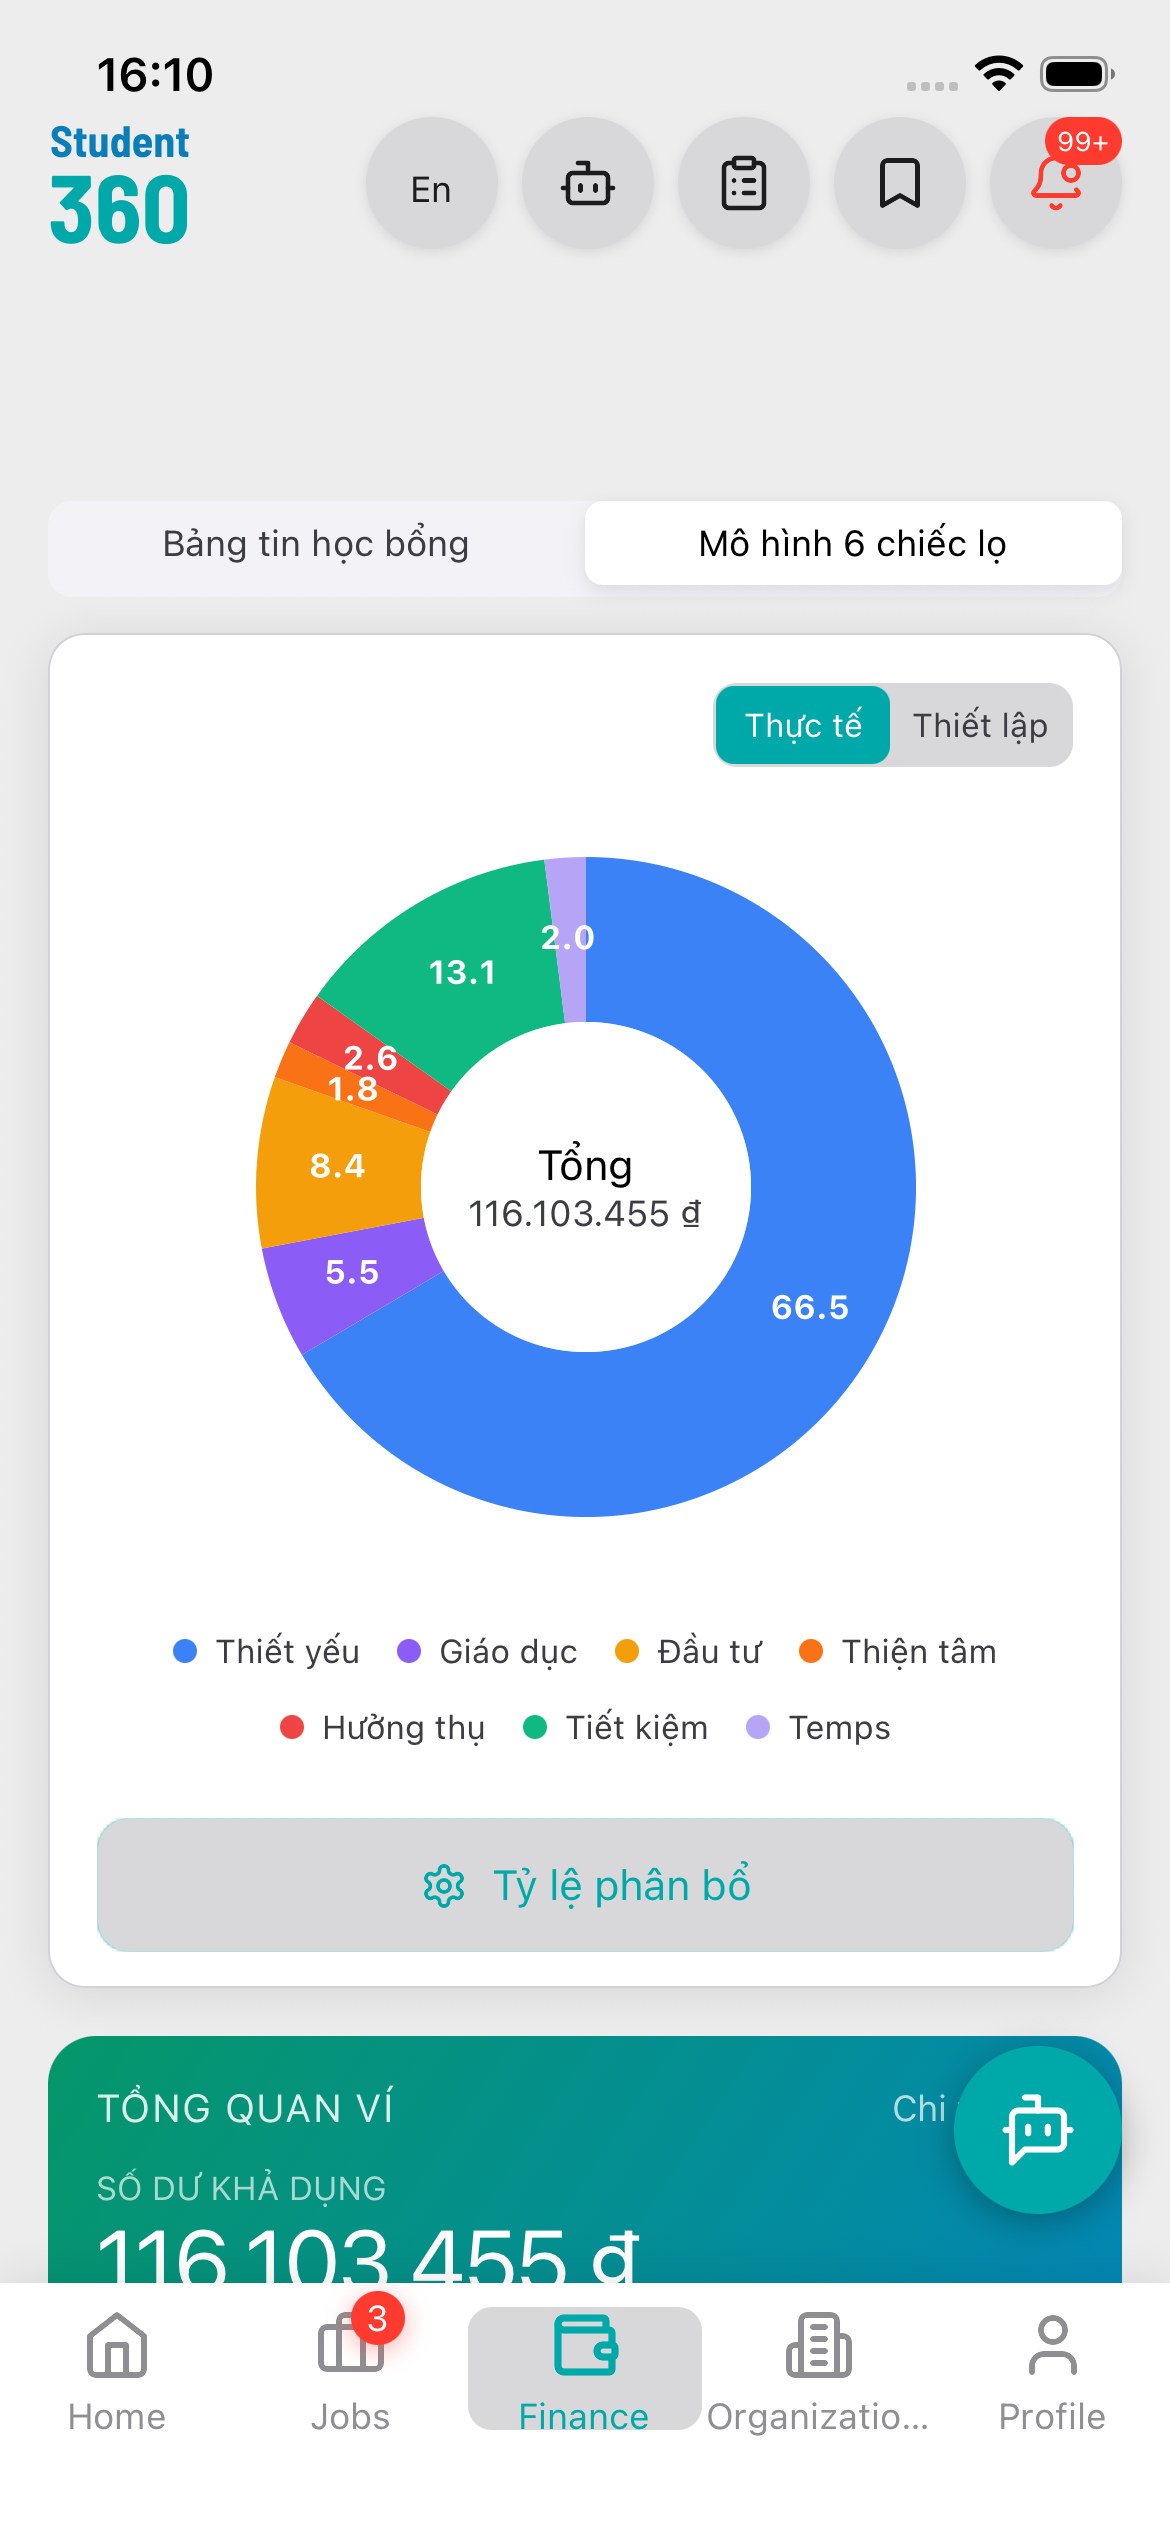
\includegraphics[width=\textwidth]{images/chapter4/mobile/wallet-overview.png}%
        }{%
            \rectbox{Hình ảnh ví 6 lọ tài chính trên Mobile}
        }
        \caption{Giao diện tổng quan ví 6 lọ trên thiết bị di động}
        \label{fig:mobile-6jars}
    \end{minipage}
    \hfill
    \begin{minipage}{0.44\textwidth}
        \centering
        \IfFileExists{images/chapter4/mobile/wallet-overview-detail.png}{%
            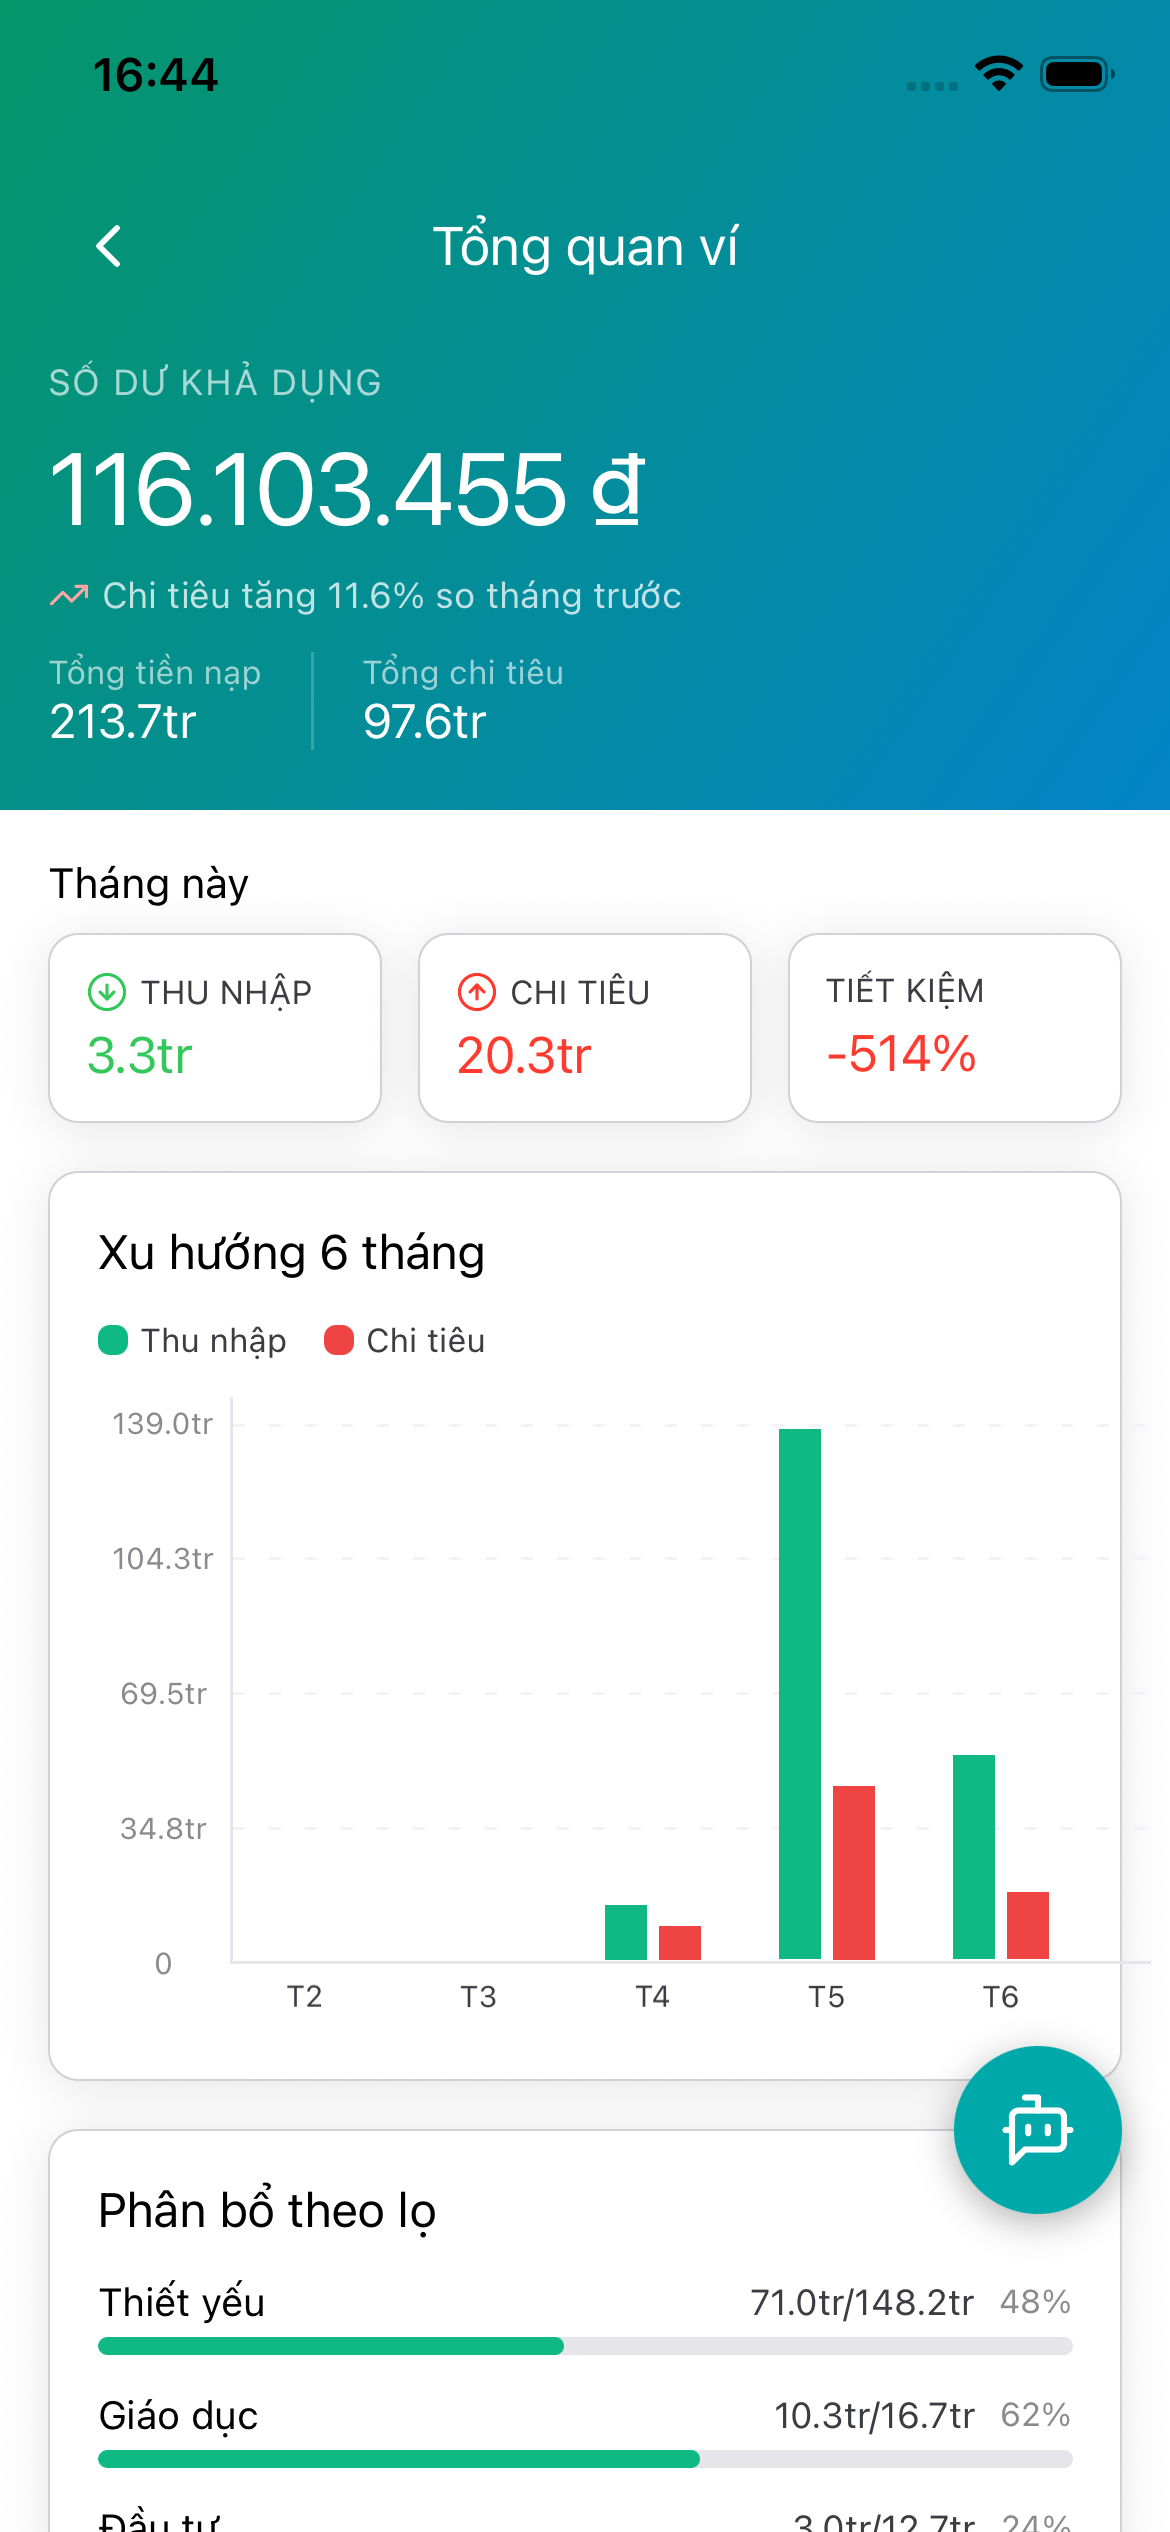
\includegraphics[width=\textwidth]{images/chapter4/mobile/wallet-overview-detail.png}%
        }{%
            \rectbox{Hình ảnh chi tiết xu hướng thu chi trên màn hình ví}
        }
        \caption{Xu hướng thu chi và phân bổ theo lọ trên màn hình tổng quan ví}
        \label{fig:mobile-wallet-detail}
    \end{minipage}
\end{figure}

\begin{figure}[H]
    \noindent\textbf{2.} \textbf{Chi tiết hũ:} Màn hình này hiển thị chi tiết số dư, lịch sử giao dịch và cấu hình riêng biệt của từng hũ tài chính. Sinh viên có thể chủ động cài đặt các mức cảnh báo chi tiêu vượt ngưỡng tại đây để kiểm soát dòng tiền tốt hơn.
    
    \vspace{0.2cm}
    \centering
    \IfFileExists{images/chapter4/mobile/jar-detail.png}{%
        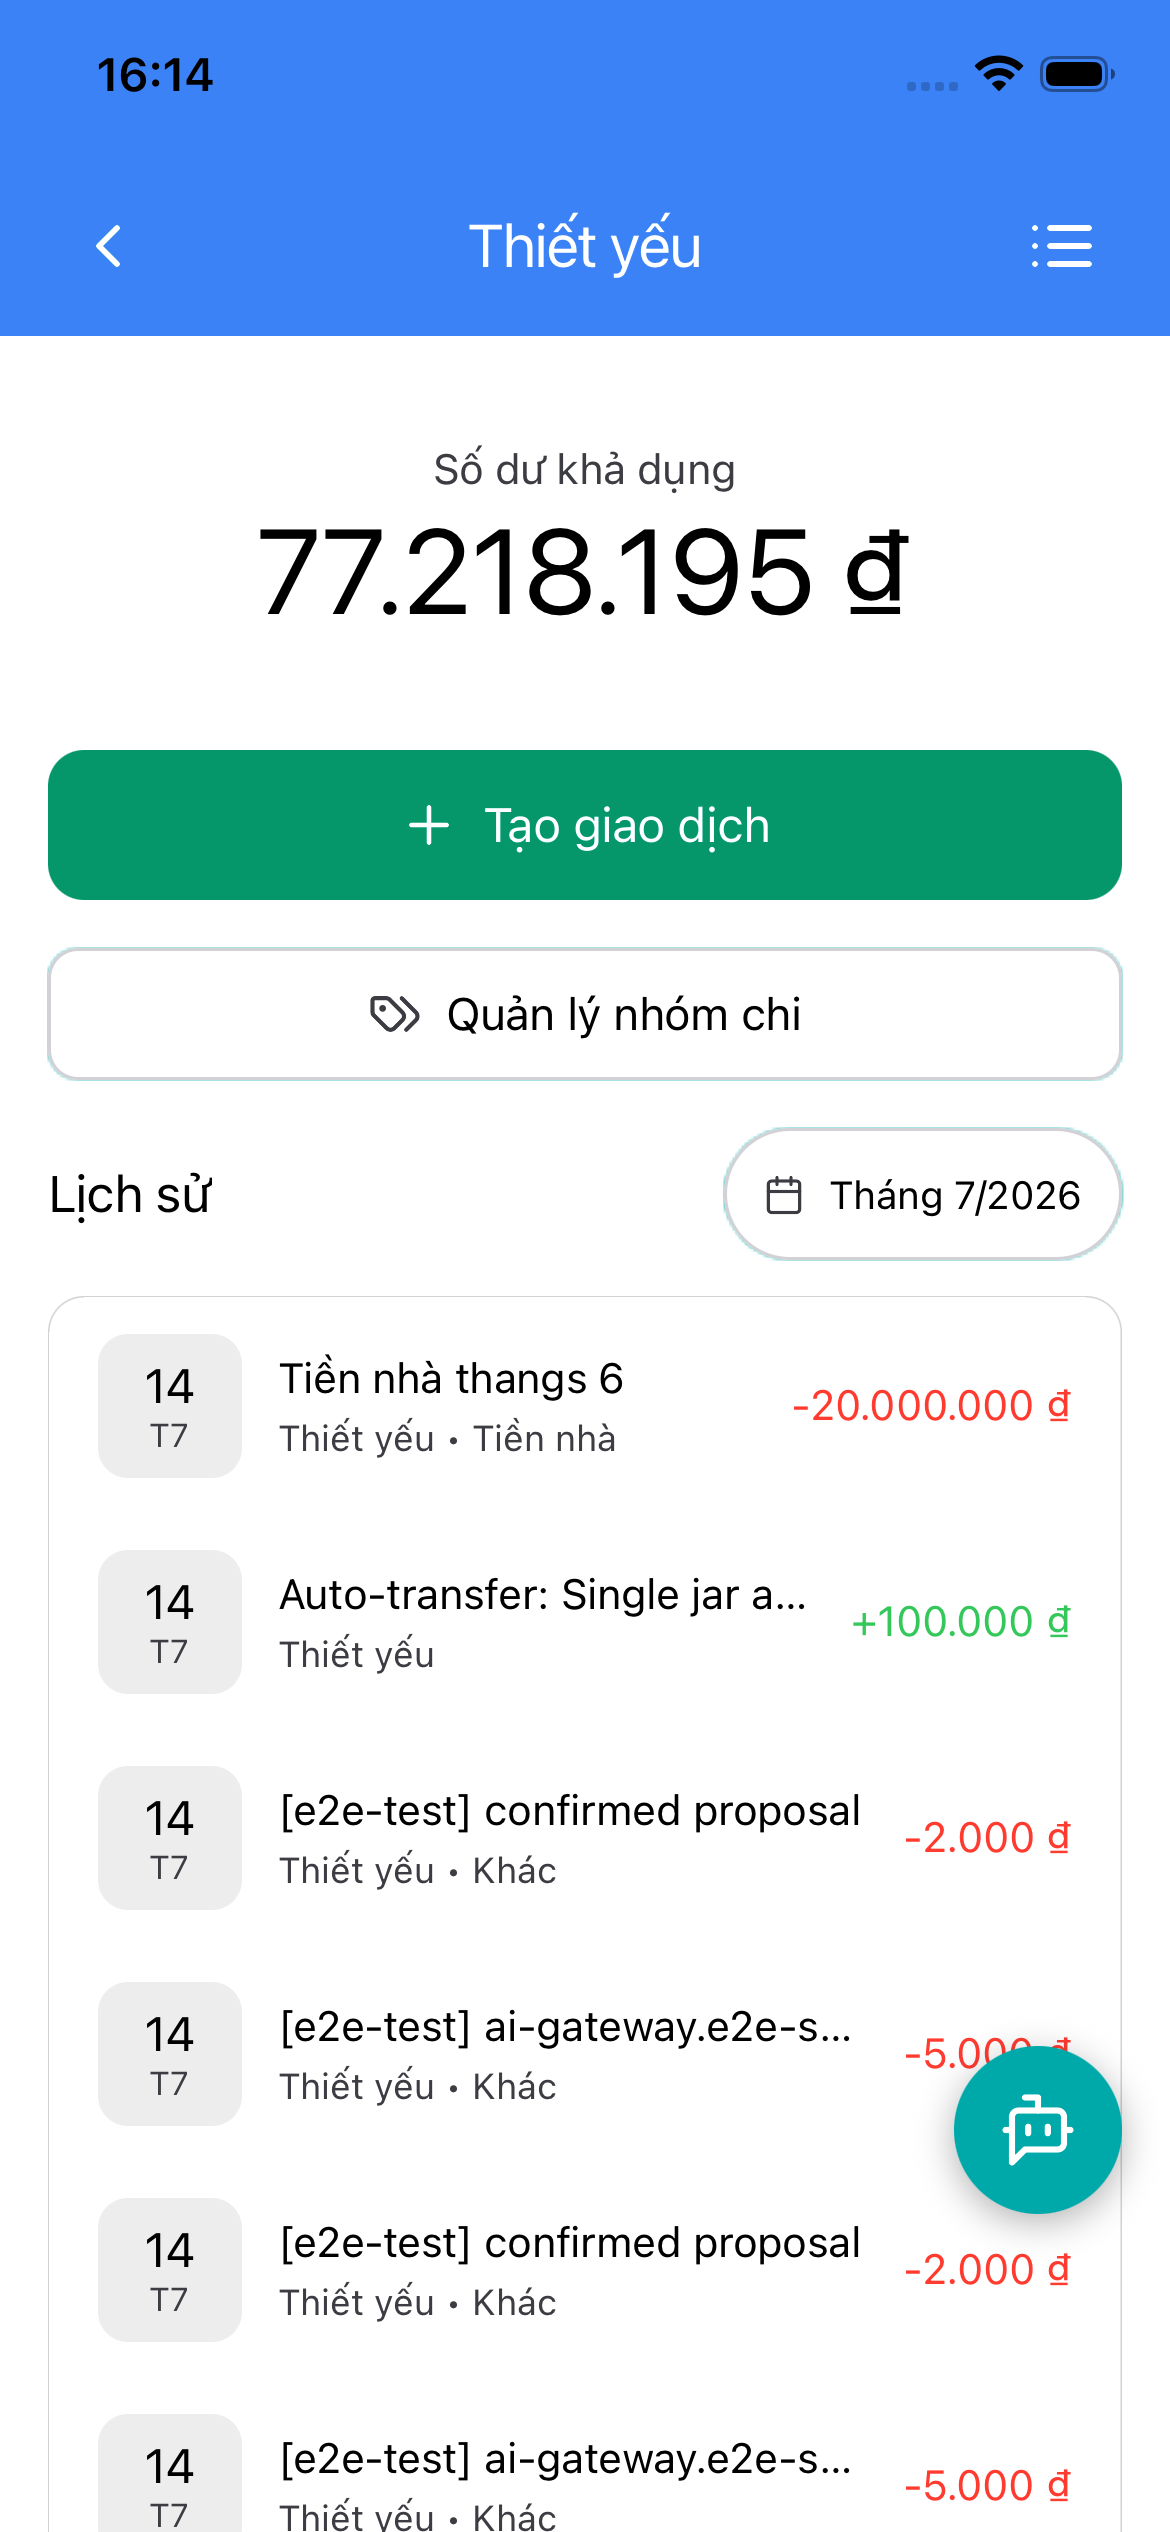
\includegraphics[width=0.4\textwidth]{images/chapter4/mobile/jar-detail.png}%
    }{%
        \rectbox{Hình ảnh màn hình chi tiết hũ trên Mobile}
    }
    \caption{Giao diện chi tiết hũ tài chính: số dư, ngưỡng cảnh báo và xu hướng dòng tiền}
    \label{fig:mobile-jar-detail}
\end{figure}

\begin{figure}[H]
    \noindent\textbf{3.} \textbf{Trò chuyện AI:} Màn hình này cho phép sinh viên trò chuyện trực tiếp với trợ lý tài chính ảo để truy vấn số dư hoặc thực hiện giao dịch nhanh bằng ngôn ngữ tự nhiên thông qua stream SSE thời gian thực. Giao diện cũng cung cấp một thanh menu sidebar để chuyển đổi nhanh các chủ đề. Sau khi AI Agent thực thi thành công một hành động tài chính (ví dụ: ghi nhận giao dịch mới qua lệnh tự nhiên), hệ thống áp dụng cơ chế Query Invalidation của React Query \cite{reactquery-docs} để tự động đánh dấu toàn bộ dữ liệu tài chính có liên quan là lỗi thời -- bao gồm số dư các hũ, lịch sử giao dịch và trang tổng quan -- rồi fetch lại ngầm và cập nhật UI tức thì mà không cần tải lại toàn bộ trang.
    
    \vspace{0.2cm}
    \centering
    \begin{minipage}{0.44\textwidth}
        \centering
        \IfFileExists{images/chapter4/mobile/ai-chat.png}{%
            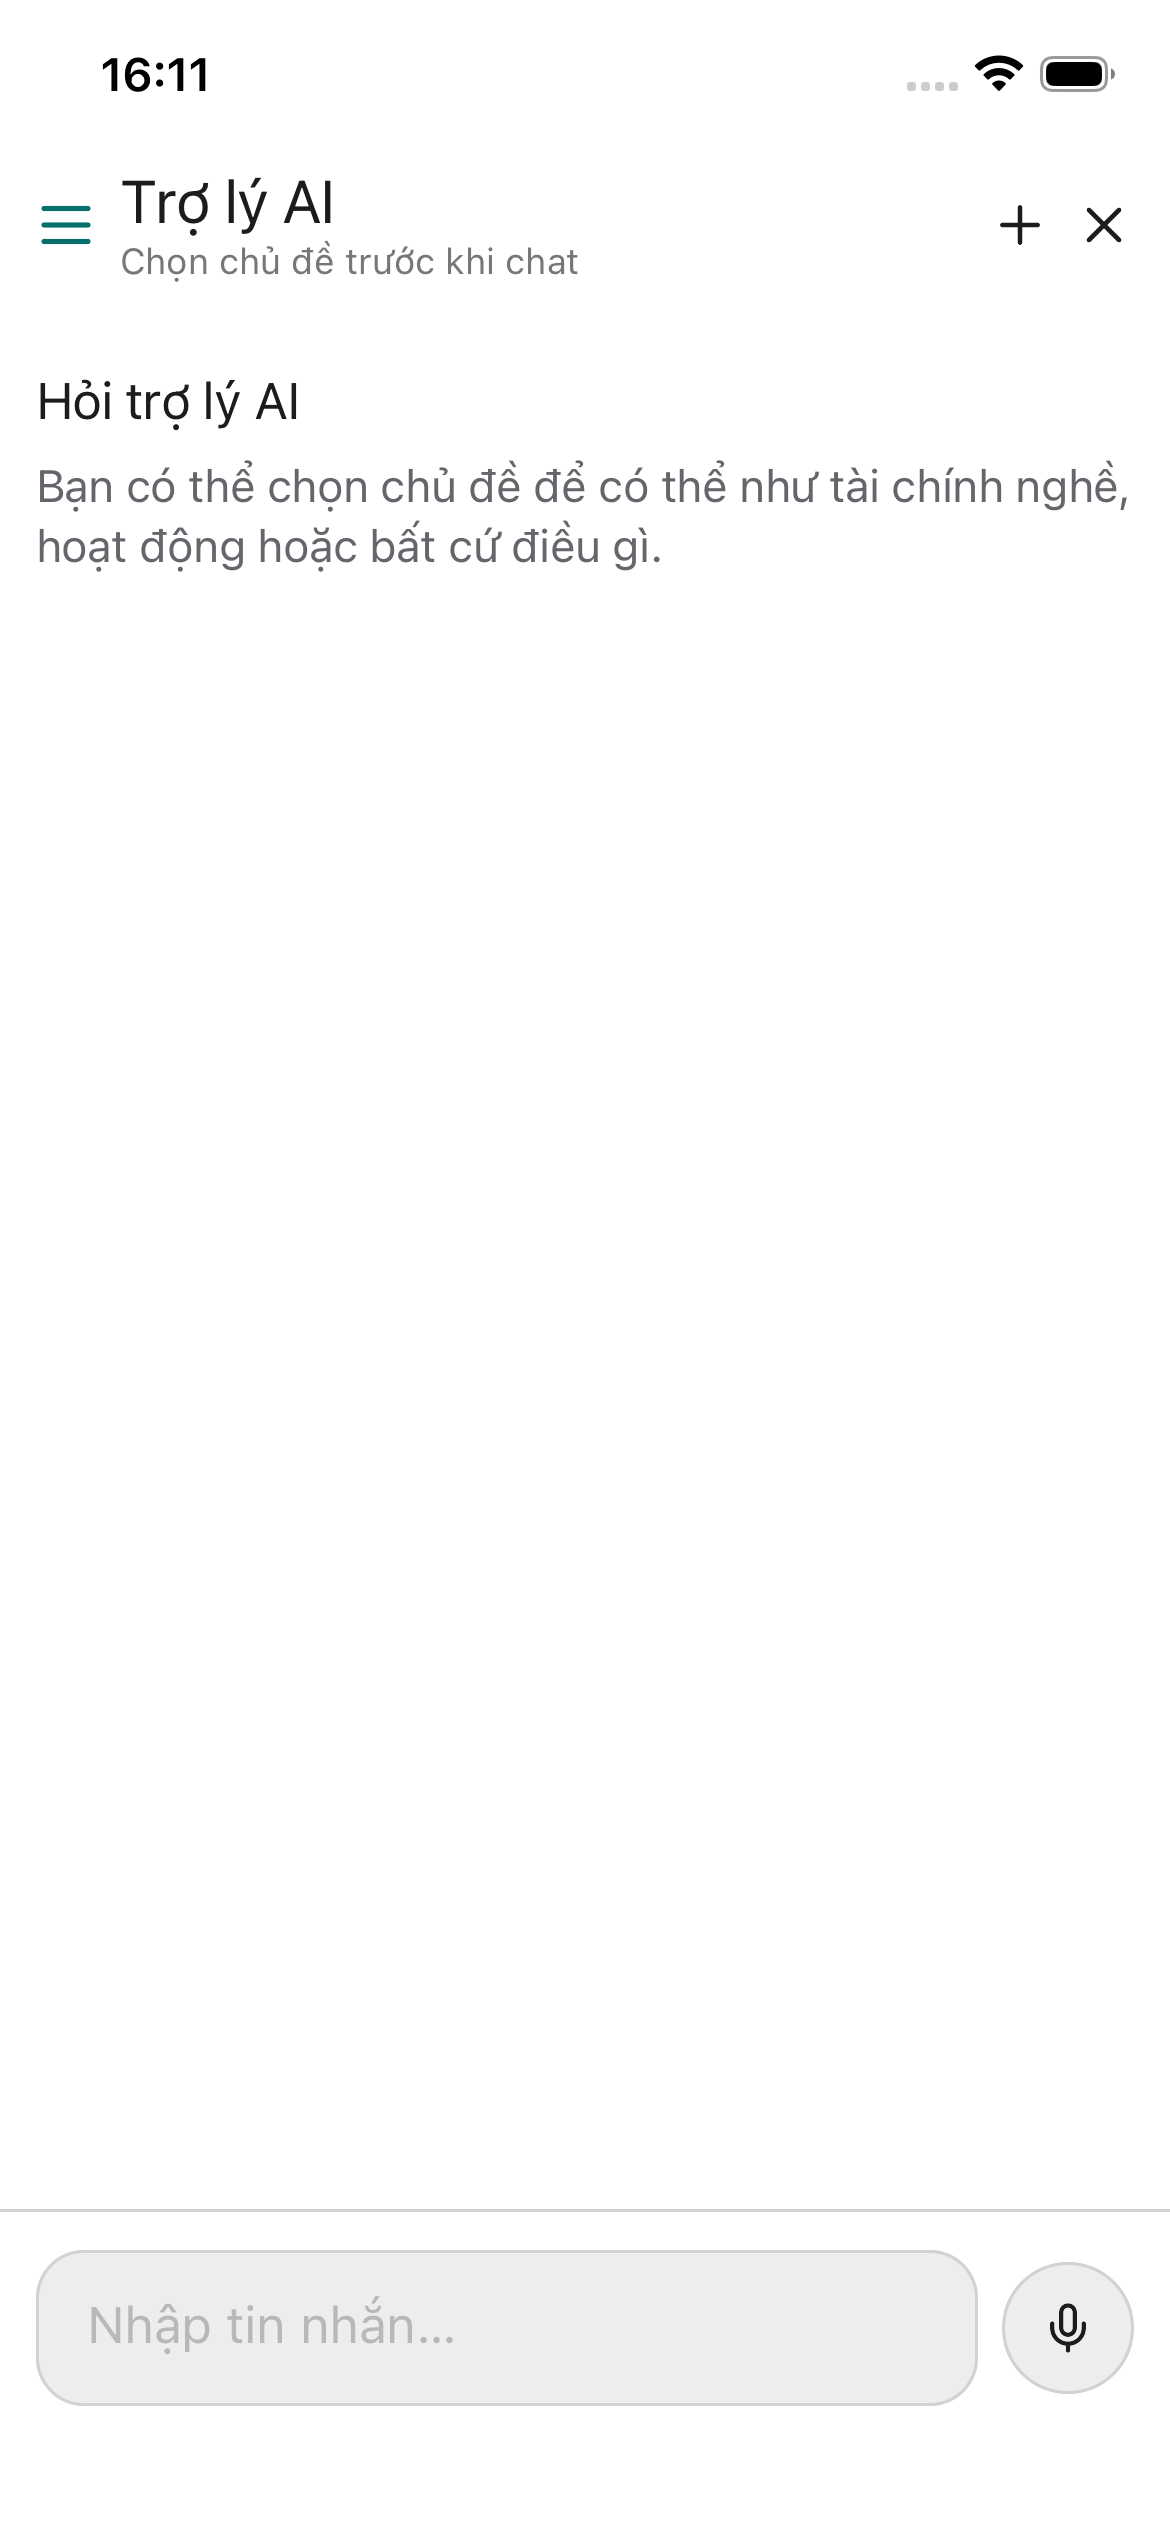
\includegraphics[width=\textwidth]{images/chapter4/mobile/ai-chat.png}%
        }{%
            \rectbox{Hình ảnh màn hình Chat AI Trợ lý}
        }
        \caption{Giao diện trò chuyện thời gian thực với trợ lý AI}
        \label{fig:mobile-aichat}
    \end{minipage}
    \hfill
    \begin{minipage}{0.44\textwidth}
        \centering
        \IfFileExists{images/chapter4/mobile/ai-chat-sidebar.png}{%
            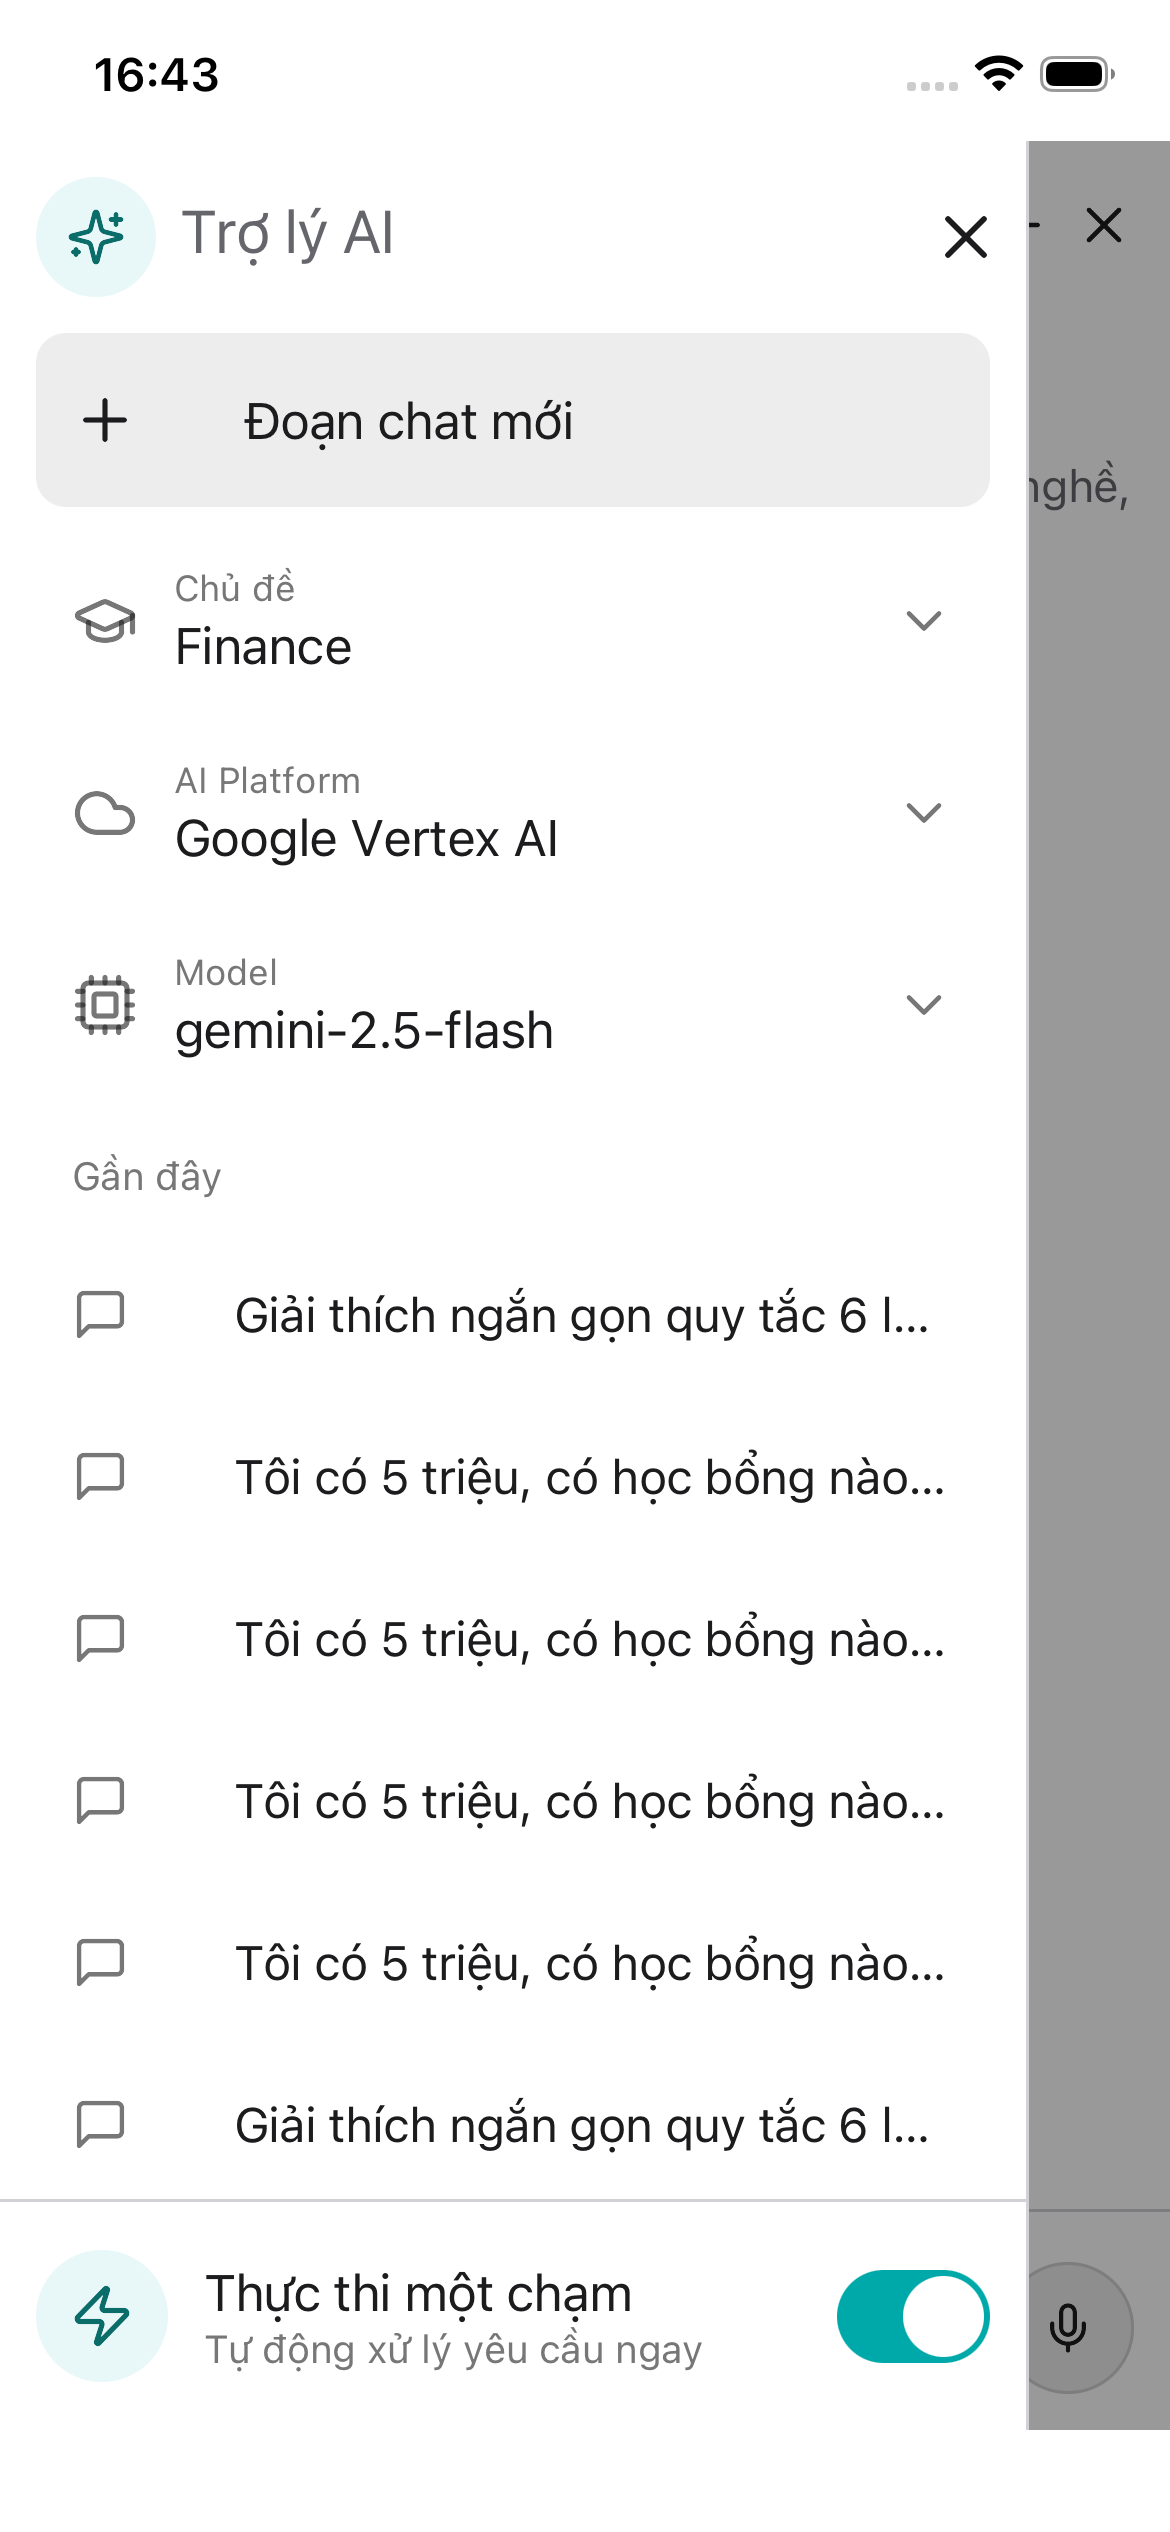
\includegraphics[width=\textwidth]{images/chapter4/mobile/ai-chat-sidebar.png}%
        }{%
            \rectbox{Hình ảnh bảng chọn chủ đề và mô hình AI}
        }
        \caption{Bảng chọn chủ đề, nền tảng AI và lịch sử trò chuyện gần đây}
        \label{fig:mobile-aichat-sidebar}
    \end{minipage}
\end{figure}

\begin{figure}[H]
    \noindent\textbf{4.} \textbf{Cấu hình phân bổ lọ:} Màn hình này hỗ trợ sinh viên kéo thả thanh trượt để thay đổi phần trăm phân bổ thu nhập tự động vào 6 hũ tài chính. Hệ thống ràng buộc tổng tỷ lệ luôn đạt chính xác 100\% trước khi lưu cấu hình mới.
    
    \vspace{0.2cm}
    \centering
    \IfFileExists{images/chapter4/mobile/jar-allocation.png}{%
        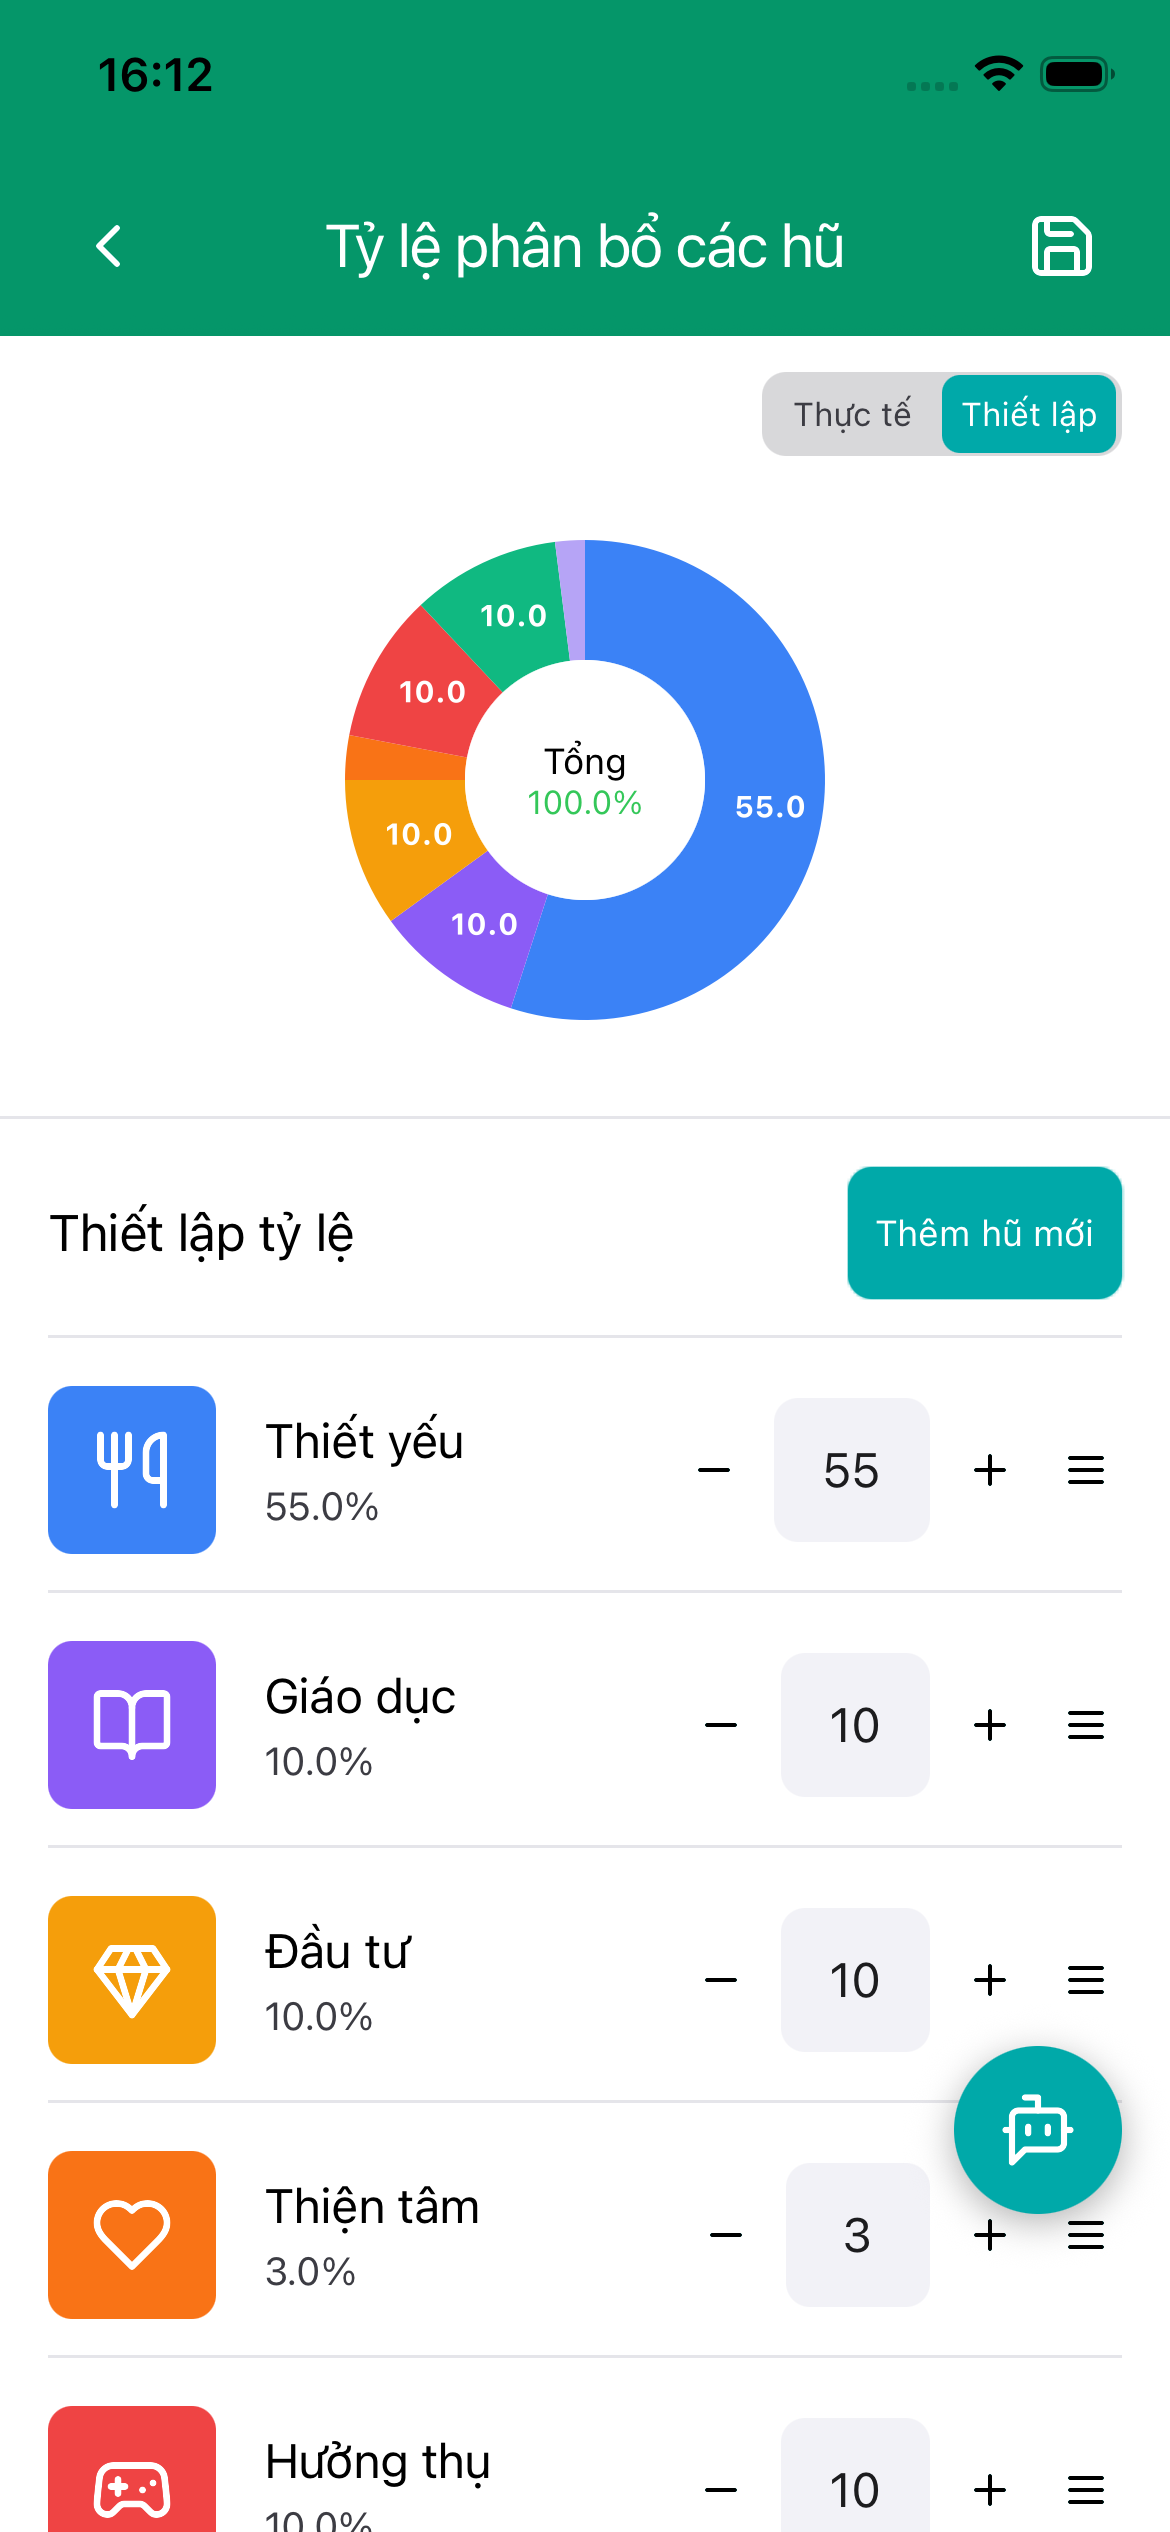
\includegraphics[width=0.4\textwidth]{images/chapter4/mobile/jar-allocation.png}%
    }{%
        \rectbox{Hình ảnh màn hình điều chỉnh tỷ lệ 6 lọ trên Mobile}
    }
    \caption{Giao diện cấu hình phần trăm phân bổ hũ tài chính (tổng luôn bằng 100\%)}
    \label{fig:mobile-jar-alloc}
\end{figure}
\clearpage

\begin{figure}[H]
    \noindent\textbf{5.} \textbf{Ghi chép giao dịch:} Màn hình này cung cấp biểu mẫu nhập giao dịch thu chi mới. Đối với các giao dịch thu nhập, hệ thống tự động hiển thị modal phân bổ nhanh vào các hũ theo tỷ lệ định cấu hình trước đó để chia tiền tự động. Ngay sau khi giao dịch được lưu thành công, mutation hook của React Query \cite{reactquery-docs} lập tức invalidate toàn bộ cache tài chính liên quan (số dư hũ, lịch sử, biểu đồ báo cáo), đảm bảo dữ liệu hiển thị luôn phản ánh chính xác trạng thái mới nhất mà không cần sinh viên phải tải lại ứng dụng.
    
    \vspace{0.2cm}
    \centering
    \begin{minipage}{0.44\textwidth}
        \centering
        \IfFileExists{images/chapter4/mobile/add-transaction.png}{%
            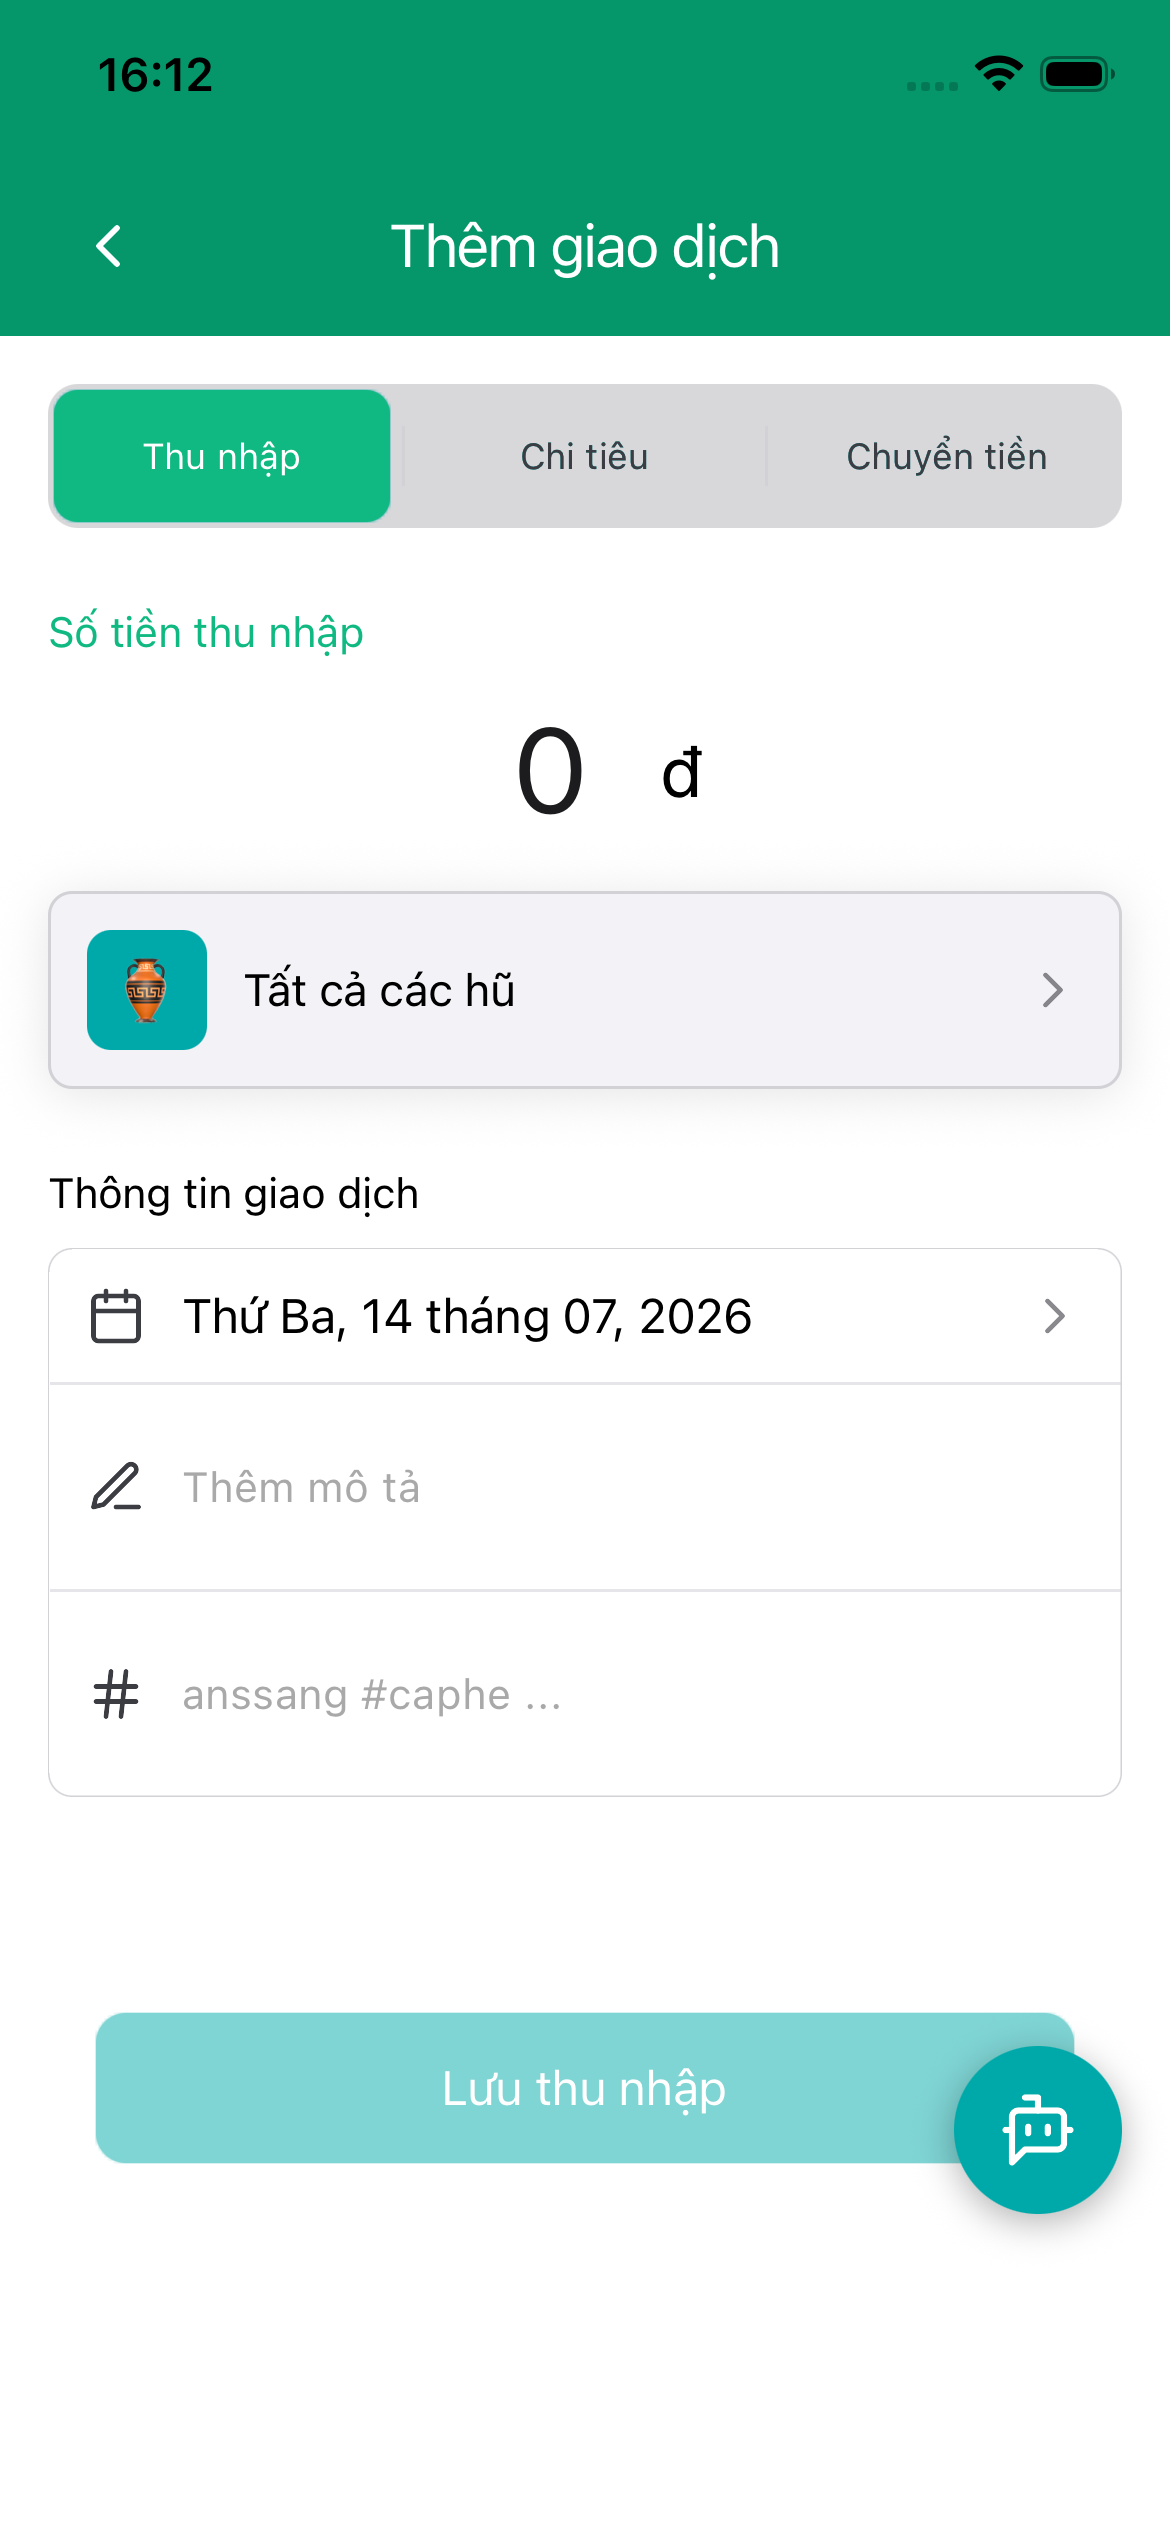
\includegraphics[width=\textwidth]{images/chapter4/mobile/add-transaction.png}%
        }{%
            \rectbox{Hình ảnh màn hình thêm mới giao dịch trên Mobile}
        }
        \caption{Giao diện biểu mẫu thêm mới giao dịch tài chính}
        \label{fig:mobile-add-transaction}
    \end{minipage}
    \hfill
    \begin{minipage}{0.44\textwidth}
        \centering
        \IfFileExists{images/chapter4/mobile/add-transaction-allocation.png}{%
            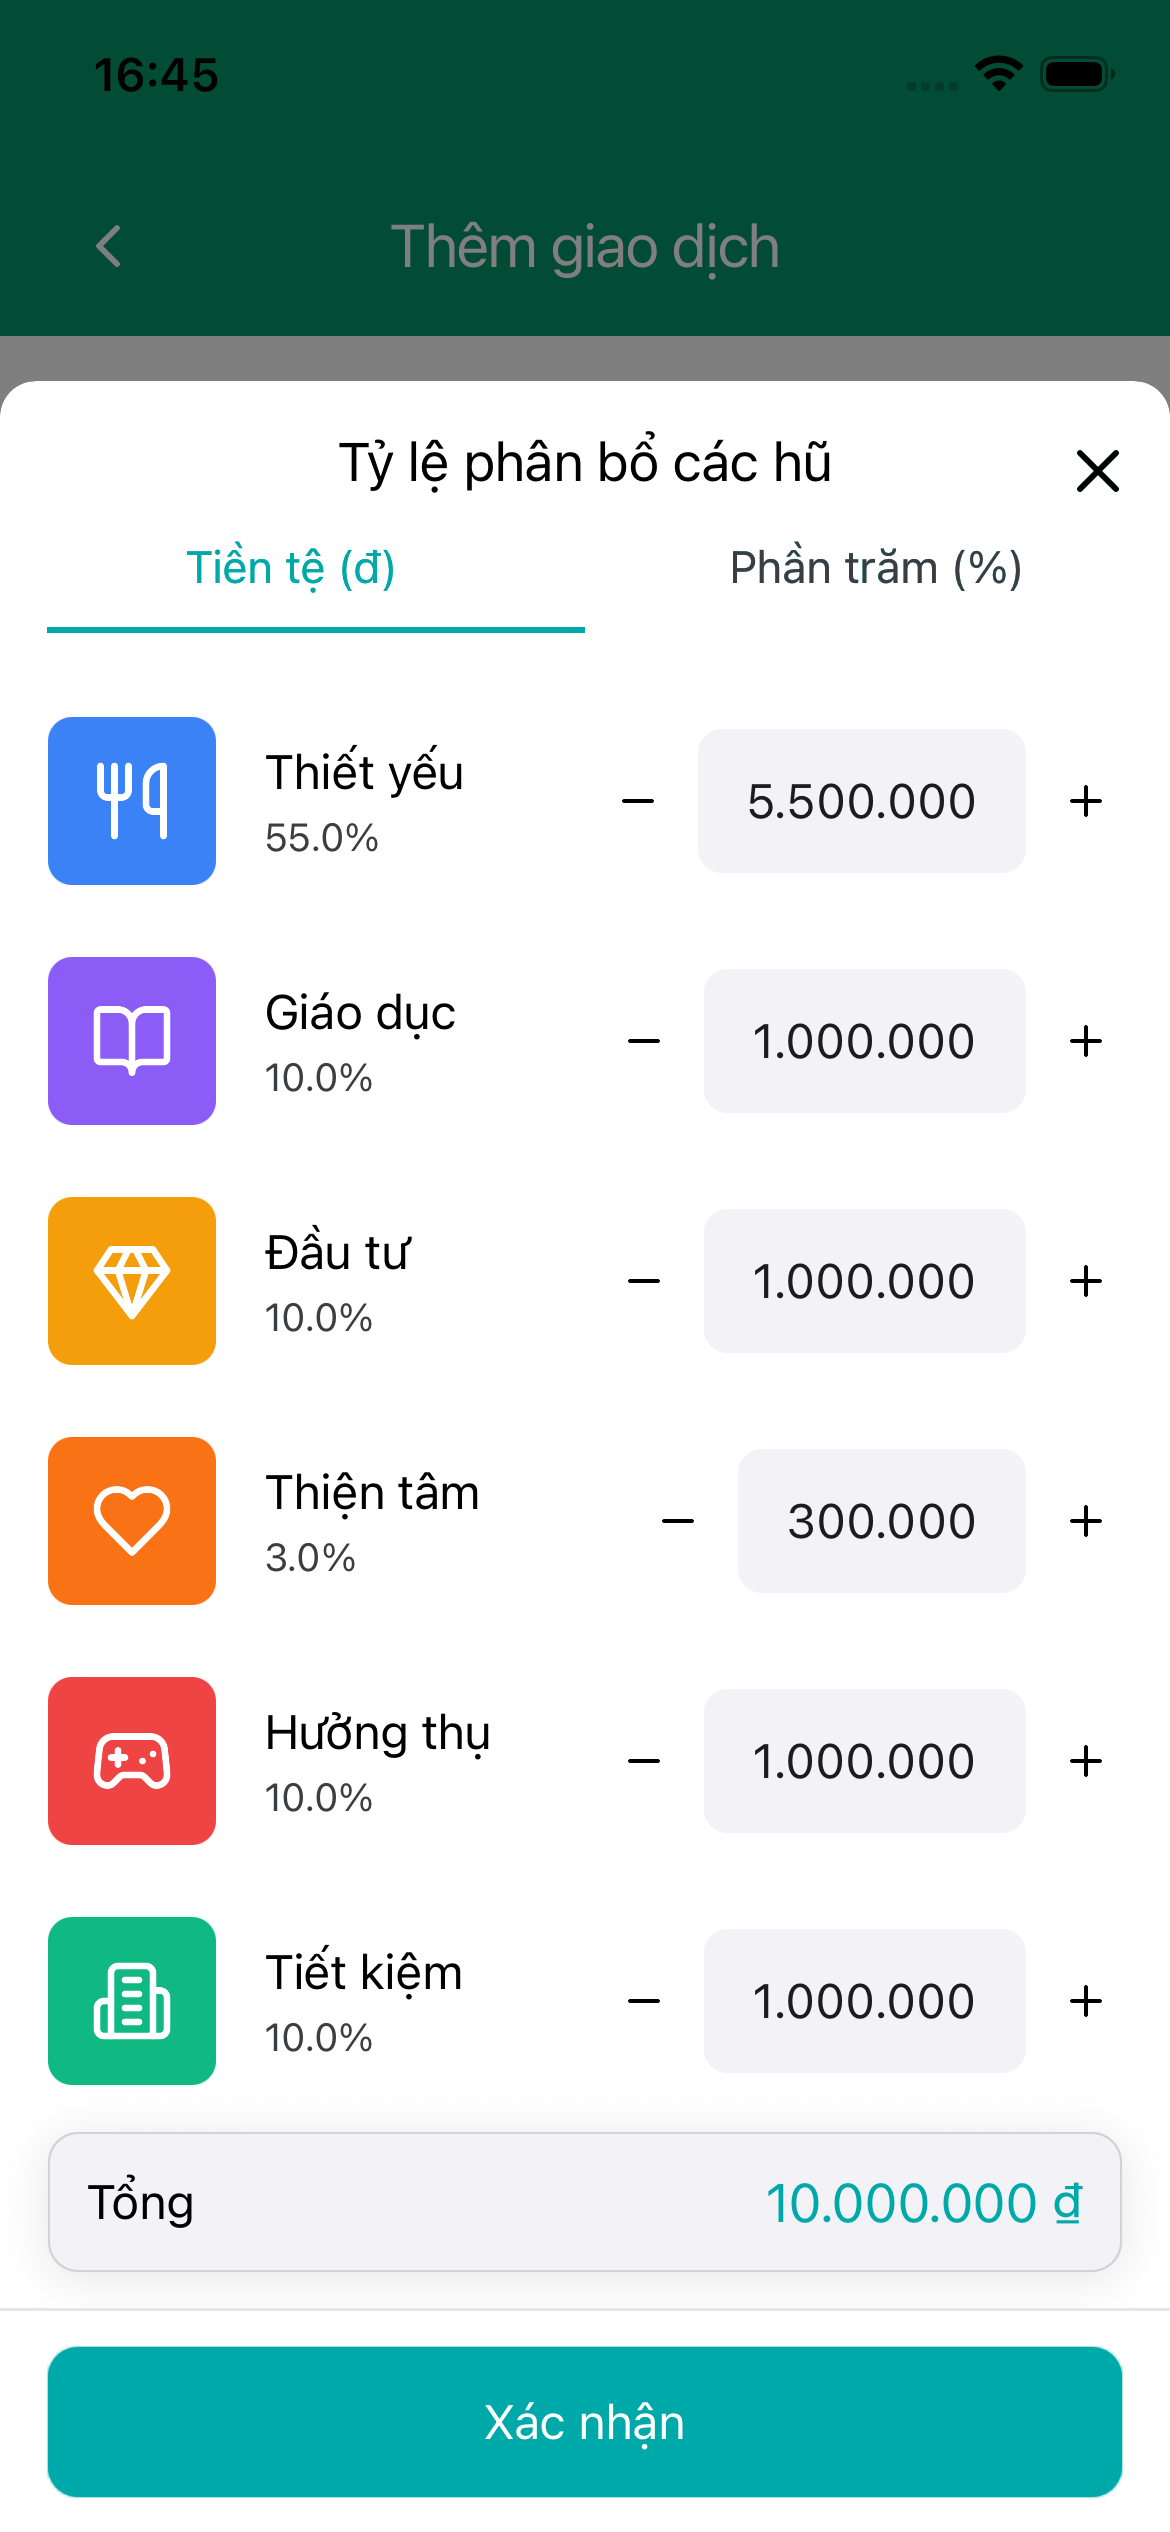
\includegraphics[width=\textwidth]{images/chapter4/mobile/add-transaction-allocation.png}%
        }{%
            \rectbox{Hình ảnh modal thiết lập tỷ lệ phân bổ khi thêm thu nhập}
        }
        \caption{Modal thiết lập tỷ lệ phân bổ vào các hũ khi ghi nhận thu nhập}
        \label{fig:mobile-add-transaction-allocation}
    \end{minipage}
\end{figure}

\begin{figure}[H]
    \noindent\textbf{6.} \textbf{Lịch sử giao dịch:} Màn hình này liệt kê chi tiết các giao dịch thu chi đã được ghi nhận trong hệ thống. Sinh viên có thể tra cứu nhanh theo nội dung giao dịch hoặc lọc giao dịch theo hũ cụ thể và mốc thời gian.
    
    \vspace{0.2cm}
    \centering
    \IfFileExists{images/chapter4/mobile/transaction-history.png}{%
        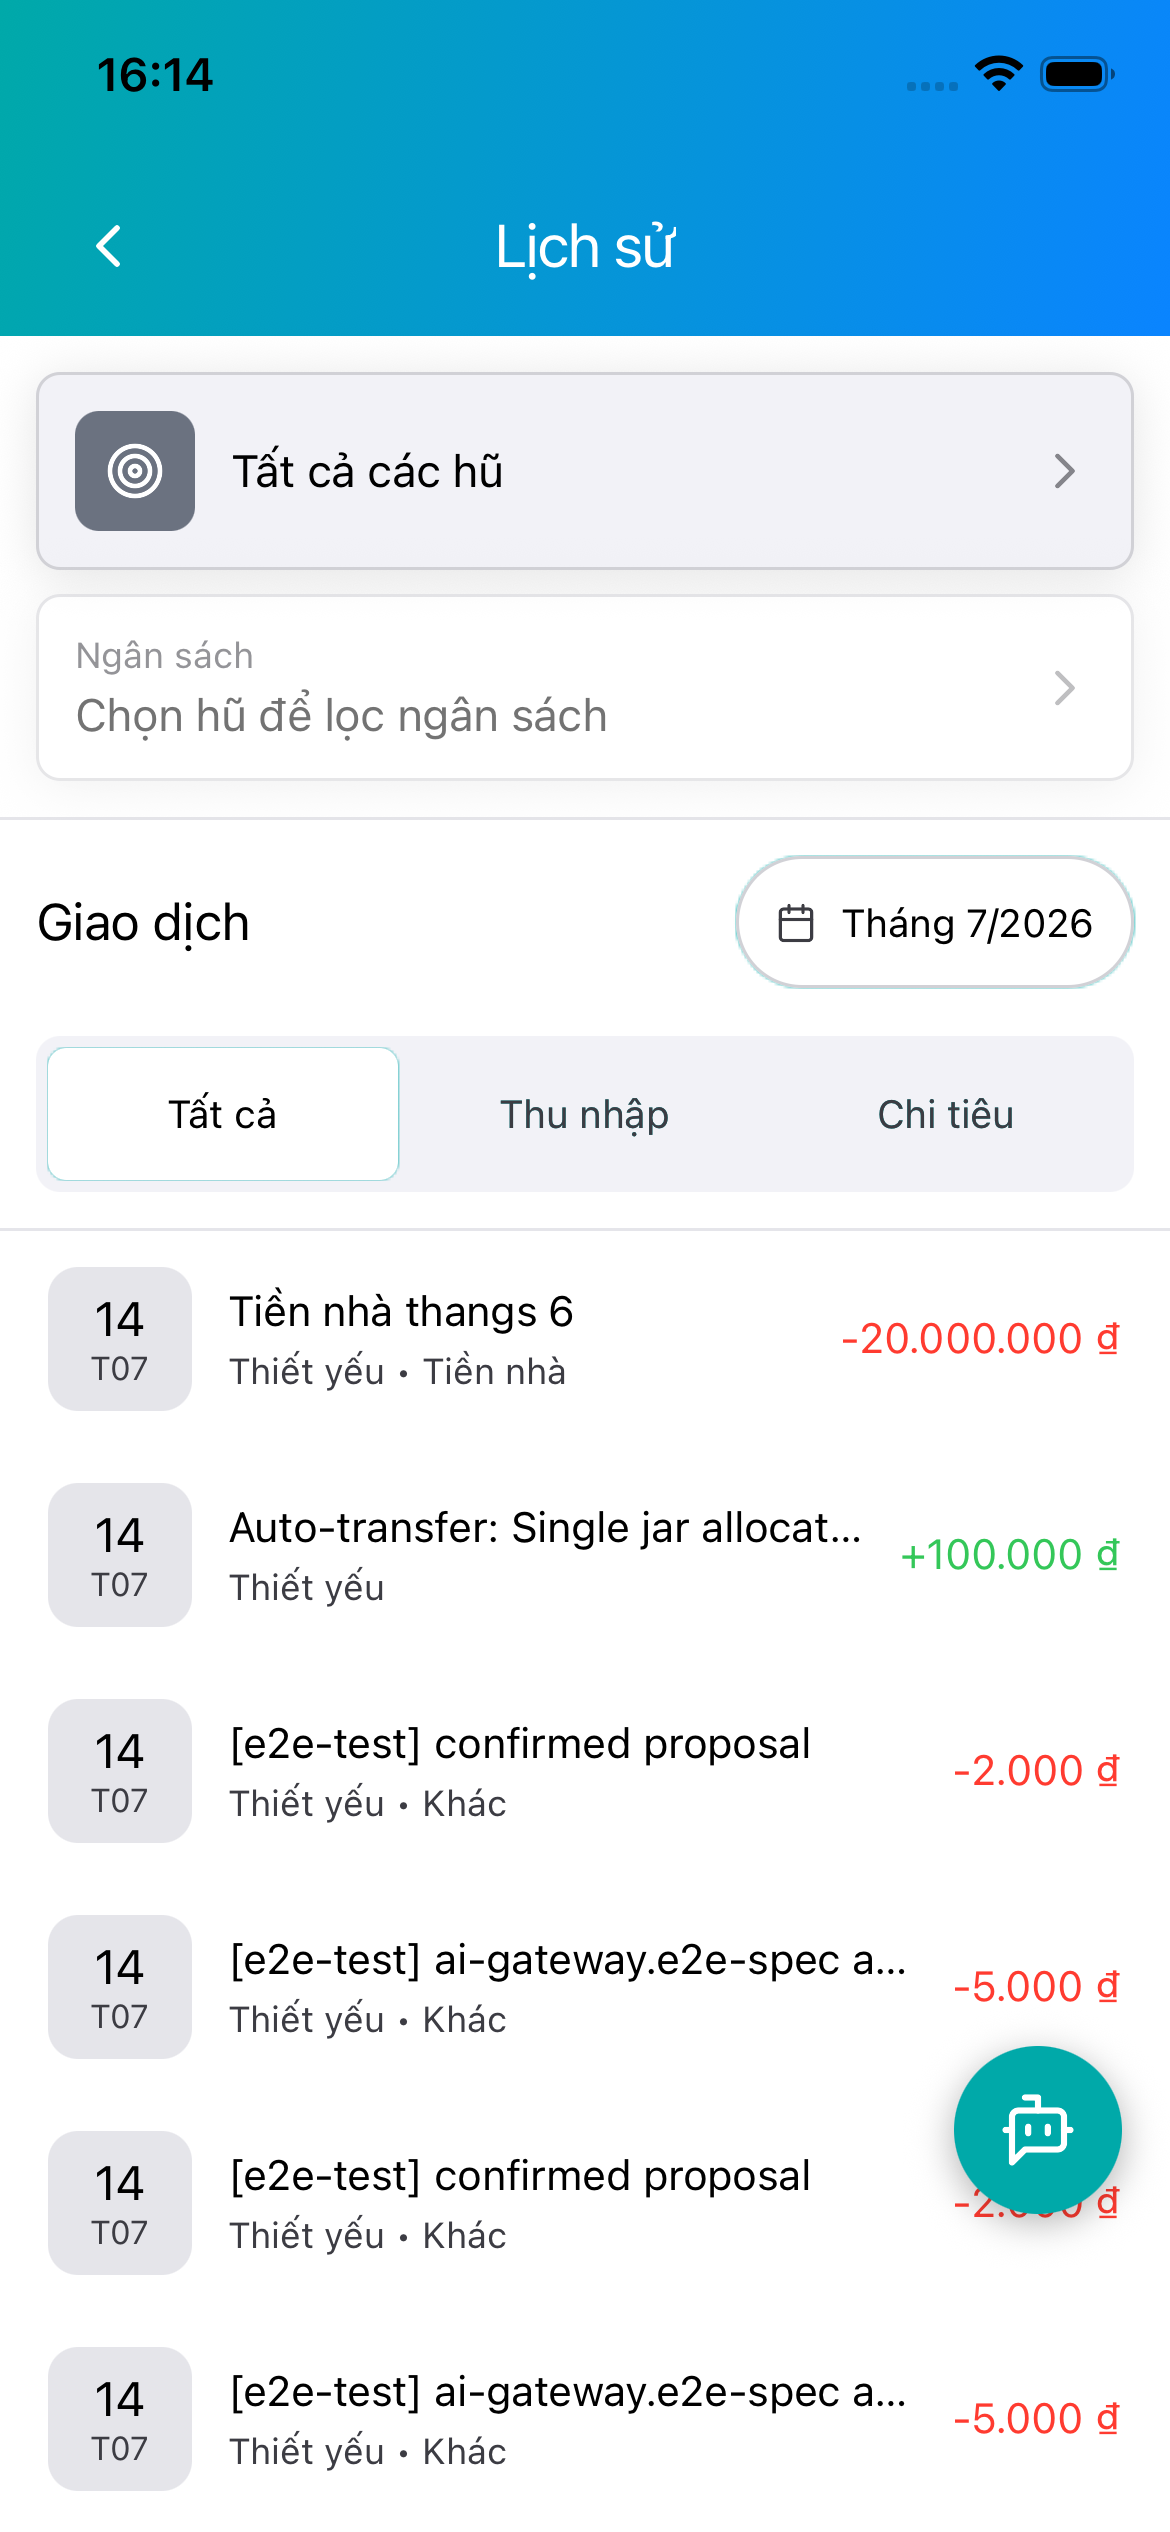
\includegraphics[width=0.4\textwidth]{images/chapter4/mobile/transaction-history.png}%
    }{%
        \rectbox{Hình ảnh danh sách lịch sử giao dịch trên Mobile}
    }
    \caption{Giao diện danh sách lịch sử giao dịch, hỗ trợ tìm kiếm và lọc theo hũ/thời gian}
    \label{fig:mobile-transaction-history}
\end{figure}
\clearpage

\begin{figure}[H]
    \noindent\textbf{7.} \textbf{Lịch chuyển tiền tự động:} Màn hình này cho phép thiết lập và quản lý các giao dịch chuyển tiền tự động định kỳ giữa các hũ tài chính. Người dùng có thể chỉnh sửa số tiền, chu kỳ lặp lại và trạng thái kích hoạt của lịch chuyển.
    
    \vspace{0.2cm}
    \centering
    \begin{minipage}{0.44\textwidth}
        \centering
        \IfFileExists{images/chapter4/mobile/auto-transfer.png}{%
            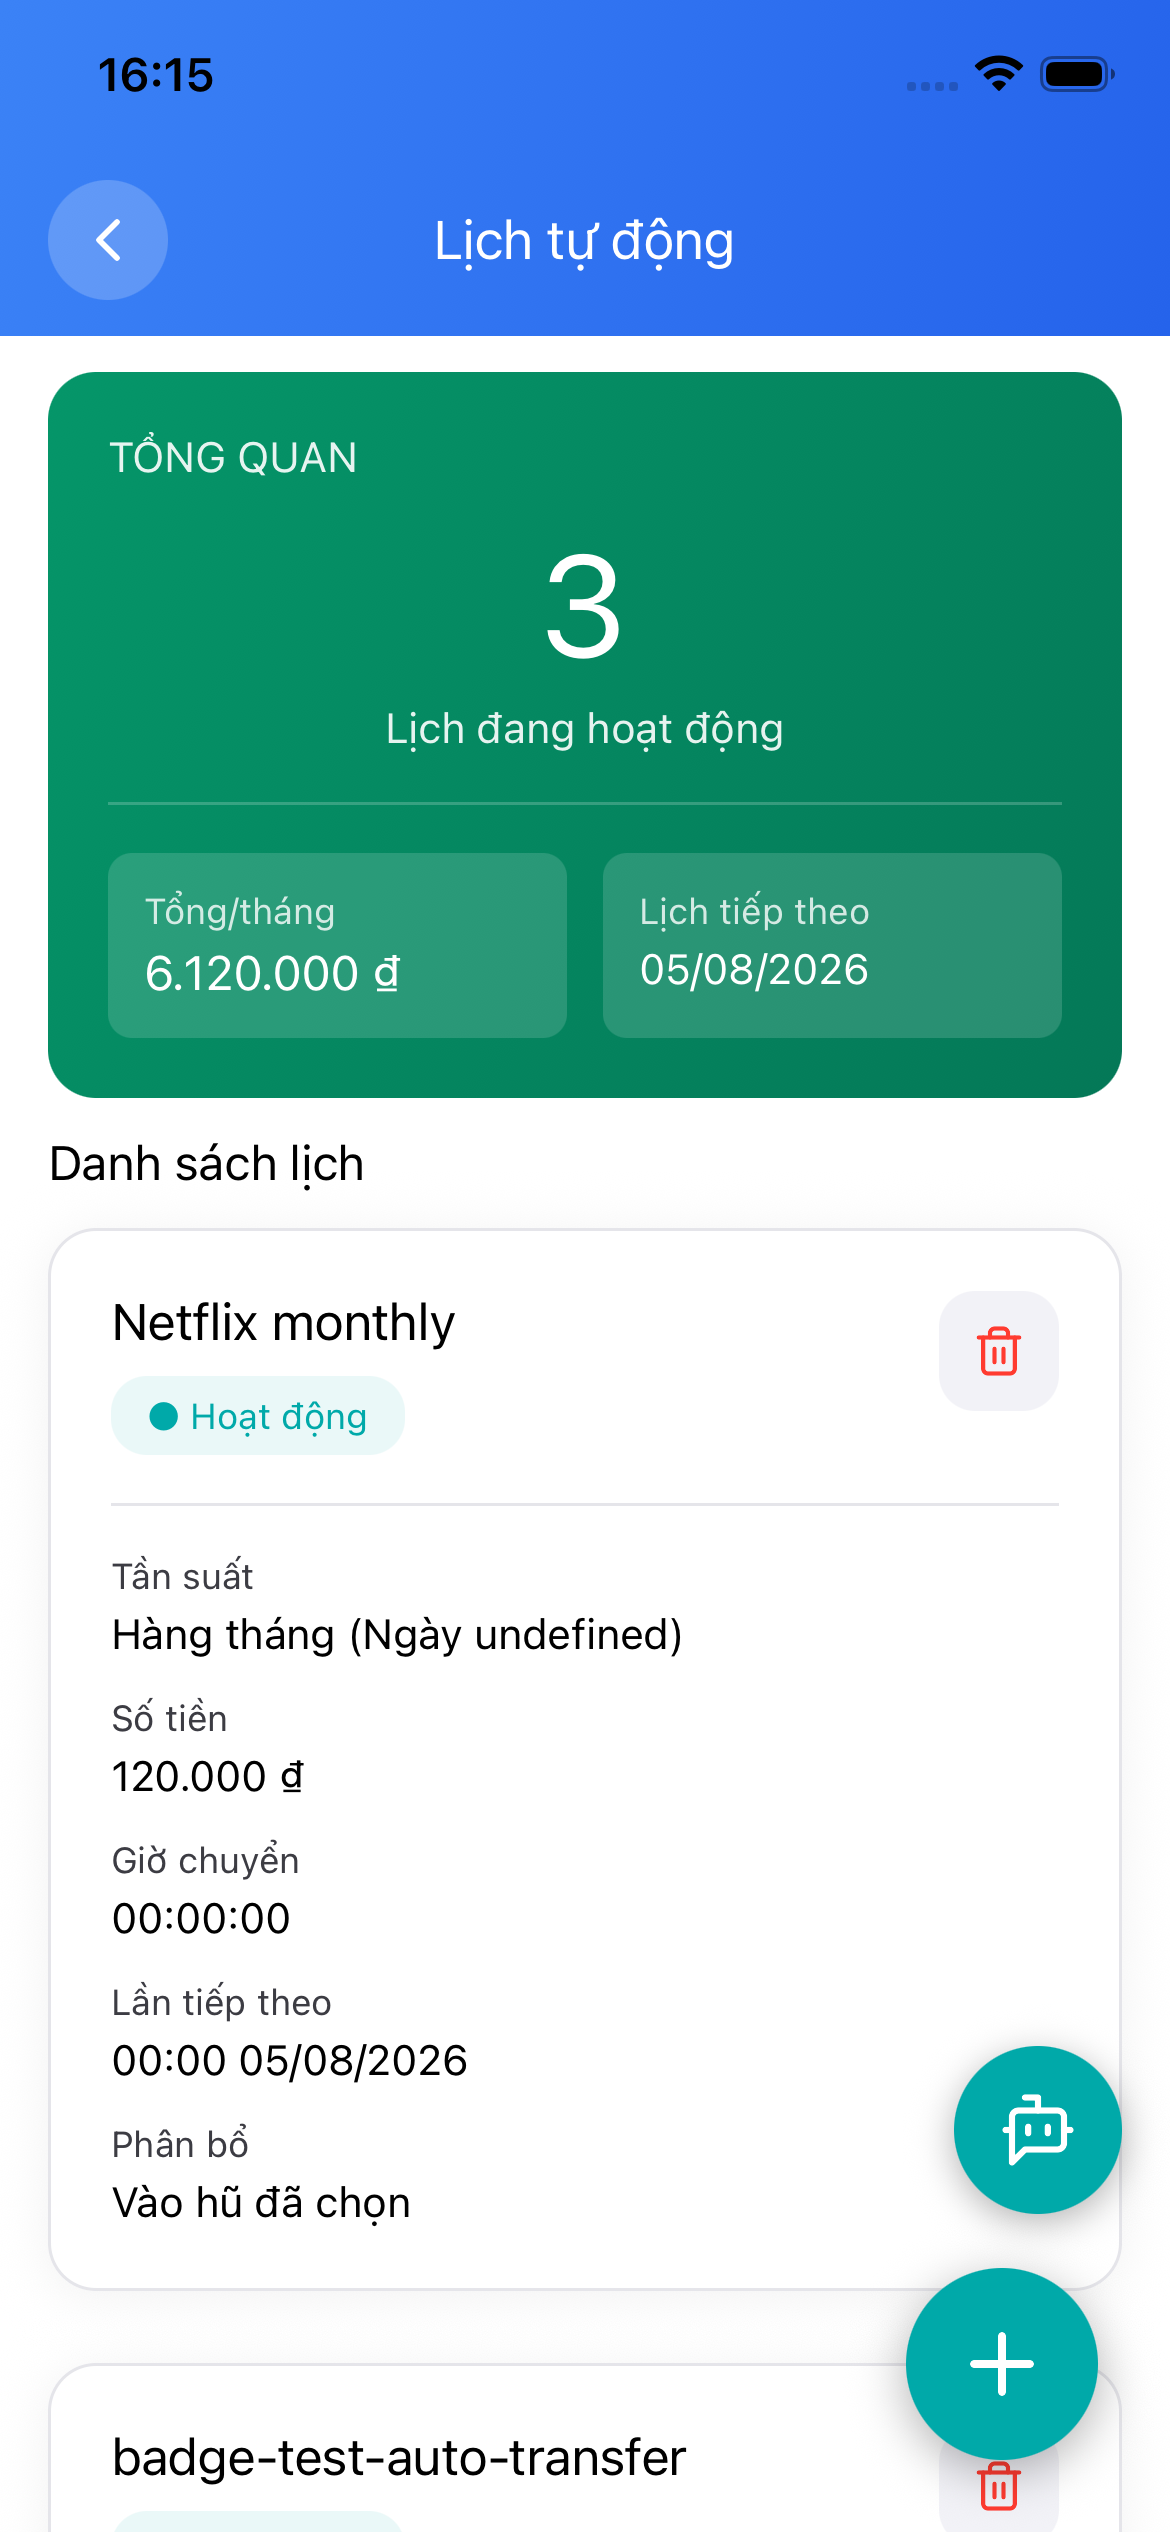
\includegraphics[width=\textwidth]{images/chapter4/mobile/auto-transfer.png}%
        }{%
            \rectbox{Hình ảnh màn hình quản lý lịch chuyển tự động trên Mobile}
        }
        \caption{Giao diện quản lý lịch chuyển tiền tự động}
        \label{fig:mobile-auto-transfer}
    \end{minipage}
    \hfill
    \begin{minipage}{0.44\textwidth}
        \centering
        \IfFileExists{images/chapter4/mobile/auto-transfer-edit.png}{%
            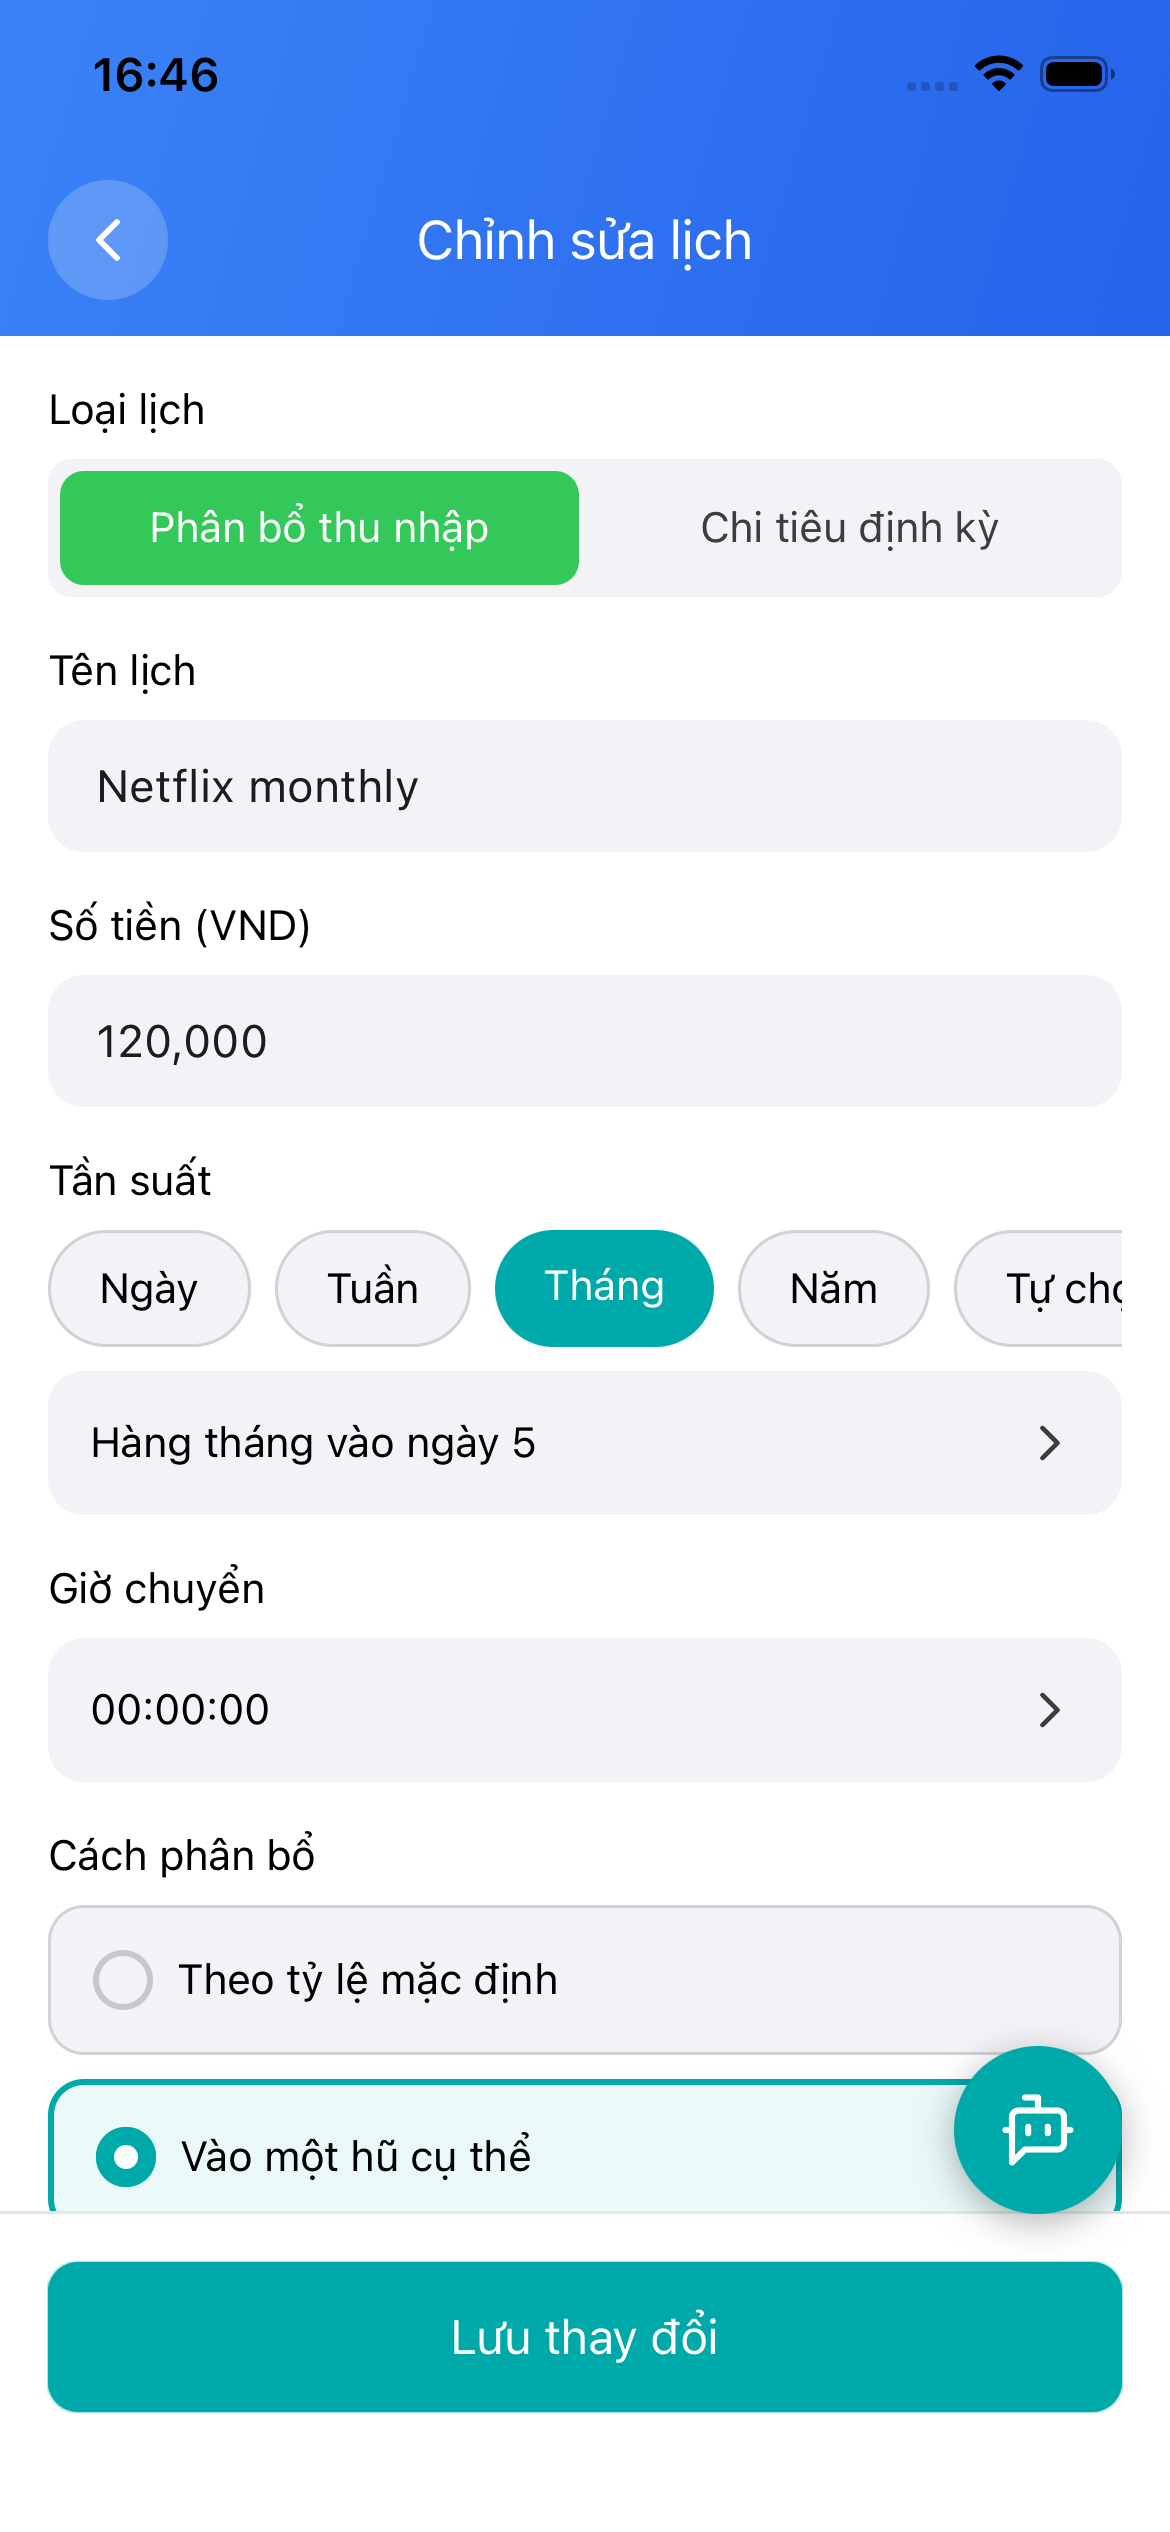
\includegraphics[width=\textwidth]{images/chapter4/mobile/auto-transfer-edit.png}%
        }{%
            \rectbox{Hình ảnh biểu mẫu chỉnh sửa lịch chuyển tiền tự động}
        }
        \caption{Biểu mẫu chỉnh sửa lịch chuyển tiền tự động}
        \label{fig:mobile-auto-transfer-edit}
    \end{minipage}
\end{figure}

\begin{figure}[H]
    \noindent\textbf{8.} \textbf{Báo cáo tài chính:} Màn hình này hiển thị biểu đồ thống kê các khoản thu chi định kỳ và phân bổ dòng tiền. Tại đây tích hợp mô-đun AI Insights tự động nhận định thói quen tiêu dùng của sinh viên và gửi các khuyến nghị tối ưu tài chính.
    
    \vspace{0.2cm}
    \centering
    \begin{minipage}{0.44\textwidth}
        \centering
        \IfFileExists{images/chapter4/mobile/financial-report.png}{%
            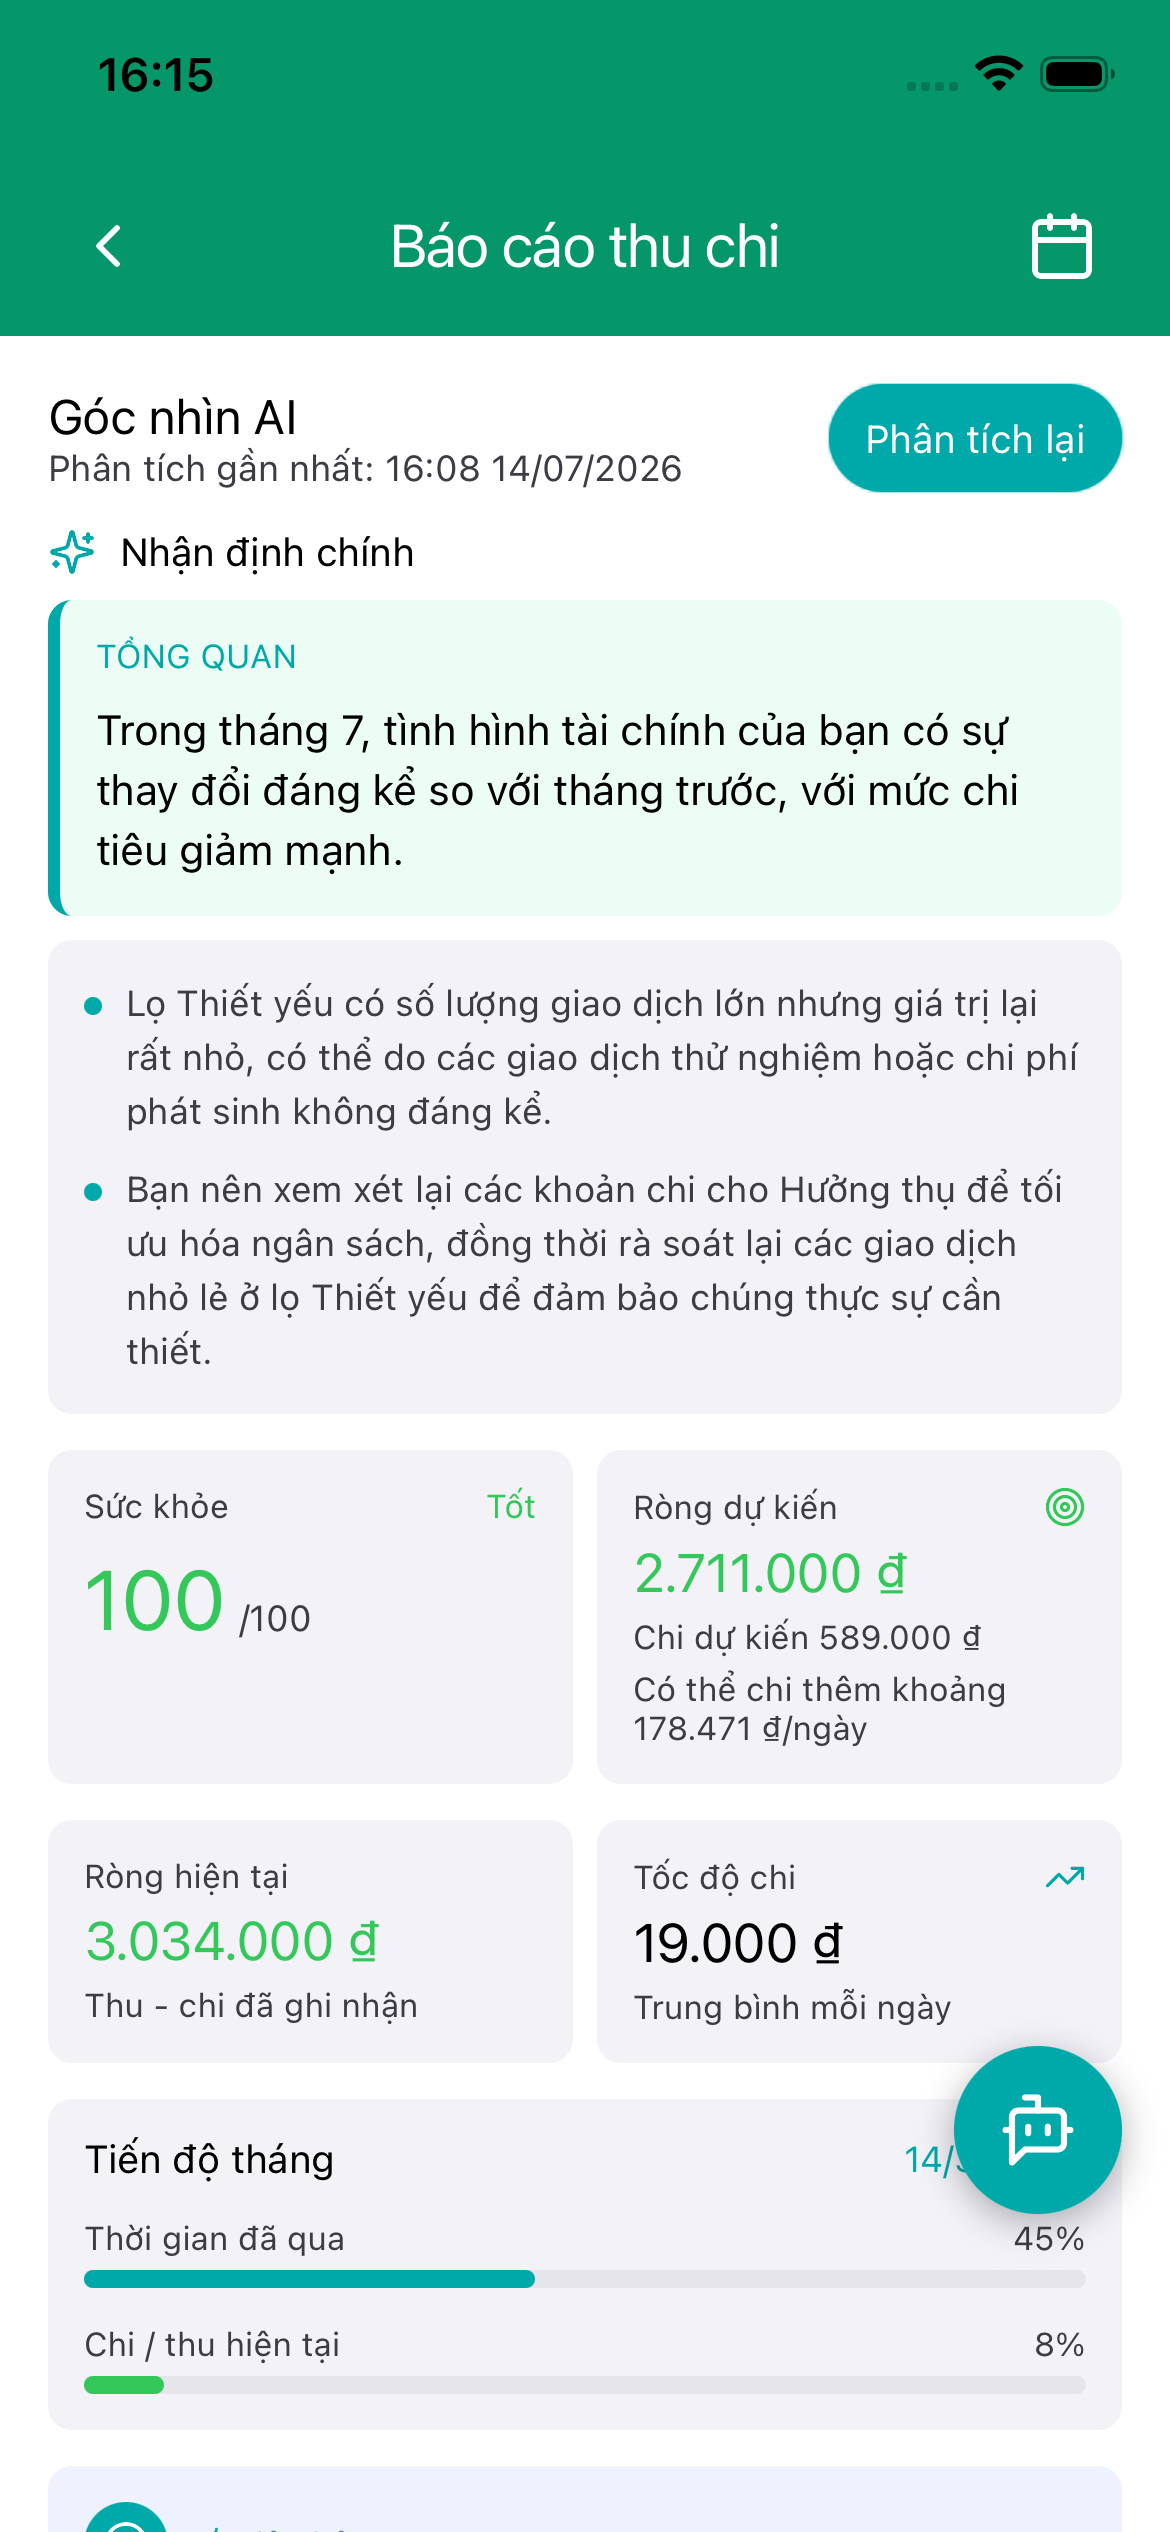
\includegraphics[width=\textwidth]{images/chapter4/mobile/financial-report.png}%
        }{%
            \rectbox{Hình ảnh màn hình báo cáo phân tích tài chính trên Mobile}
        }
        \caption{Giao diện báo cáo phân tích tài chính chi tiêu}
        \label{fig:mobile-financial-report}
    \end{minipage}
    \hfill
    \begin{minipage}{0.44\textwidth}
        \centering
        \IfFileExists{images/chapter4/mobile/financial-report-chart.png}{%
            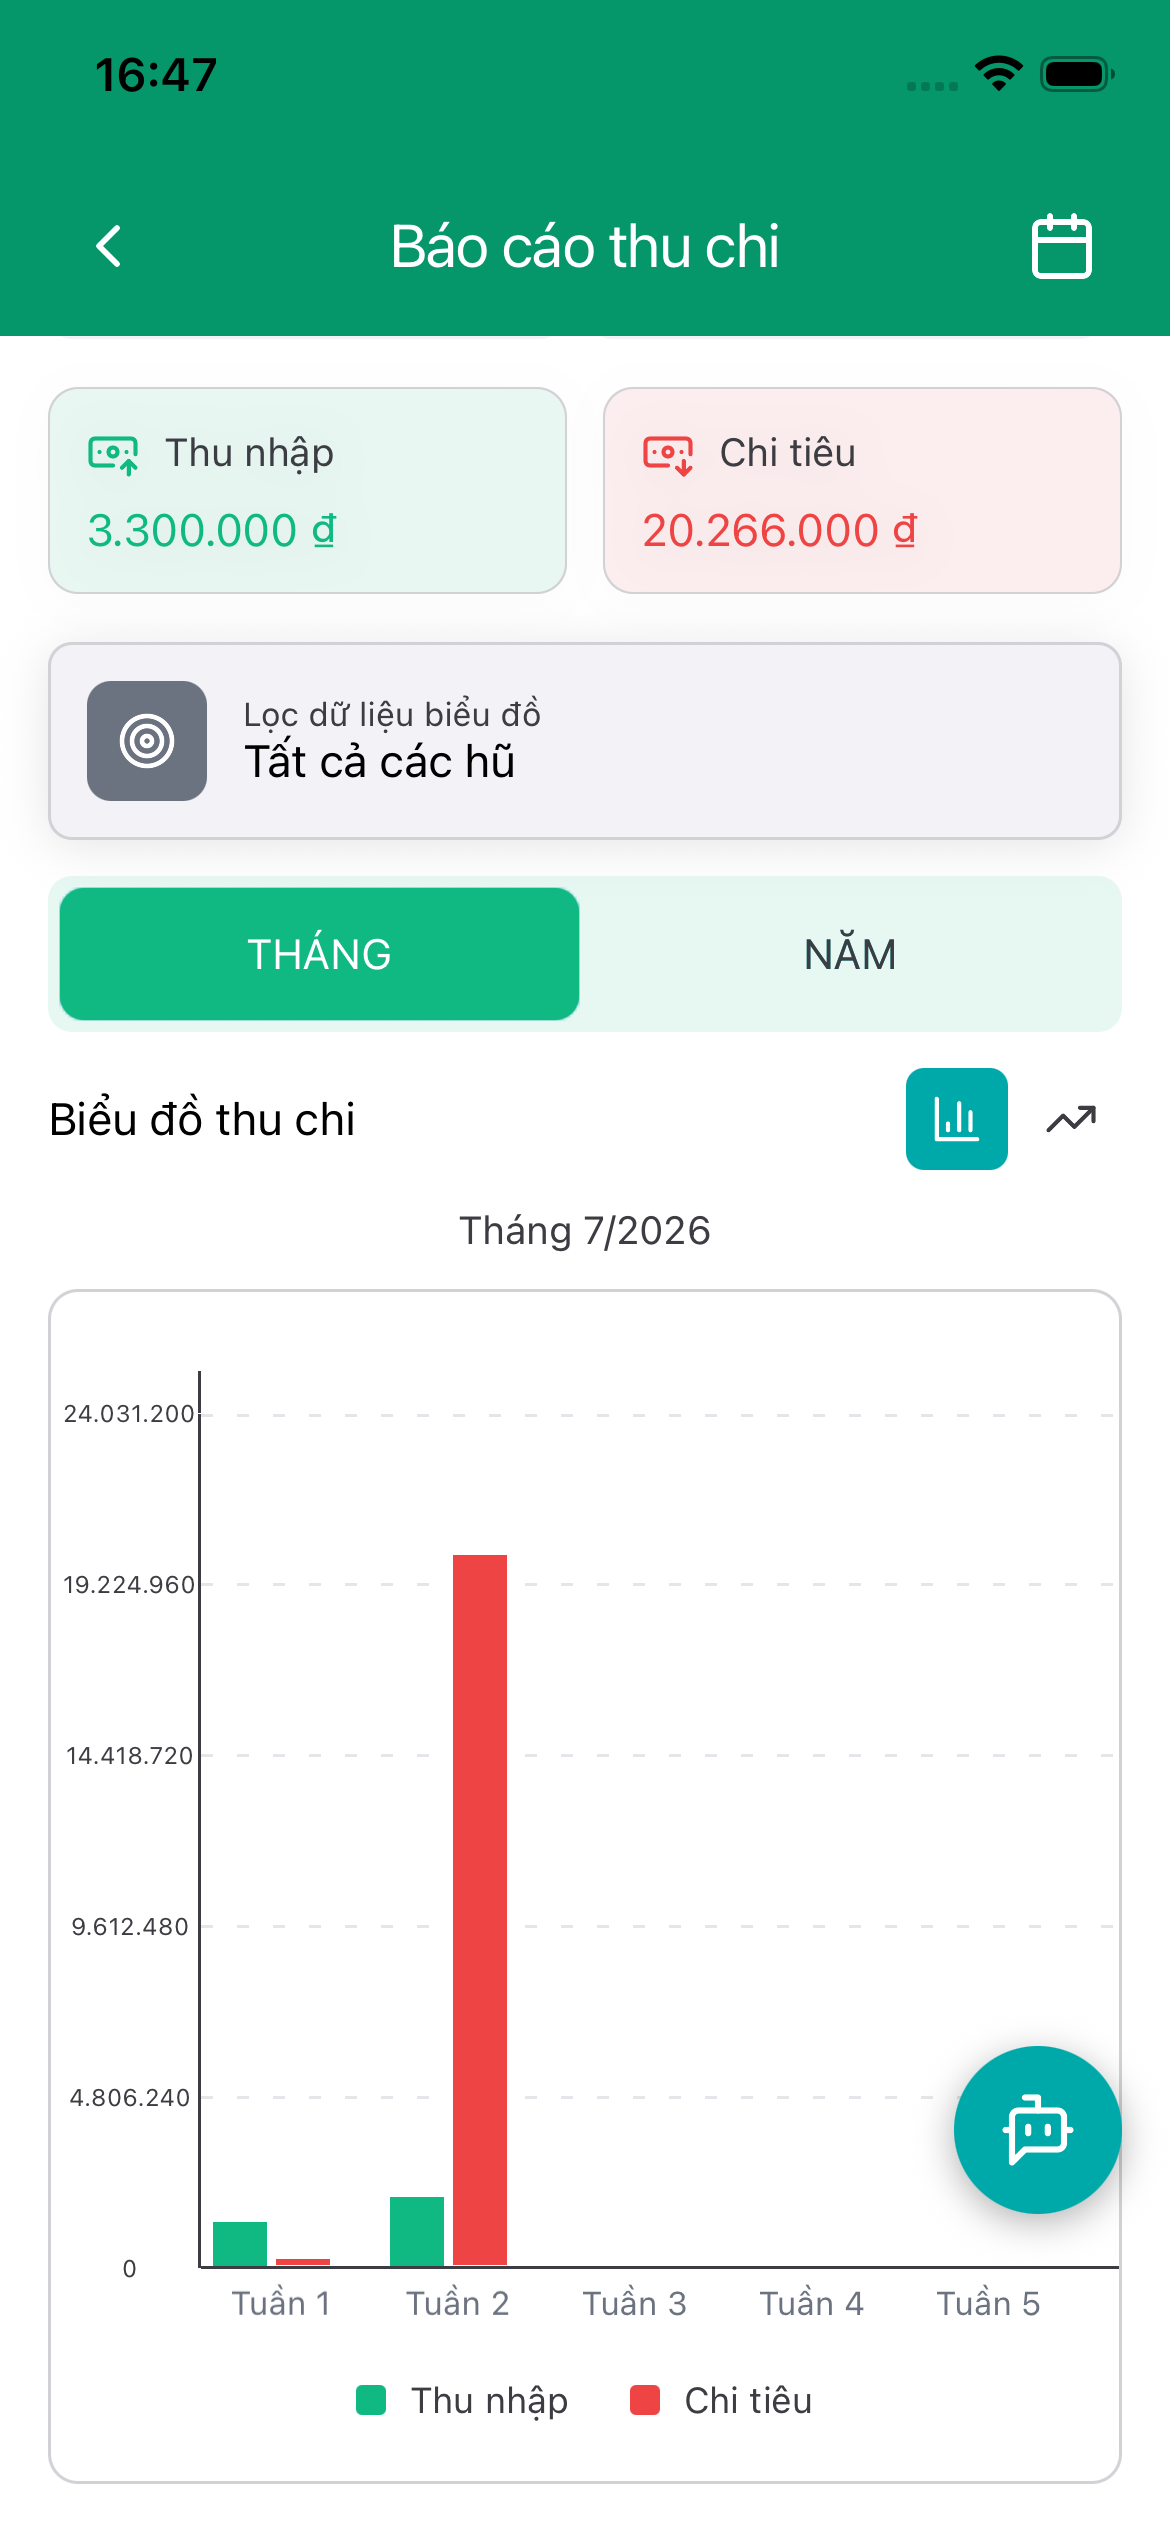
\includegraphics[width=\textwidth]{images/chapter4/mobile/financial-report-chart.png}%
        }{%
            \rectbox{Hình ảnh biểu đồ thu chi theo tuần trên báo cáo tài chính}
        }
        \caption{Biểu đồ thu chi theo tuần và AI Insights trên màn hình báo cáo}
        \label{fig:mobile-financial-report-chart}
    \end{minipage}
\end{figure}
\clearpage

\begin{figure}[H]
    \noindent\textbf{9.} \textbf{Gợi ý học bổng:} Màn hình này hiển thị danh sách các học bổng trực tuyến phù hợp nhất với sinh viên, được sắp xếp tự động dựa trên điểm tương thích hồ sơ (GPA, ngành học) của từng sinh viên.
    
    \vspace{0.2cm}
    \centering
    \begin{minipage}{0.44\textwidth}
        \centering
        \IfFileExists{images/chapter4/mobile/H5.14-1.png}{%
            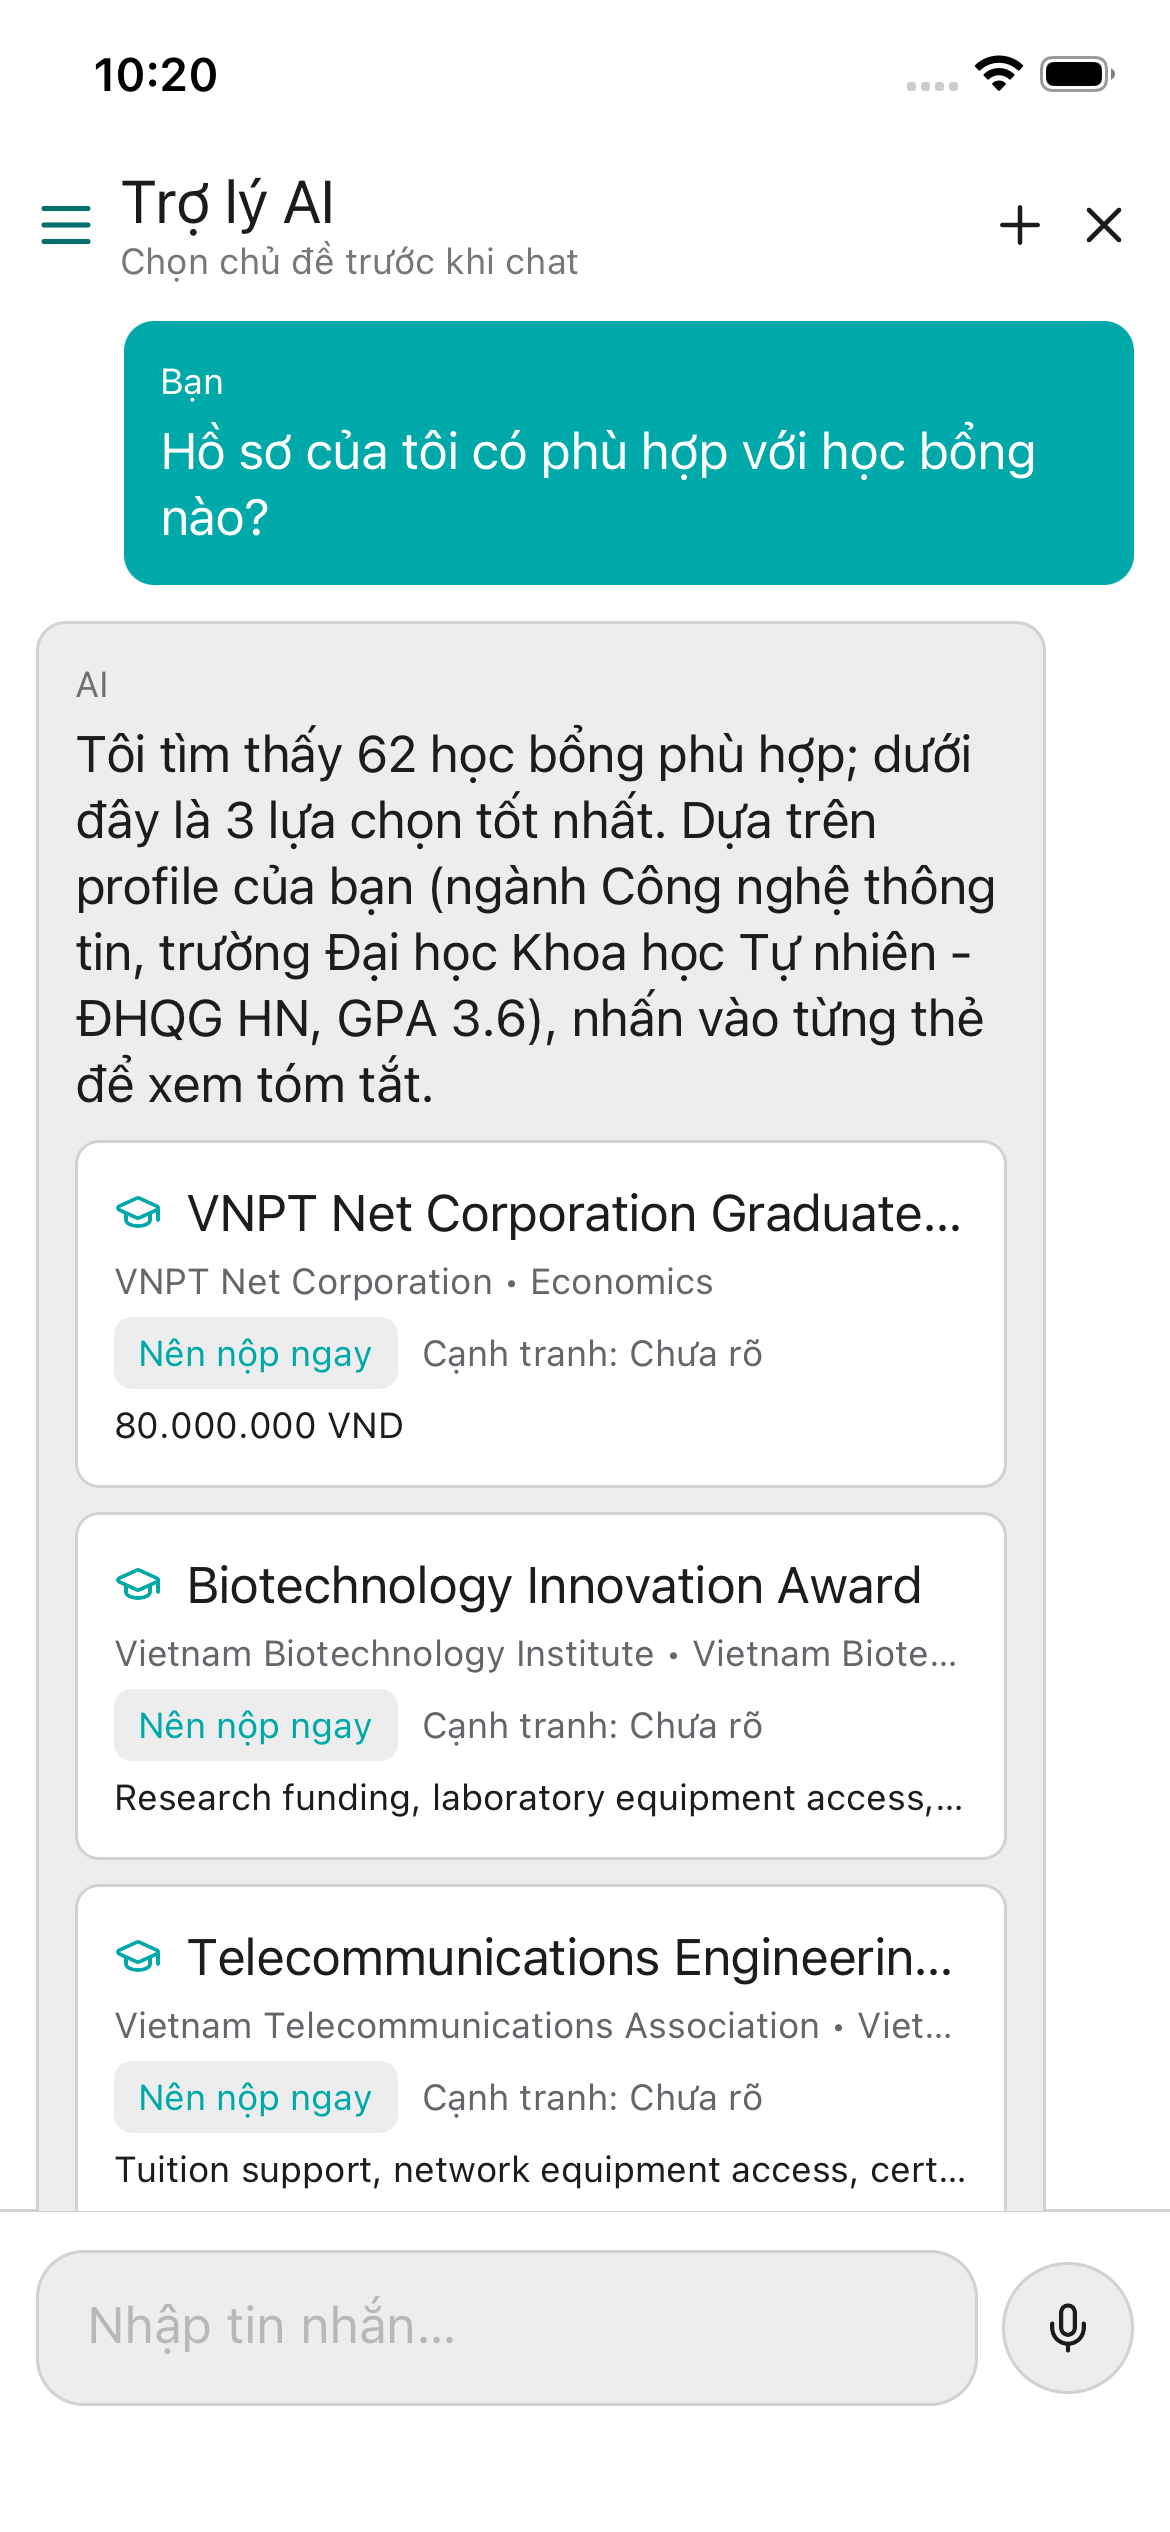
\includegraphics[width=\textwidth]{images/chapter4/mobile/H5.14-1.png}%
        }{%
            \rectbox{Gợi ý học bổng 1}
        }
        \centerline{(a) Danh sách gợi ý học bổng}
    \end{minipage}
    \hfill
    \begin{minipage}{0.44\textwidth}
        \centering
        \IfFileExists{images/chapter4/mobile/H5.14-2.png}{%
            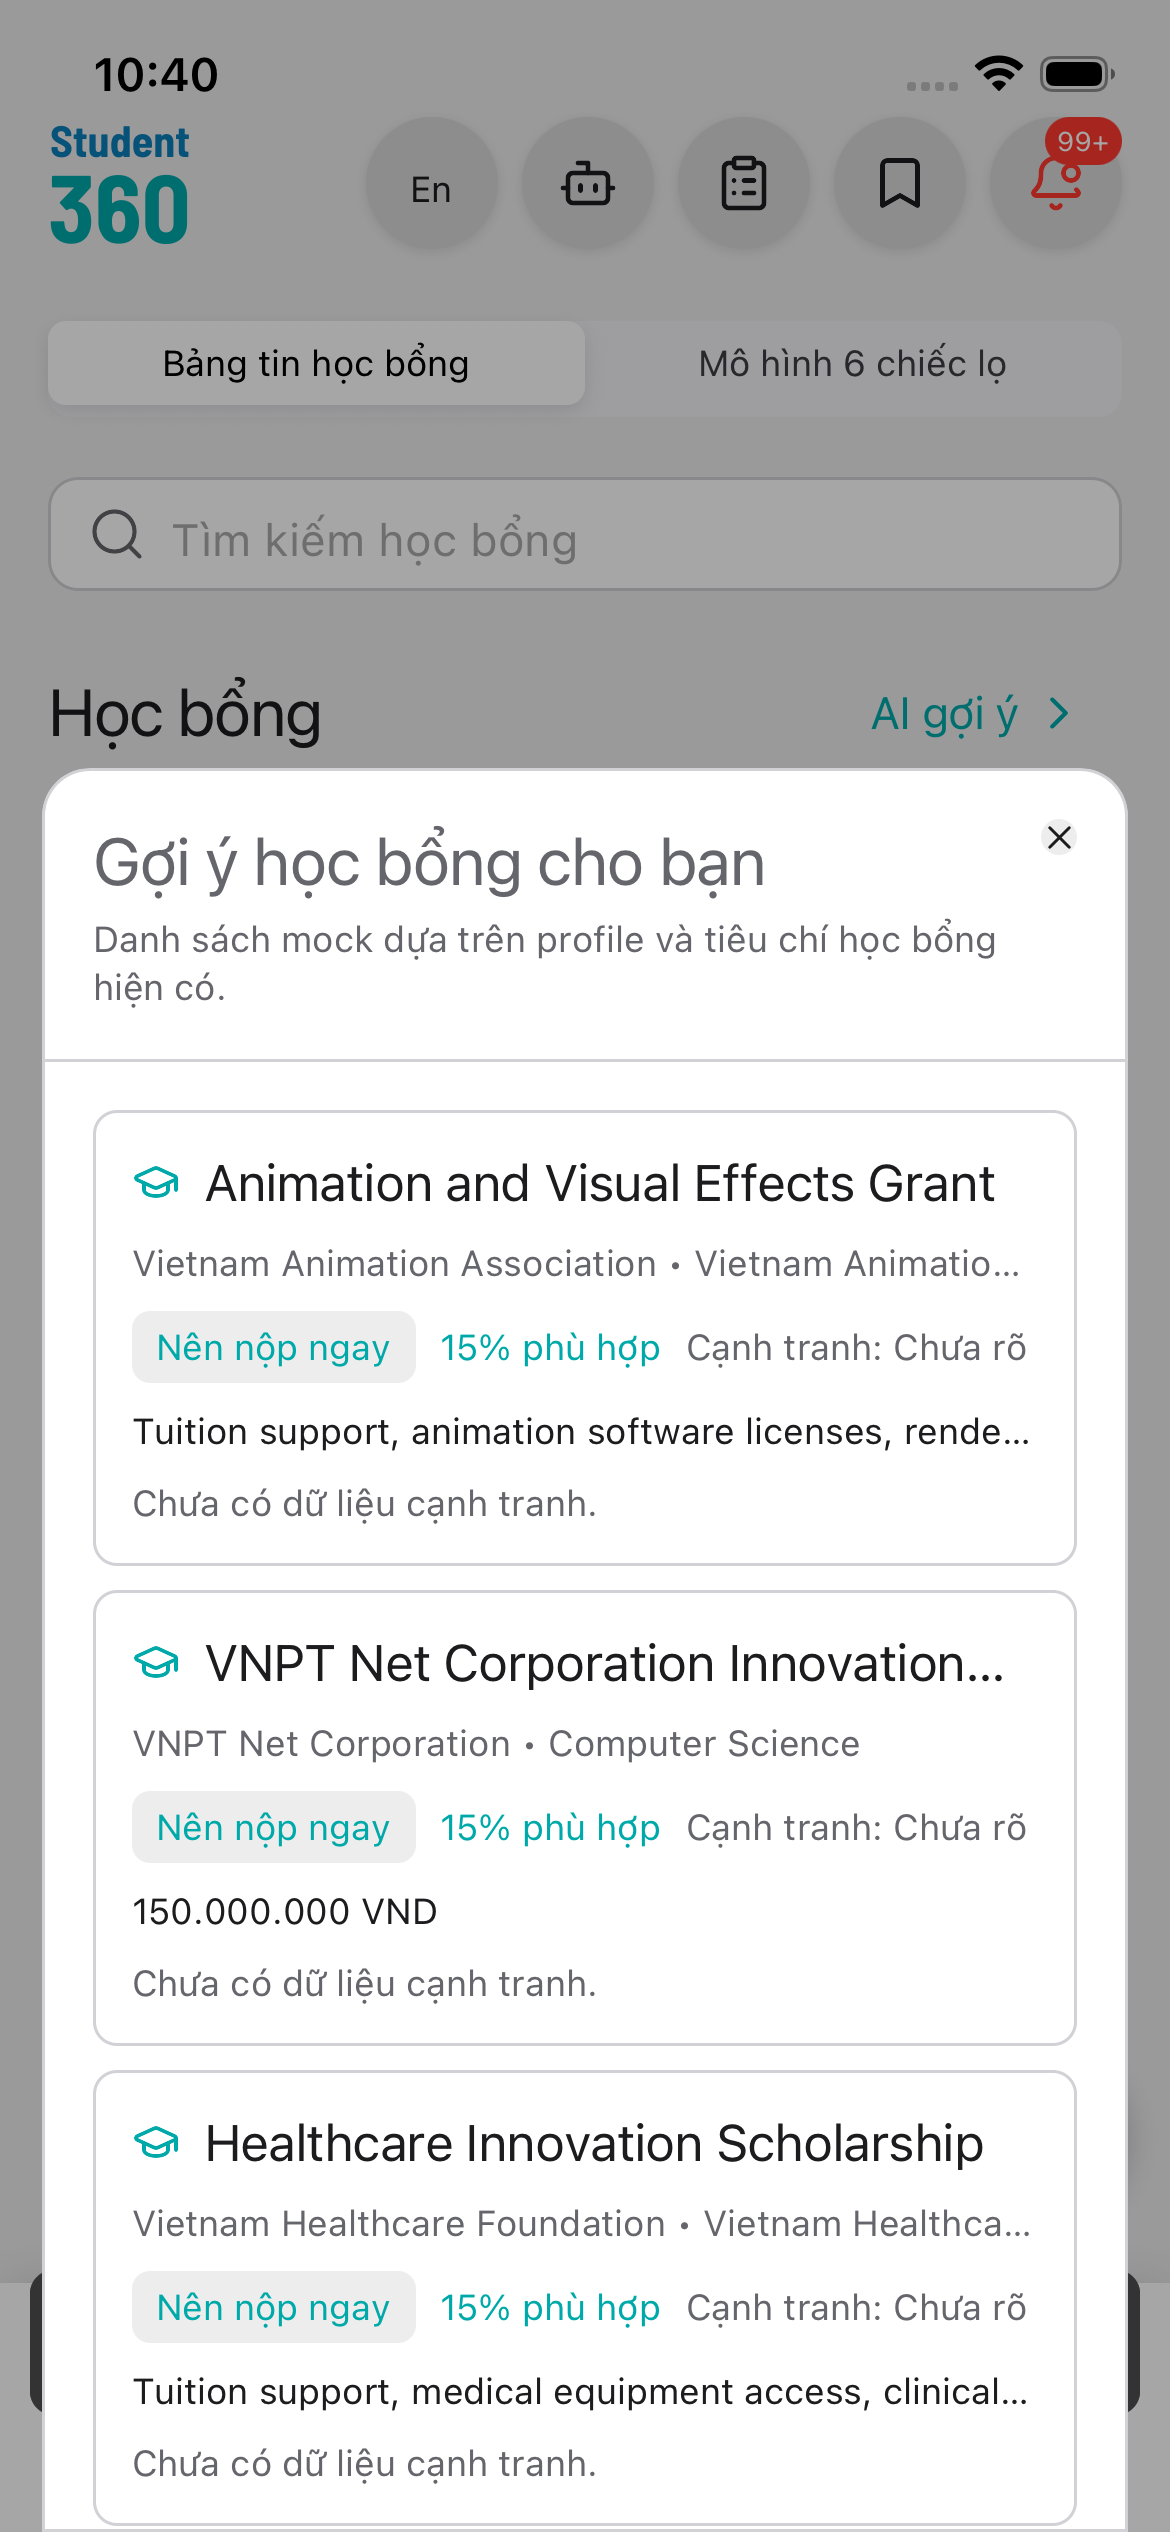
\includegraphics[width=\textwidth]{images/chapter4/mobile/H5.14-2.png}%
        }{%
            \rectbox{Gợi ý học bổng 2}
        }
        \centerline{(b) Chi tiết điểm khớp hồ sơ}
    \end{minipage}
    \caption{Giao diện gợi ý học bổng thông minh, xếp hạng theo điểm khớp hồ sơ}
    \label{fig:mobile-schol-match}
\end{figure}

\begin{figure}[H]
    \noindent\textbf{10.} \textbf{Chi tiết học bổng và Nộp hồ sơ:} Màn hình này hiển thị các thông tin chi tiết về học bổng (tiêu chuẩn, số lượng, giá trị và hạn nộp) và biểu mẫu nộp hồ sơ đăng ký. Sinh viên có thể tải lên các file tài liệu minh chứng (PDF/hình ảnh) trực tiếp từ điện thoại.
    
    \vspace{0.2cm}
    \centering
    \begin{minipage}{0.44\textwidth}
        \centering
        \IfFileExists{images/chapter4/mobile/scholarship-apply.png}{%
            
\includegraphics[width=\textwidth]{images/chapter4/mobile/scholarship-apply.png}%
        }{%
            \rectbox{Hình ảnh màn hình chi tiết học bổng trên Mobile}
        }
        \caption{Giao diện chi tiết học bổng trên thiết bị di động}
        \label{fig:mobile-scholarship-apply}
    \end{minipage}
    \hfill
    \begin{minipage}{0.44\textwidth}
        \centering
        \IfFileExists{images/chapter4/mobile/scholarship-apply-form.png}{%
            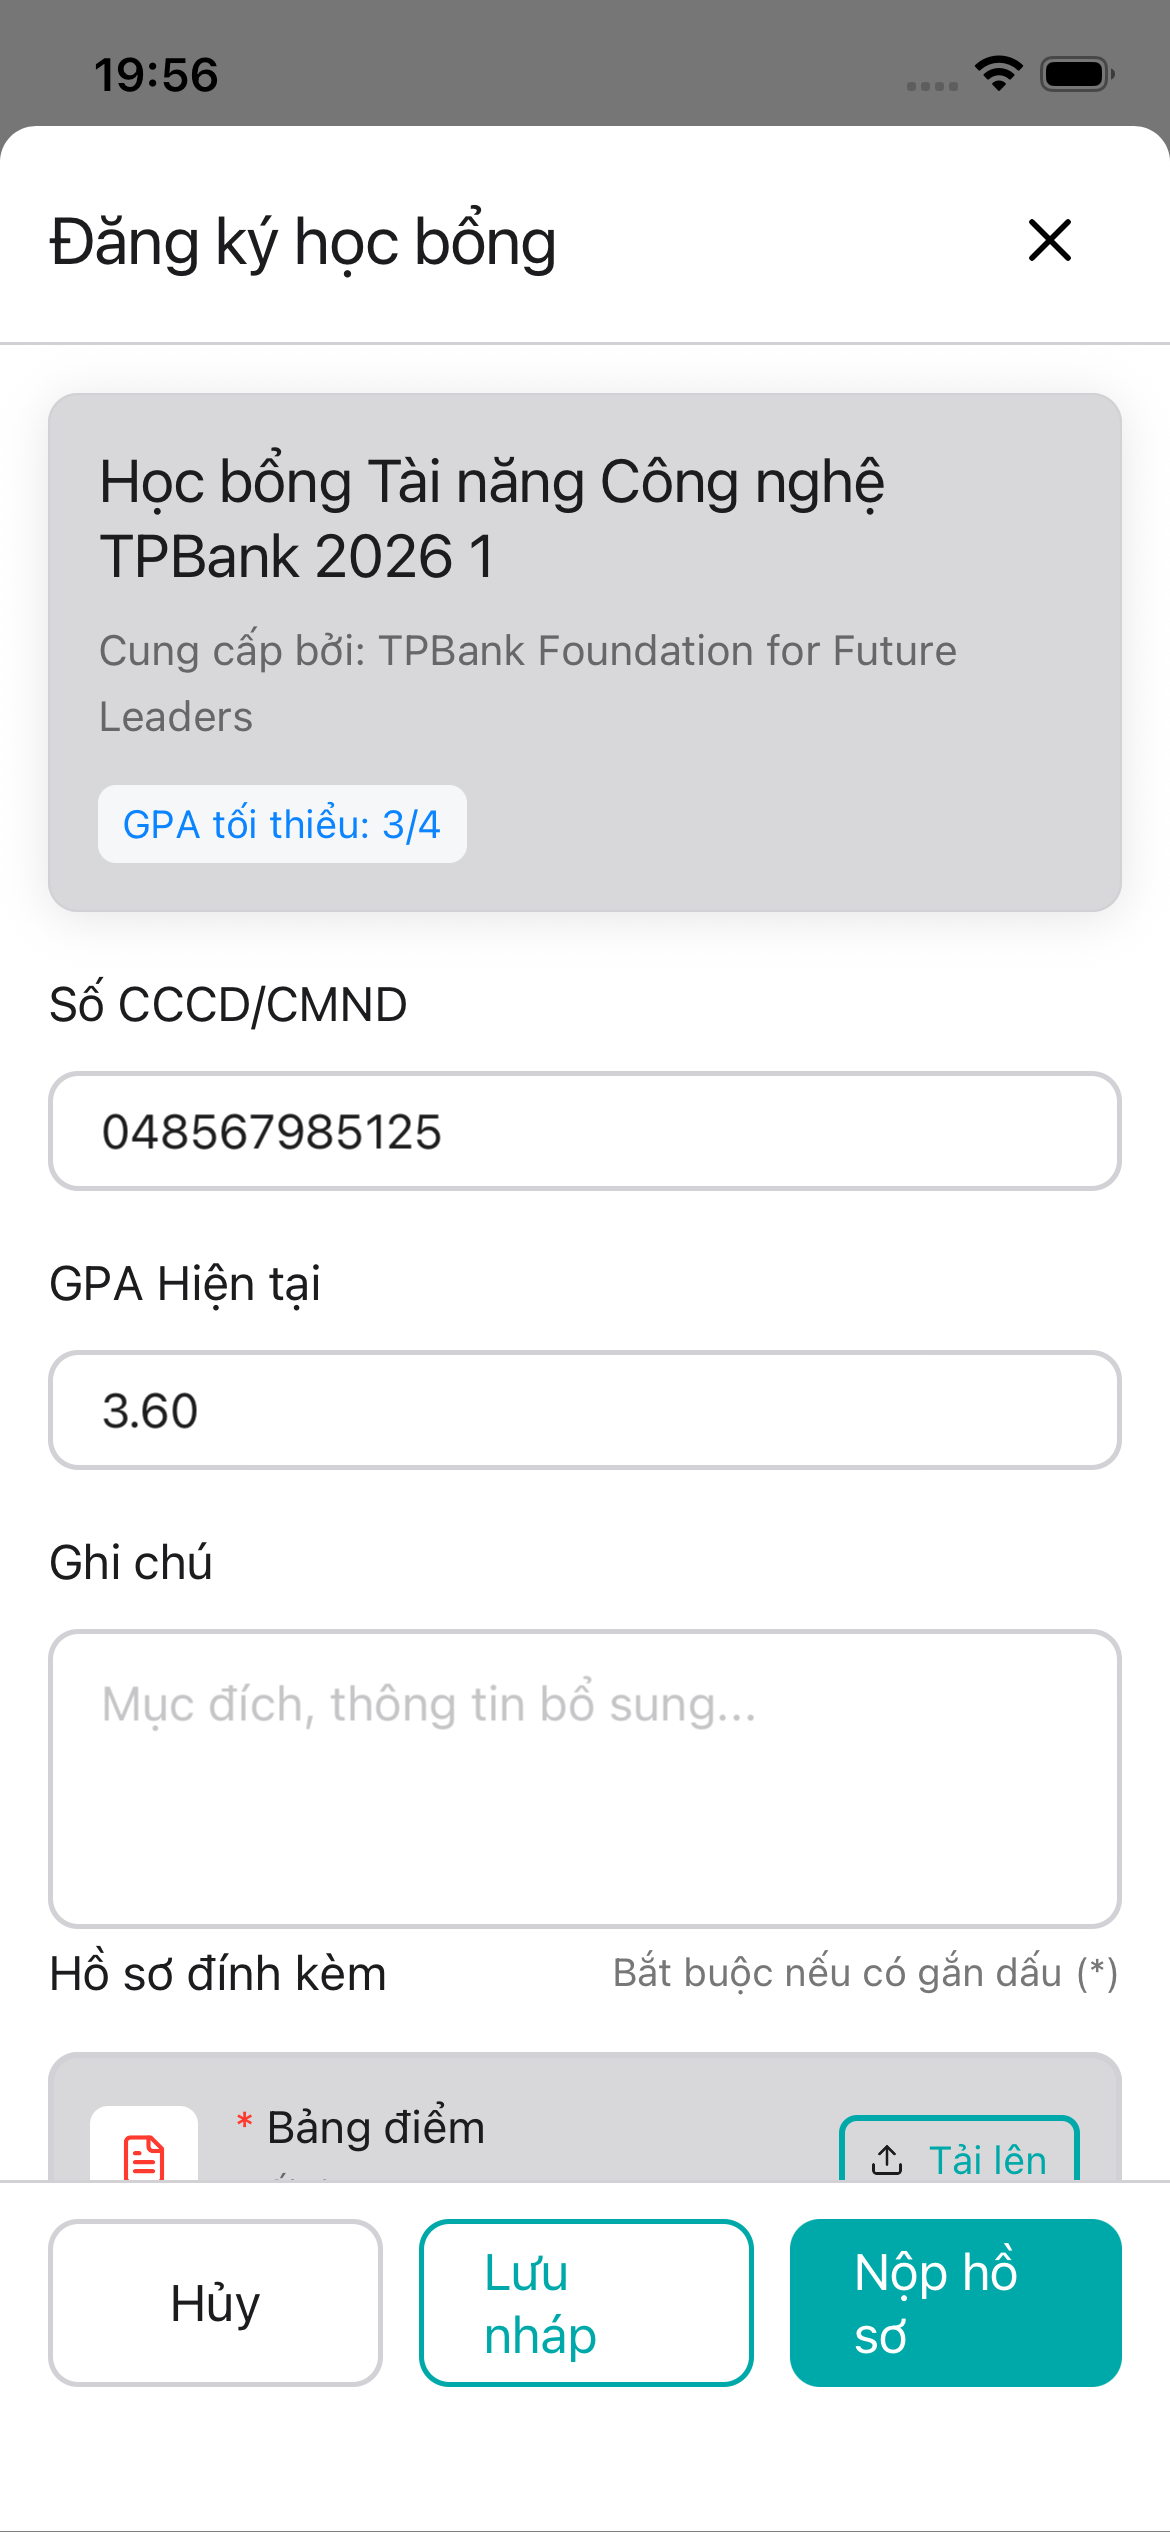
\includegraphics[width=\textwidth]{images/chapter4/mobile/scholarship-apply-form.png}%
        }{%
            \rectbox{Hình ảnh form đăng ký nộp hồ sơ học bổng trên Mobile}
        }
        \caption{Biểu mẫu đăng ký và nộp hồ sơ học bổng}
        \label{fig:mobile-scholarship-apply-form}
    \end{minipage}
\end{figure}
\clearpage

\begin{figure}[H]
    \noindent\textbf{11.} \textbf{Bảng điểm sinh viên:} Màn hình này hiển thị chi tiết kết quả học tập của sinh viên, bao gồm điểm trung bình tích lũy (GPA), tổng số tín chỉ đạt được và tiến độ đạt mục tiêu tốt nghiệp.
    
    \vspace{0.2cm}
    \centering
    \begin{minipage}{0.44\textwidth}
        \centering
        \IfFileExists{images/chapter4/mobile/gradebook-dashboard.png}{%
            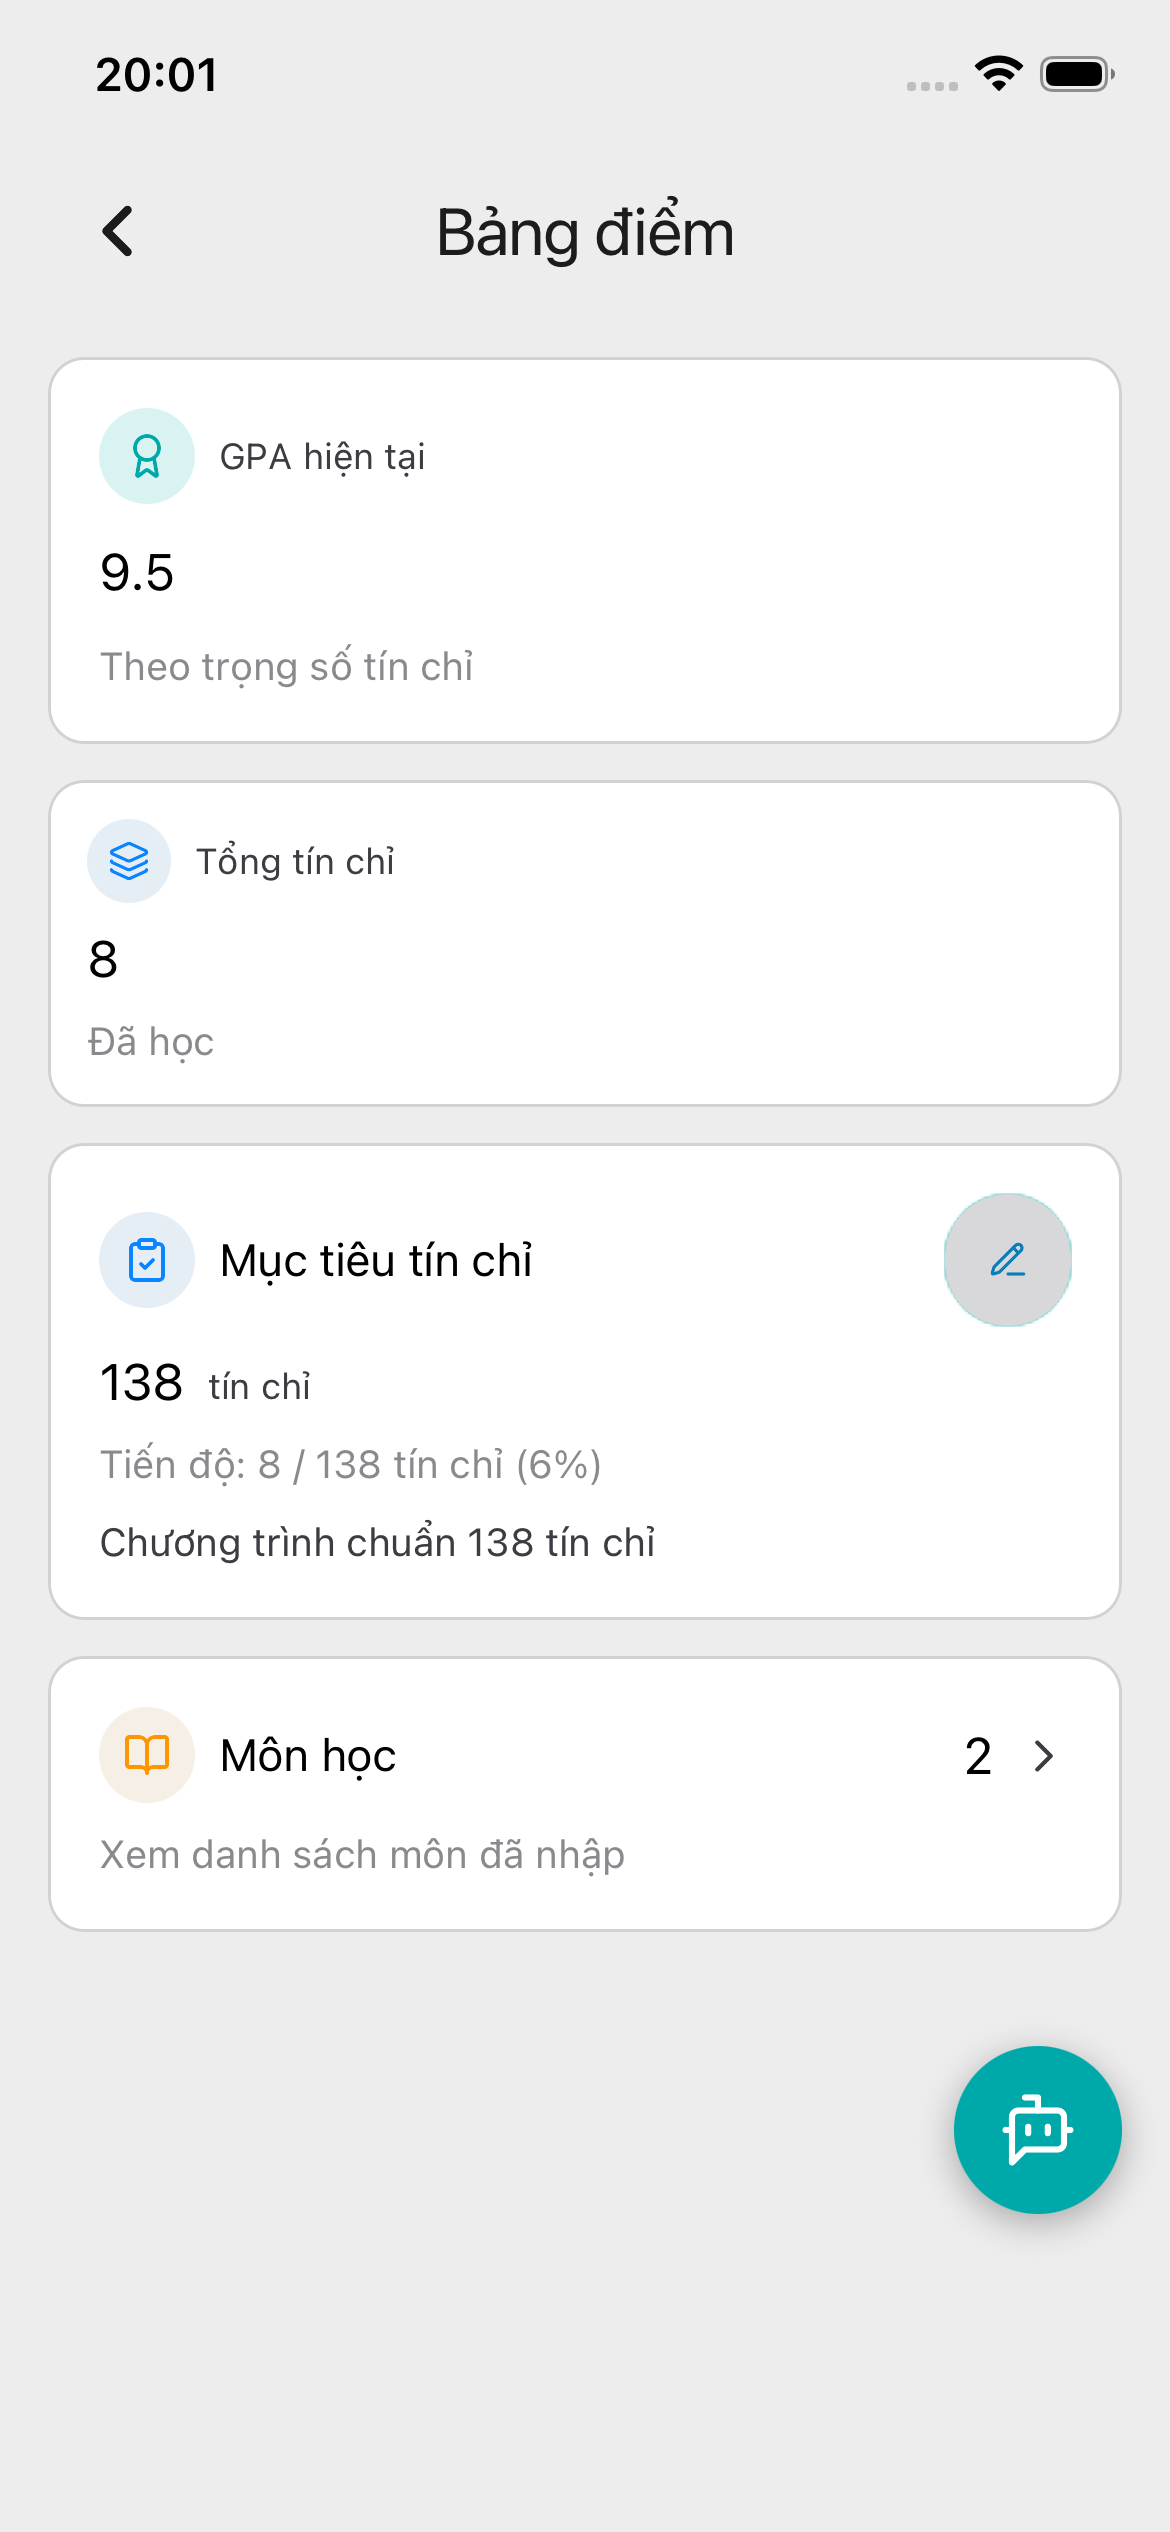
\includegraphics[width=\textwidth]{images/chapter4/mobile/gradebook-dashboard.png}%
        }{%
            \rectbox{Màn hình dashboard bảng điểm, GPA và mục tiêu tín chỉ trên Mobile}
        }
        \caption{Giao diện bảng điểm và tiến độ tín chỉ của sinh viên}
        \label{fig:mobile-gradebook-dashboard}
    \end{minipage}
    \hfill
    \begin{minipage}{0.44\textwidth}
        \centering
        \IfFileExists{images/chapter4/mobile/gradebook-courses.png}{%
            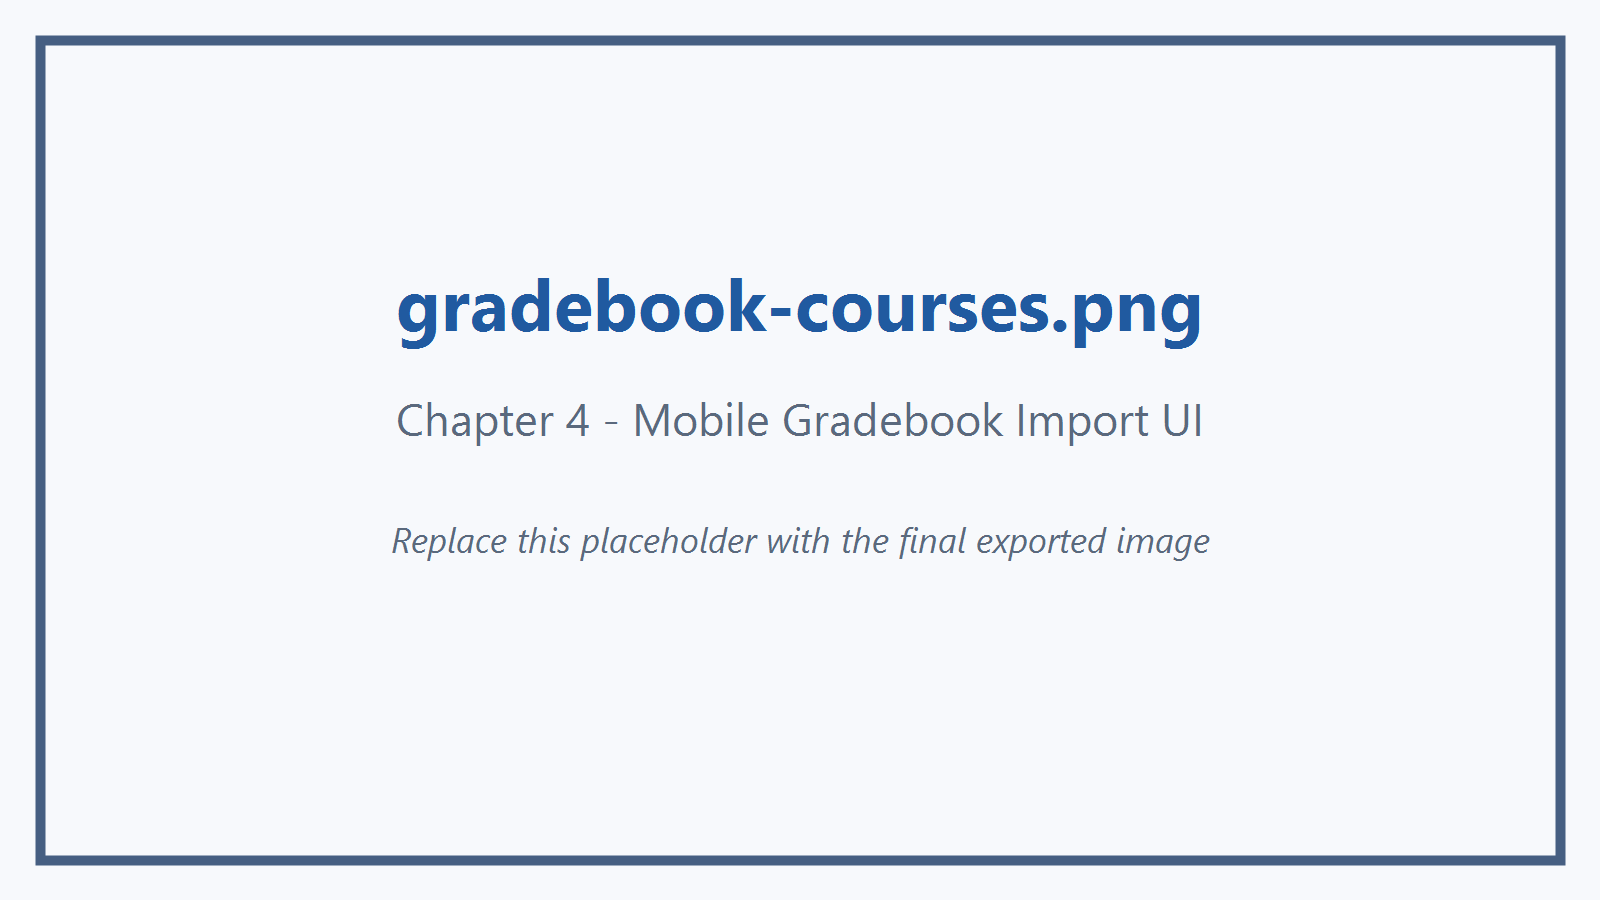
\includegraphics[width=\textwidth]{images/chapter4/mobile/gradebook-courses.png}%
        }{%
            \rectbox{Màn hình thêm môn học và import bảng điểm TXT/CSV trên Mobile}
        }
        \caption{Giao diện nhập và import điểm sinh viên}
        \label{fig:mobile-gradebook-courses}
    \end{minipage}
\end{figure}

\begin{figure}[H]
    \noindent\textbf{12.} \textbf{Nhập môn và Import bảng điểm:} Màn hình này cho phép sinh viên nhanh chóng cập nhật bảng điểm bằng cách chọn trực tiếp môn học từ danh mục đào tạo chuẩn của trường đối tác, hoặc tải lên tệp văn bản (TXT/CSV) kết quả học tập để hệ thống tự động trích xuất điểm và số tín chỉ.

    \vspace{0.2cm}
    \centering
    \begin{minipage}{0.44\textwidth}
        \centering
        \IfFileExists{images/chapter4/mobile/H5.12-1.png}{%
            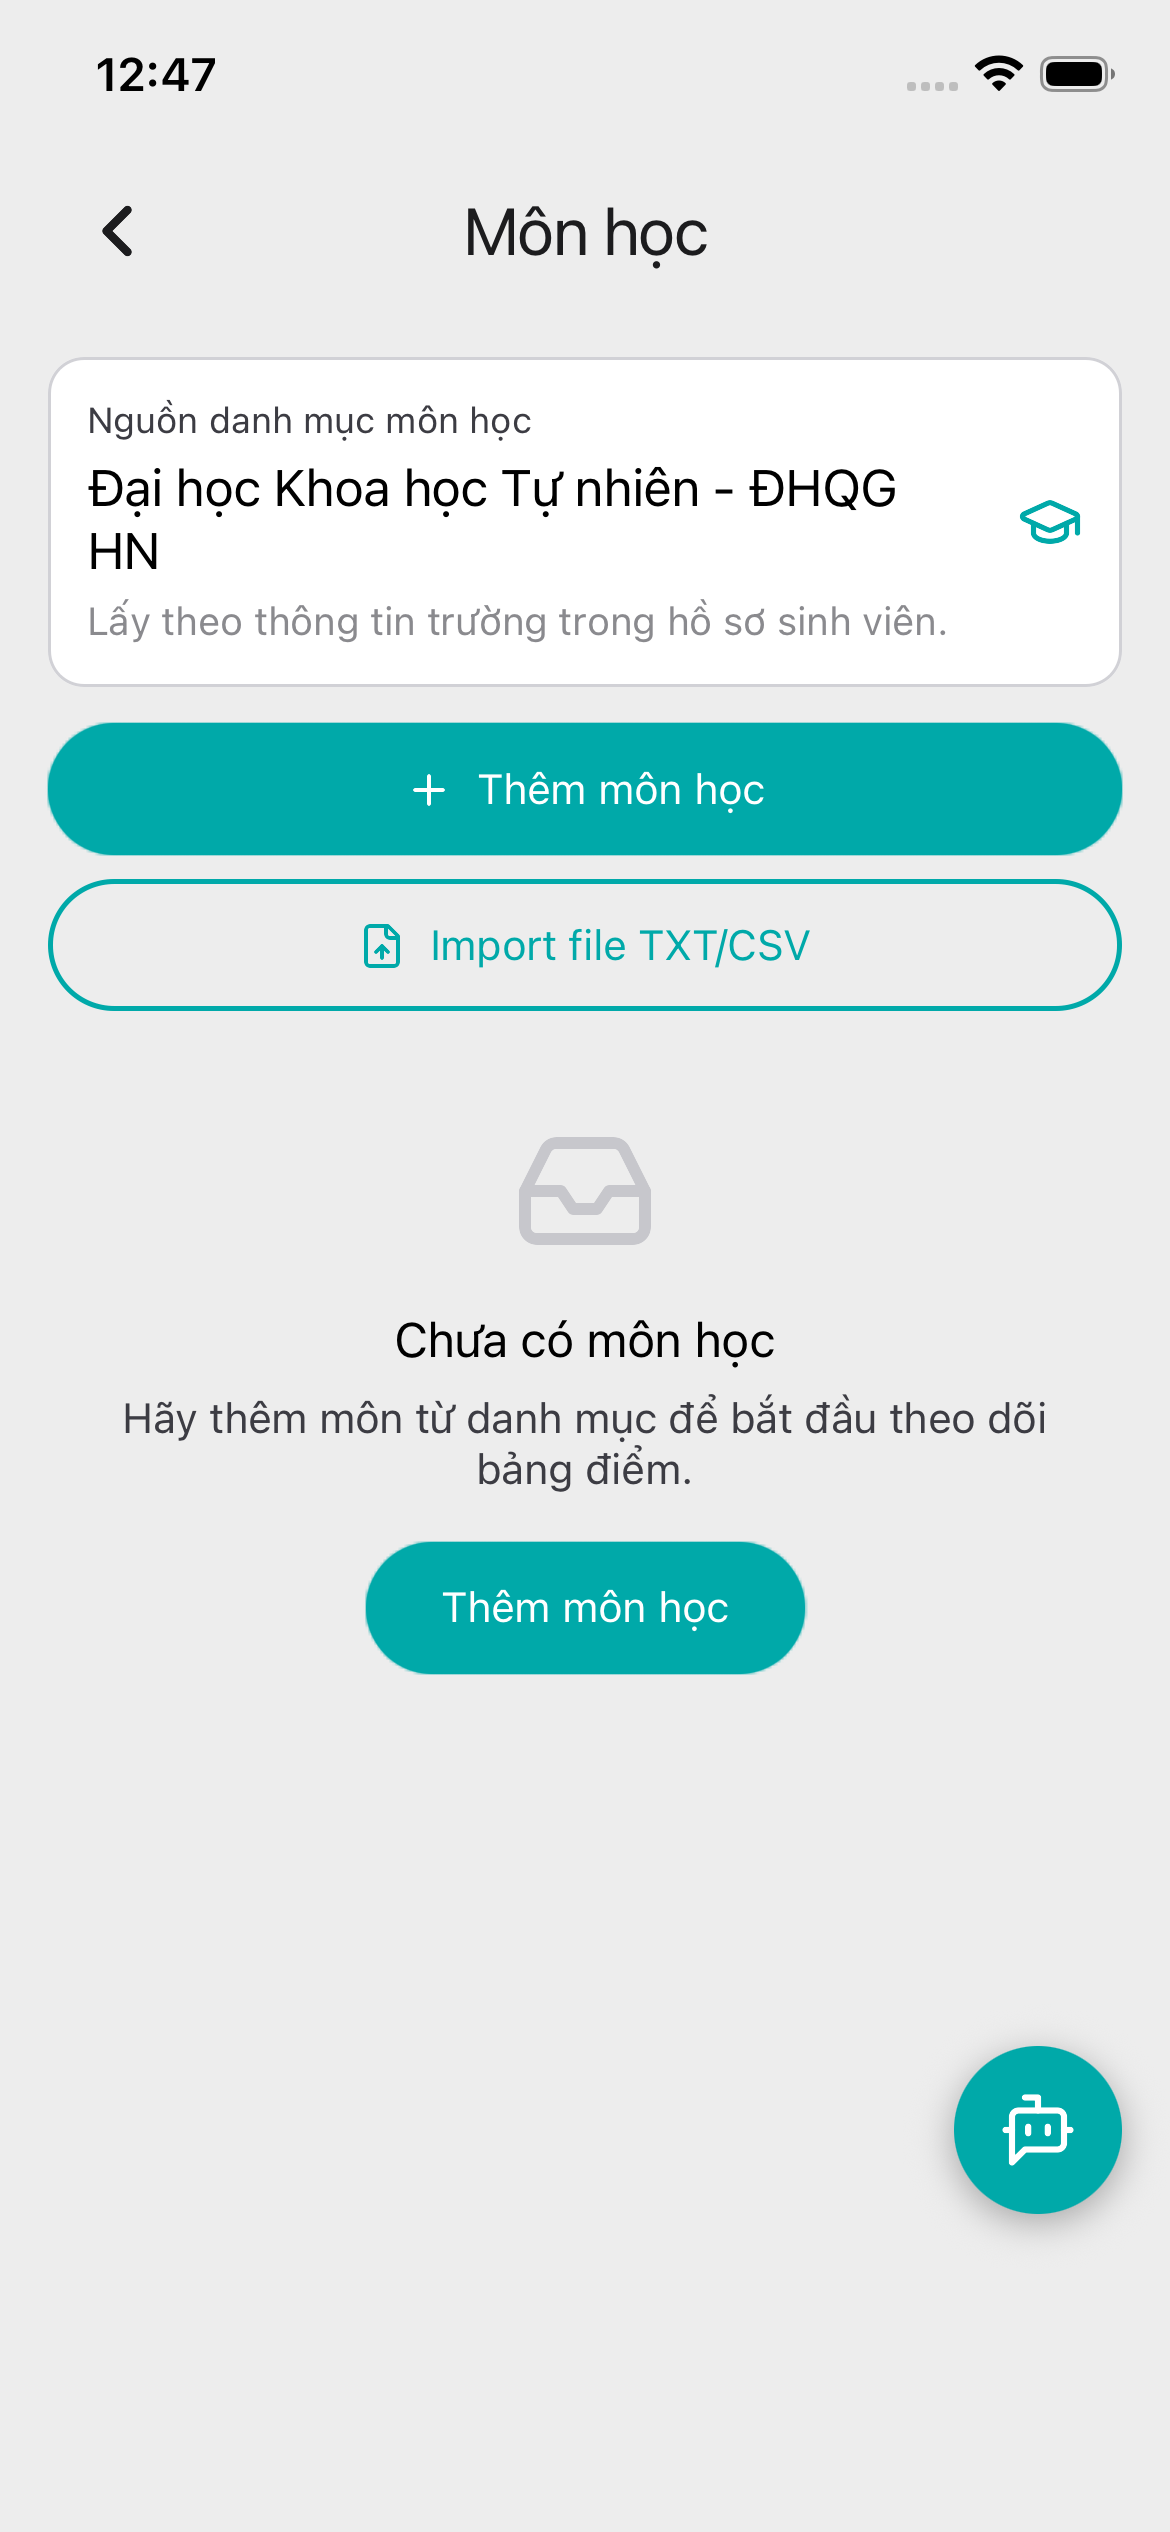
\includegraphics[width=\textwidth]{images/chapter4/mobile/H5.12-1.png}%
        }{%
            \rectbox{Màn hình chọn môn học từ danh mục chuẩn}
        }
        \caption{Giao diện thêm môn học và import bảng điểm}
        \label{fig:mobile-gradebook-add-subject}
    \end{minipage}
    \hfill
\end{figure}
\clearpage

\subsection{Webadmin quản trị hệ thống}
Giao diện quản trị Webadmin được xây dựng bằng React JS kết hợp Material UI (MUI), tối ưu cho việc hiển thị bảng dữ liệu lớn và xử lý quy trình phê duyệt.

\begin{enumerate}
    \item \textbf{Quản lý Trường đối tác:} Màn hình này cho phép quản trị viên xem, thêm mới hoặc điều chỉnh danh sách các trường đại học liên kết trong hệ thống để quản trị danh mục đào tạo.
    
    \begin{figure}[H]
        \centering
        \IfFileExists{images/chapter4/webadmin/universities.png}{%
            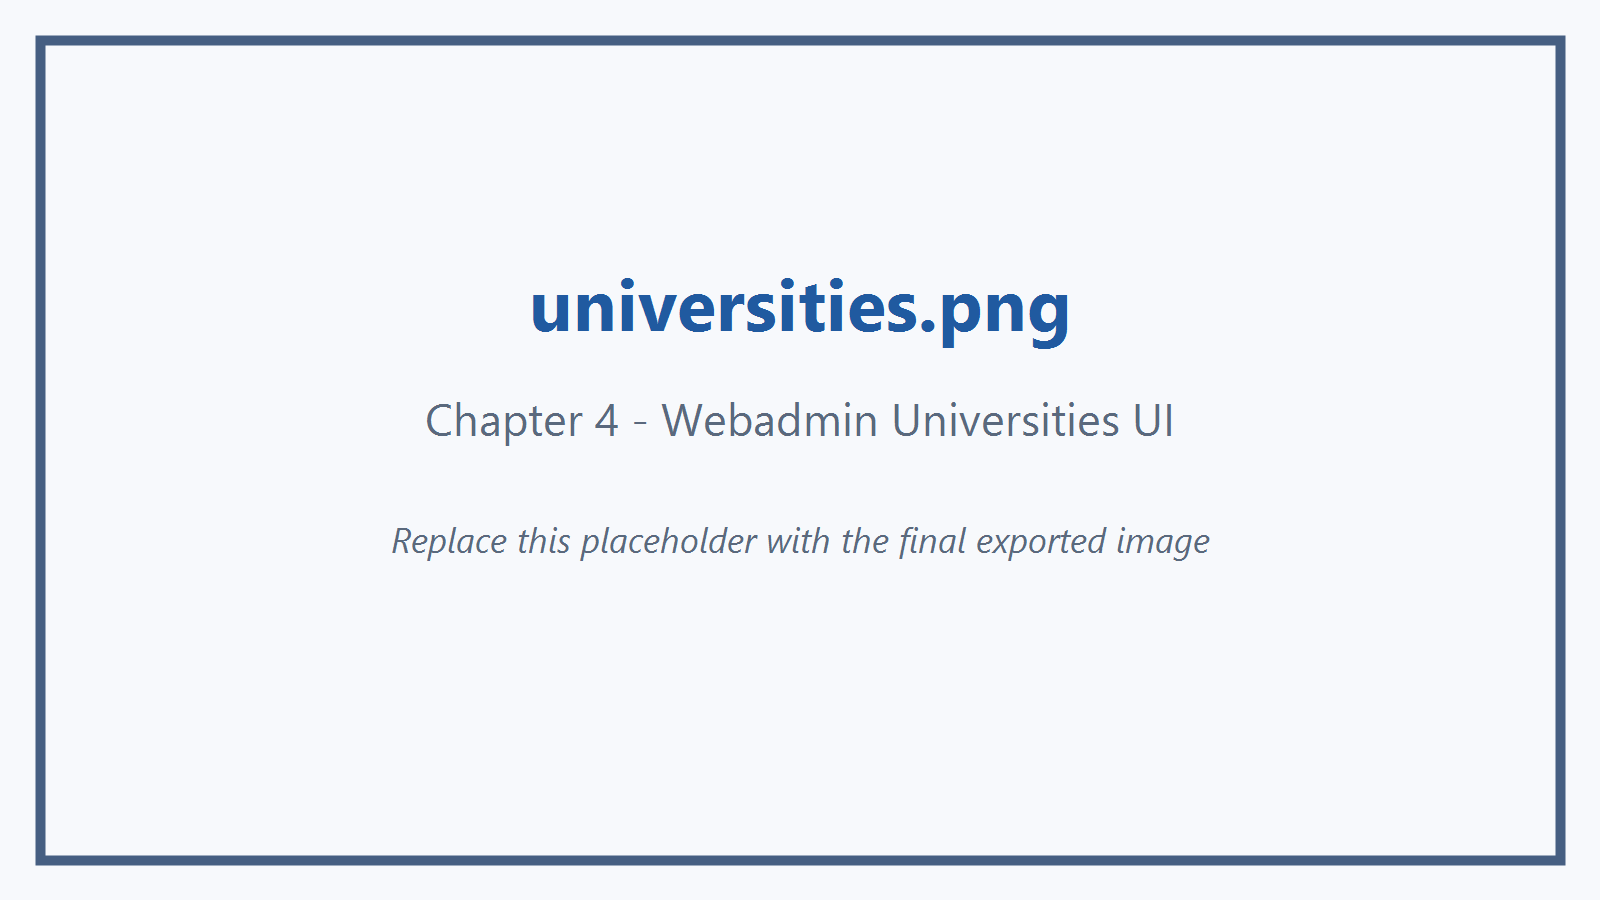
\includegraphics[width=0.85\textwidth]{images/chapter4/webadmin/universities.png}%
        }{%
            \rectbox{Màn hình danh sách trường đại học trên Webadmin}
        }
        \caption{Giao diện quản lý danh mục trường đại học (thêm/sửa qua modal, tìm kiếm theo từ khóa)}
        \label{fig:webadmin-universities}
    \end{figure}
    \clearpage

    \item \textbf{Quản lý Môn học và Khoa:} Màn hình này dùng để quản lý chi tiết danh mục khoa, chương trình đào tạo và môn học tương ứng của từng trường đại học đối tác nhằm phục vụ cho chức năng quản lý bảng điểm của sinh viên.
    
    \begin{figure}[H]
        \centering
        \IfFileExists{images/chapter4/webadmin/subjects-programs.png}{%
            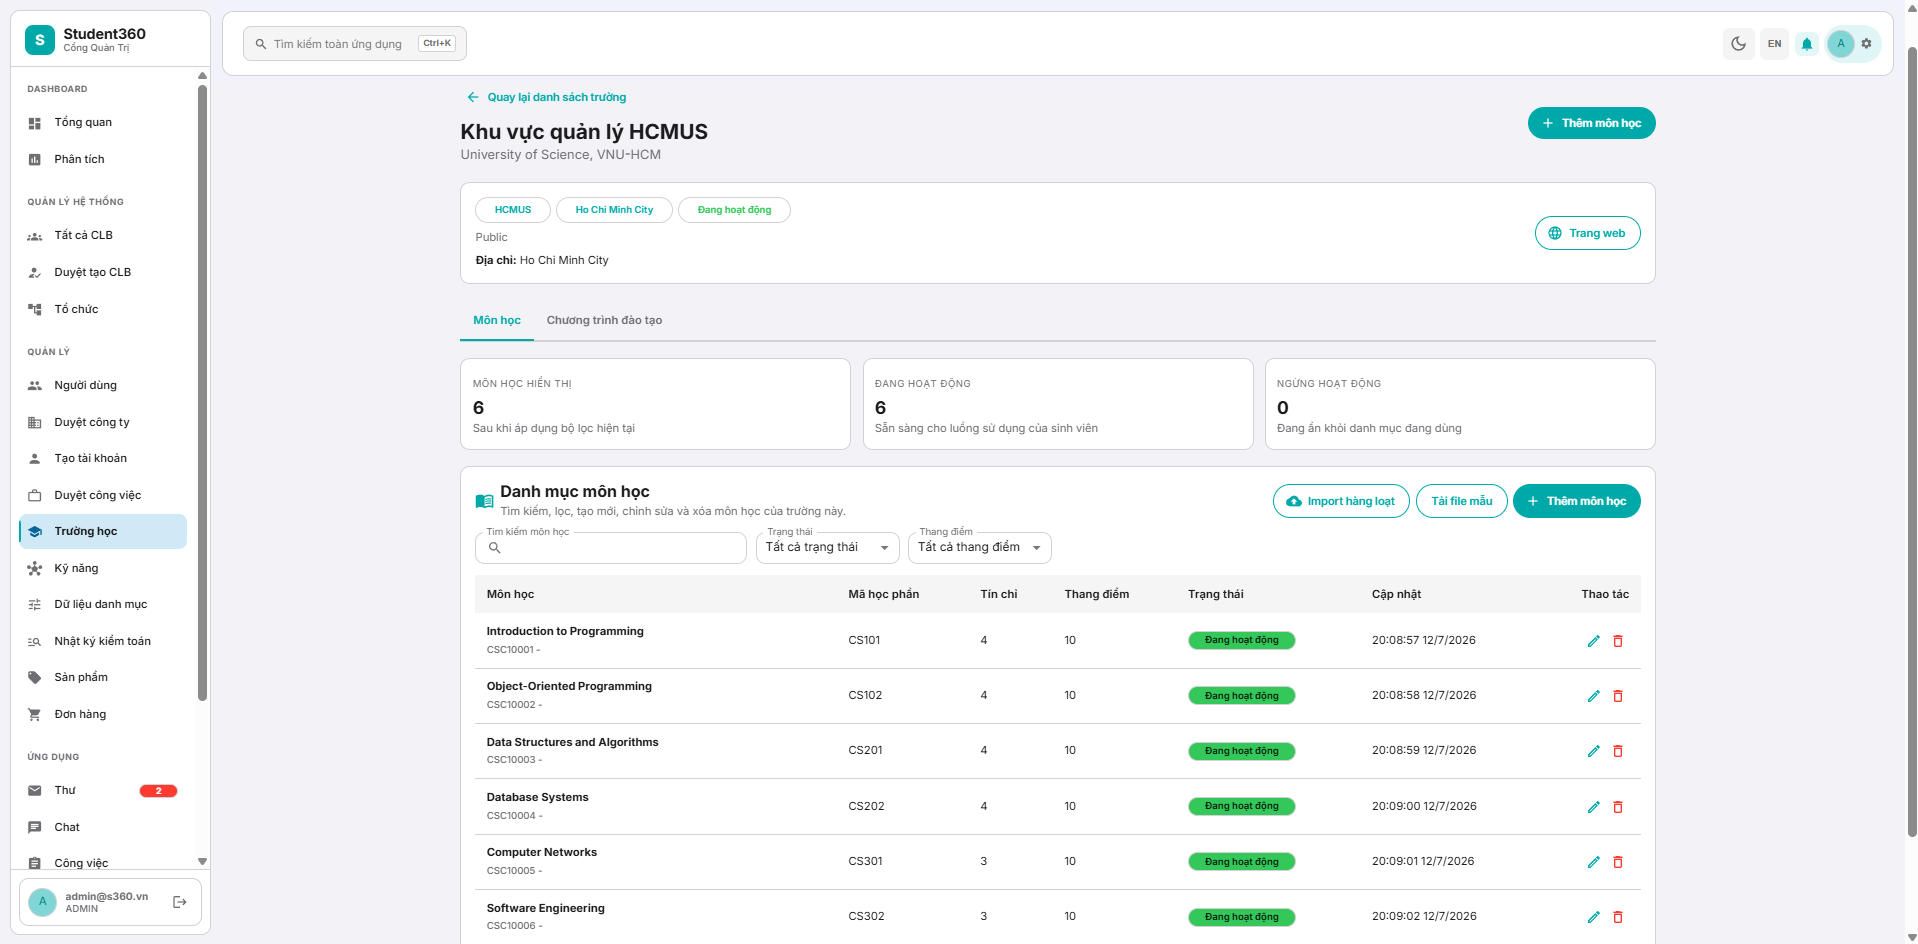
\includegraphics[width=0.85\textwidth,height=0.35\textheight,keepaspectratio]{images/chapter4/webadmin/subjects-programs.png}%
        }{%
            \rectbox{Màn hình quản lý môn học theo trường}
        }

        \vspace{0.4cm}

        \IfFileExists{images/chapter4/webadmin/training-programs.png}{%
            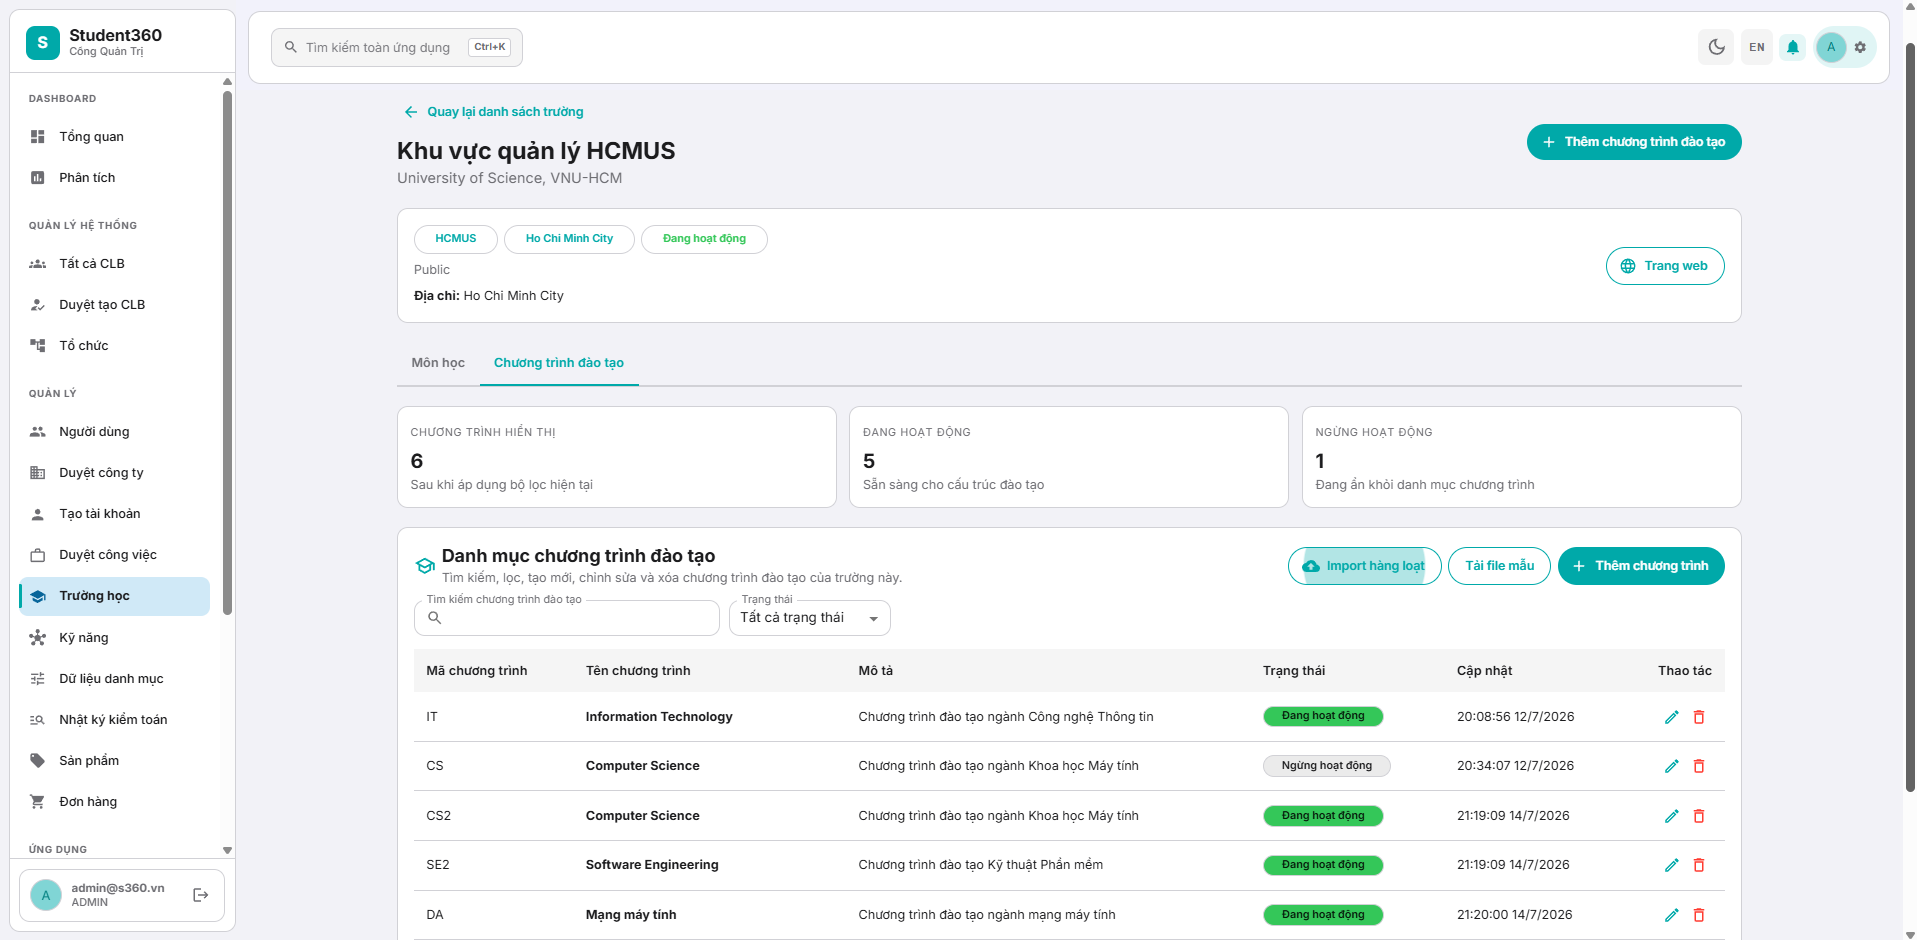
\includegraphics[width=0.85\textwidth,height=0.35\textheight,keepaspectratio]{images/chapter4/webadmin/training-programs.png}%
        }{%
            \rectbox{Màn hình quản lý khoa/chương trình đào tạo theo trường}
        }
        \caption{Giao diện quản lý môn học và khoa/chương trình đào tạo (hỗ trợ bulk import)}
        \label{fig:webadmin-subjects-programs}
    \end{figure}
    \clearpage

    \item \textbf{Danh sách Học bổng:} Màn hình này giúp các nhà tài trợ theo dõi danh sách toàn bộ các chương trình học bổng do mình tài trợ, cũng như tổng hợp số lượng hồ sơ đã ứng tuyển để tiến hành chấm điểm phê duyệt.
    
    \begin{figure}[H]
        \centering
        \IfFileExists{images/chapter4/webadmin/scholarships-list.png}{%
            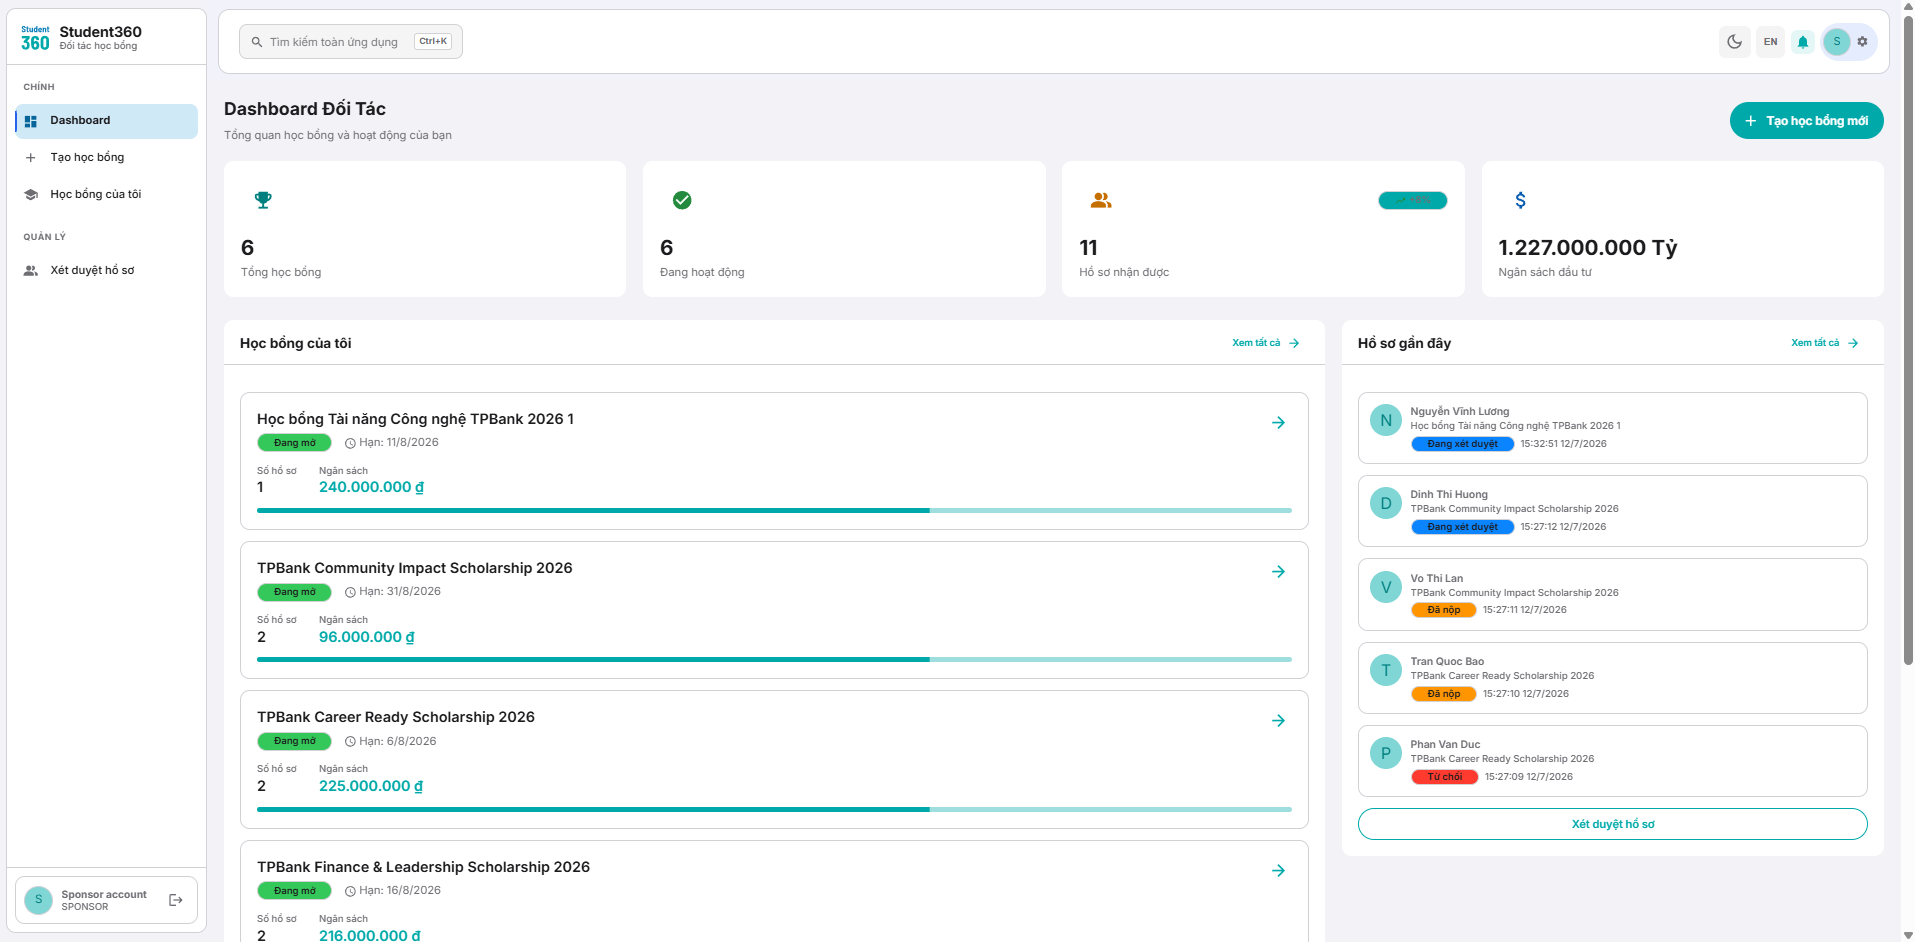
\includegraphics[width=0.85\textwidth]{images/chapter4/webadmin/scholarships-list.png}%
        }{%
            \rectbox{Màn hình danh sách Học bổng trên Webadmin}
        }
        \caption{Giao diện quản lý danh sách Học bổng, kèm thống kê tiến độ ứng tuyển}
        \label{fig:webadmin-scholarships-list}
    \end{figure}
    \clearpage

    \item \textbf{Tạo và Thiết lập Học bổng:} Màn hình này cung cấp biểu mẫu nhiều bước cho nhà tài trợ để xuất bản chương trình học bổng mới, thiết lập thông tin chung, giá trị giải thưởng và các tiêu chí lọc hồ sơ (như GPA tối thiểu, ngành học yêu cầu).
    
    \begin{figure}[H]
        \centering
        \IfFileExists{images/chapter4/webadmin/sponsor-create-scholarship-1.png}{%
            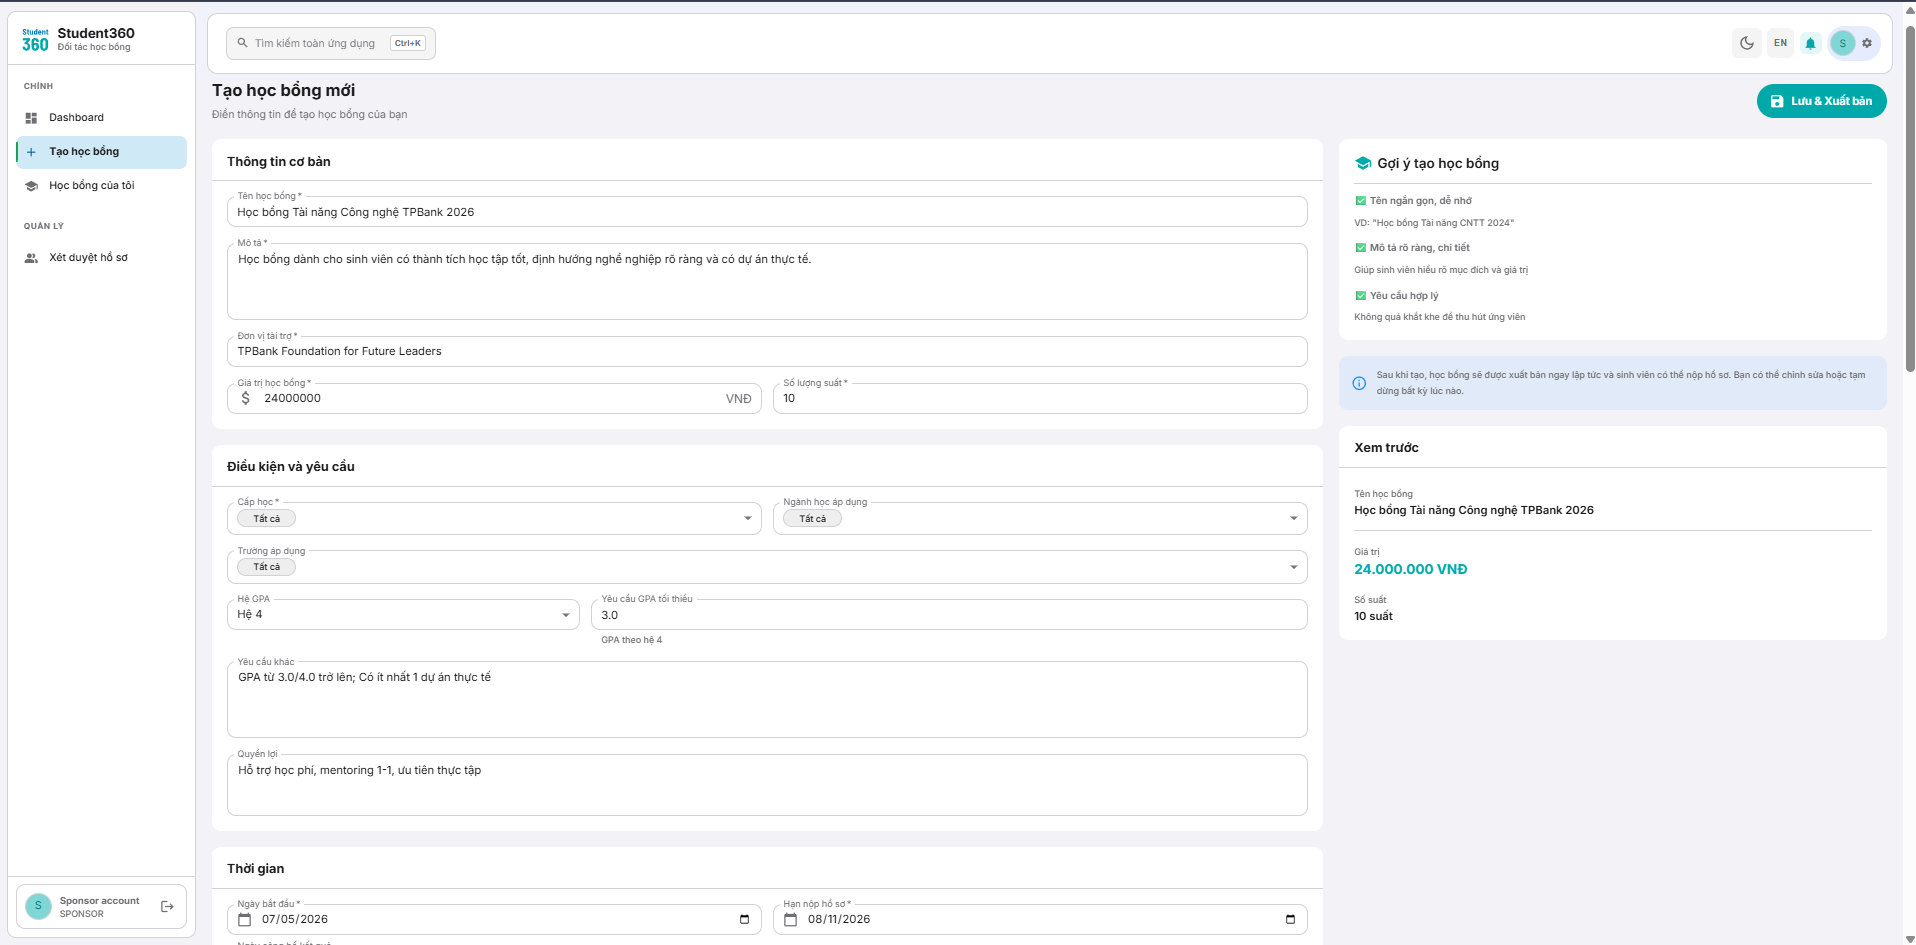
\includegraphics[width=0.85\textwidth]{images/chapter4/webadmin/sponsor-create-scholarship-1.png}%
        }{%
            \rectbox{Màn hình tạo học bổng - phần thông tin chung}
        }

        \vspace{0.4cm}

        \IfFileExists{images/chapter4/webadmin/sponsor-create-scholarship-2.png}{%
            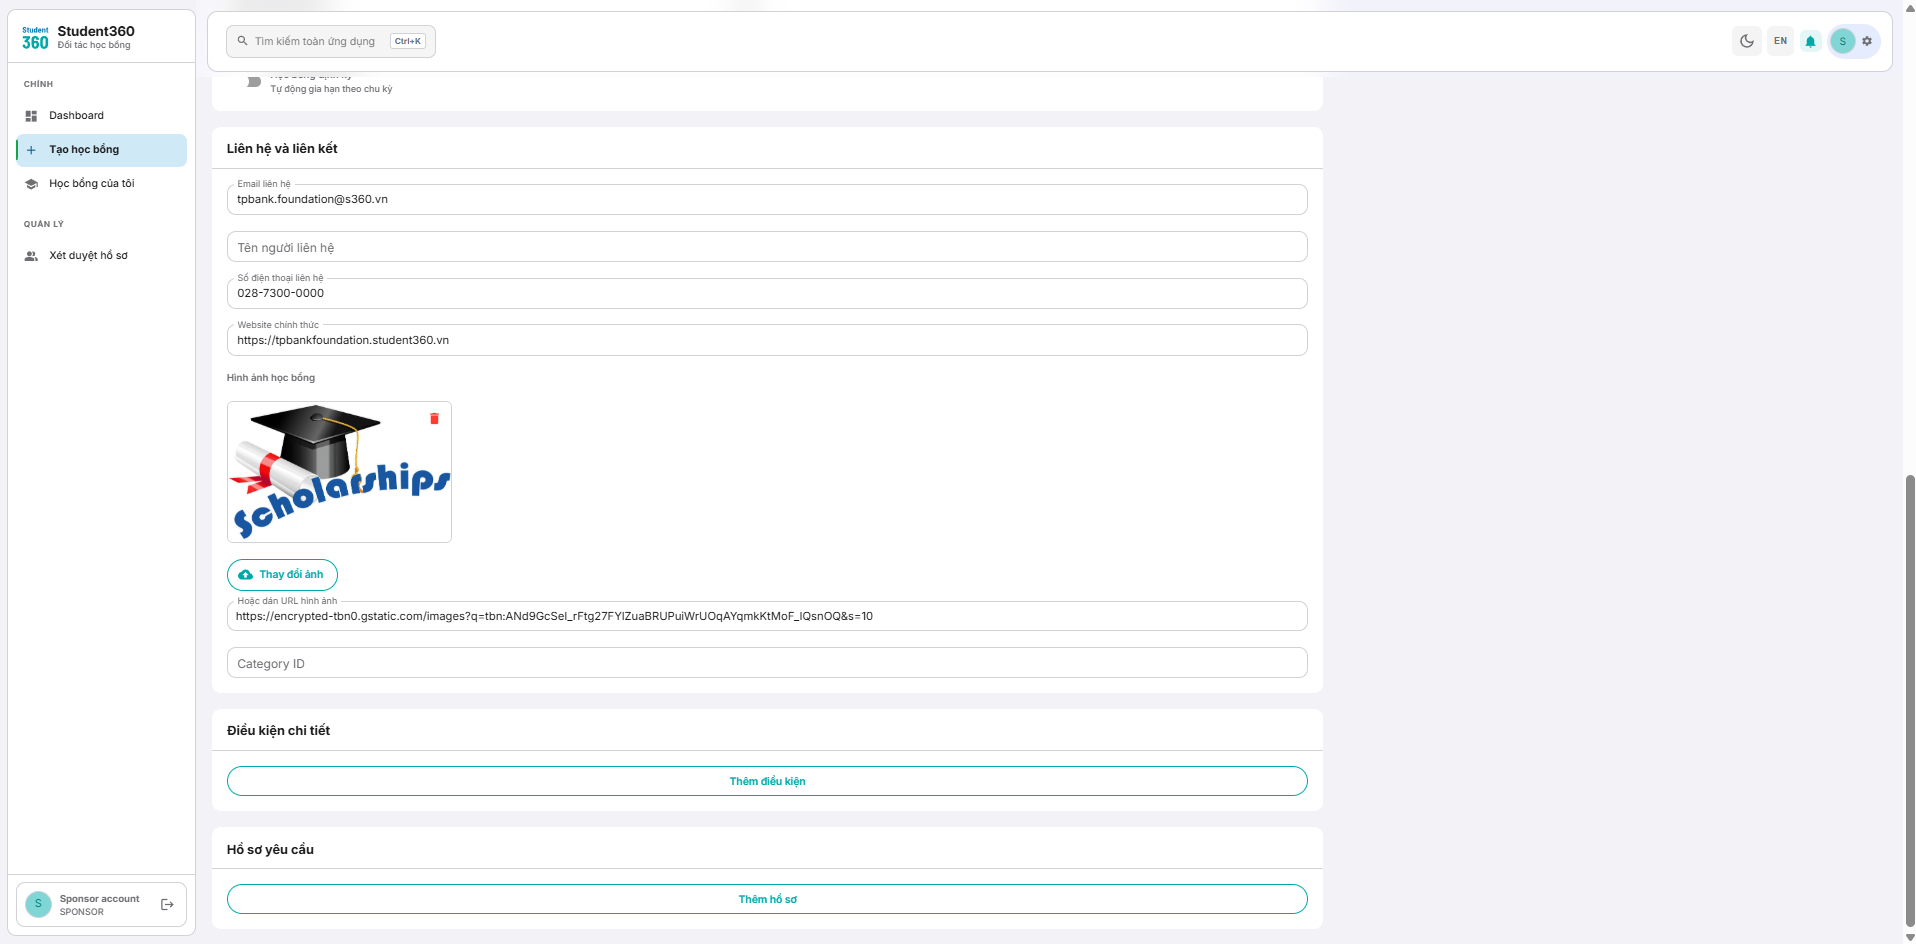
\includegraphics[width=0.85\textwidth]{images/chapter4/webadmin/sponsor-create-scholarship-2.png}%
        }{%
            \rectbox{Màn hình tạo học bổng - phần điều kiện xét tuyển}
        }

        \caption{Giao diện tạo và cấu hình học bổng dành cho nhà tài trợ}
        \label{fig:sponsor-create-scholarship}
    \end{figure}
    \clearpage

    \item \textbf{Xét duyệt hồ sơ học bổng:} Màn hình này cho phép nhà tài trợ xem chi tiết hồ sơ đăng ký của từng sinh viên (GPA, bảng điểm, tài liệu đính kèm) để phê duyệt hoặc từ chối đơn ứng tuyển kèm theo nhận xét phản hồi.
    
    \begin{figure}[H]
        \centering
        \IfFileExists{images/chapter4/webadmin/sponsor-application-review.png}{%
            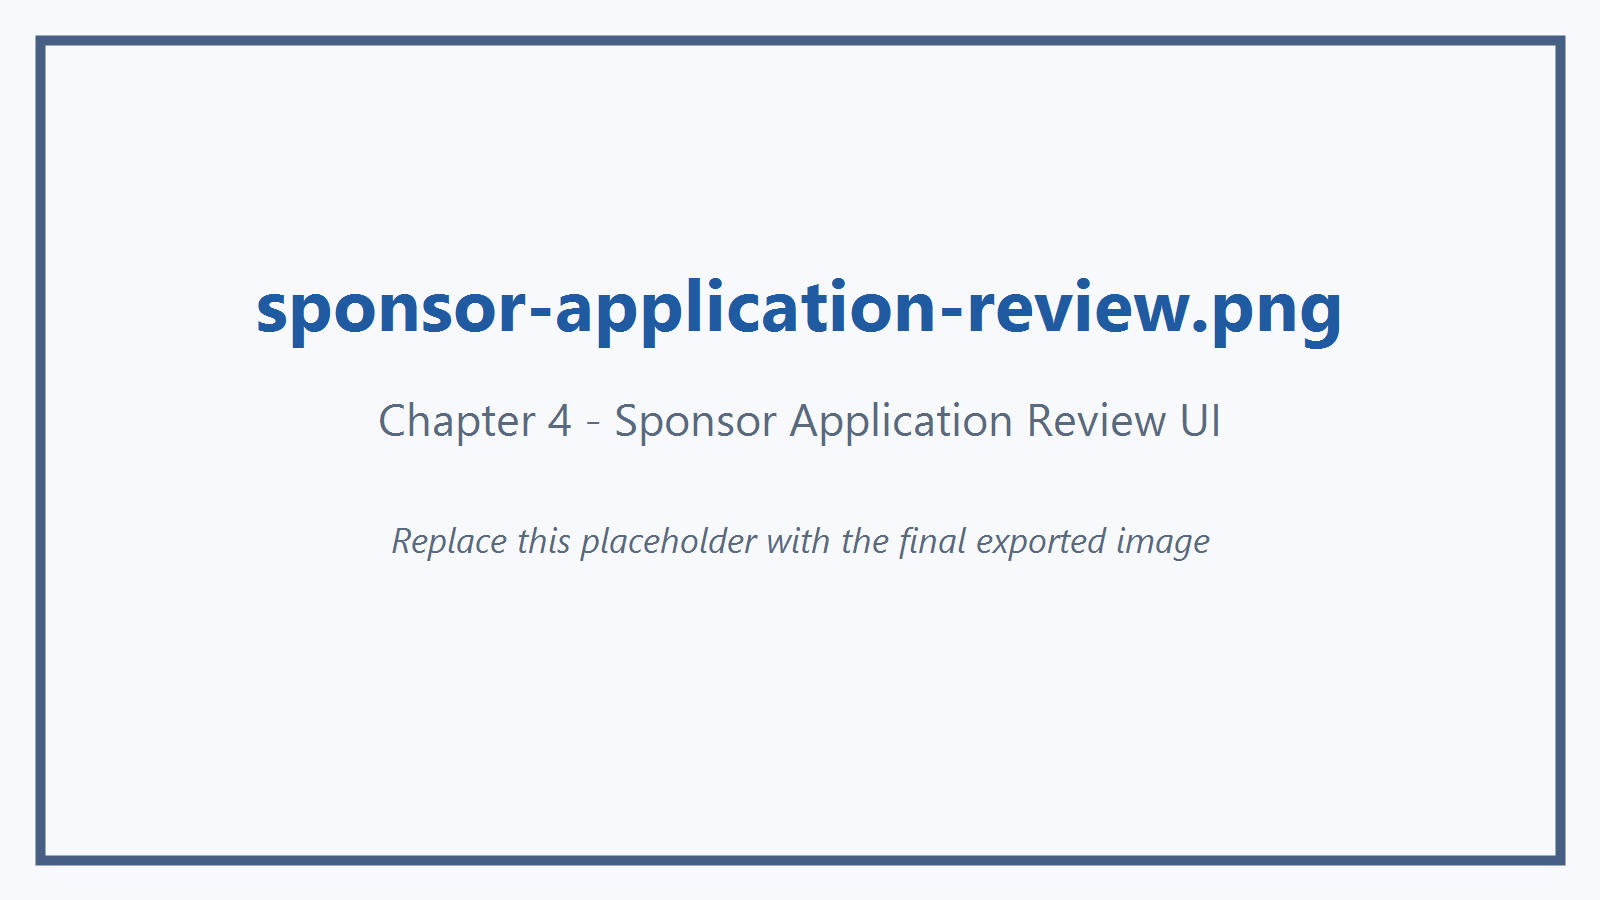
\includegraphics[width=0.85\textwidth]{images/chapter4/webadmin/sponsor-application-review.png}%
        }{%
            \rectbox{Màn hình xét duyệt hồ sơ ứng tuyển học bổng trên Webadmin}
        }
        \caption{Giao diện xét duyệt hồ sơ ứng tuyển học bổng (Duyệt/Từ chối kèm nhận xét)}
        \label{fig:sponsor-application-review}
    \end{figure}
\end{enumerate}


\section{Kiểm thử đơn vị}
\label{sec:kiem-thu-don-vi}
Kiểm thử đơn vị xác minh độc lập từng quy tắc nghiệp vụ của Phân hệ Quản lý Tài chính -- 6 hũ, giao dịch tài chính, cảnh báo tài chính, lịch chuyển tiền tự động, phân loại giao dịch bằng AI, khoản vay và học bổng -- mà không phụ thuộc PostgreSQL, Redis hay AI Service đang chạy: toàn bộ tầng lưu trữ dữ liệu, kết nối cơ sở dữ liệu và mô hình ngôn ngữ đều được giả lập (mock). Phía Backend và AI Service đều dùng bộ công cụ kiểm thử tự động theo đúng ngôn ngữ lập trình tương ứng, với dữ liệu và các dịch vụ ngoài được giả lập hoàn toàn. Không có tài khoản hay hạ tầng ngoài nào được sử dụng ở tầng kiểm thử này.

\subsection{Kết quả kiểm thử đơn vị}
Bảng~\ref{tab:unit-test-summary} tổng hợp kết quả chạy trên cả hai dịch vụ.

\begin{table}[H]
    \centering
    \begin{tabular}{|L{3.6cm}|L{4.2cm}|C{2.2cm}|C{2.2cm}|C{2.8cm}|}
        \hline
        \textbf{Dịch vụ} & \textbf{Phạm vi giả lập} & \textbf{Số bộ kiểm thử} & \textbf{Số test case} & \textbf{Kết quả} \\ \hline
        Backend (NestJS) & Toàn bộ tầng lưu trữ dữ liệu & 48 & 879 & \textbf{879/879 đạt} \\ \hline
        AI Service (FastAPI) & Cơ sở dữ liệu và mô hình ngôn ngữ & 8 & 95 & \textbf{95/95 đạt} \\ \hline
        \textbf{Tổng cộng} & & \textbf{56} & \textbf{974} & \textbf{974/974 đạt (100\%)} \\ \hline
    \end{tabular}
    \caption{Kết quả kiểm thử đơn vị theo dịch vụ}
    \label{tab:unit-test-summary}
\end{table}

Phía Backend, 48 bộ kiểm thử (879 test case) bao phủ toàn bộ các nhóm chức năng của Phân hệ Quản lý Tài chính: quản lý hũ tài chính (kể cả tích hợp AI, phân loại), giao dịch tài chính, cảnh báo tài chính, lịch chuyển tiền tự động, cổng giao tiếp với trợ lý AI, khoản vay, học bổng (từ danh mục, hồ sơ đến quy trình xét duyệt) và quản trị danh mục học thuật.

Phía AI Service, 8 nhóm kiểm thử (95 test case) bao phủ: gắn tag ngân sách cho hành động AI, nhận diện ý định hành động một chạm (one-touch execution), phát hiện bất thường chi tiêu, tổng hợp câu trả lời chat khi công cụ tra cứu trả dữ liệu thô, phân loại giao dịch (ưu tiên bảng tùy chọn cá nhân hóa, ngưỡng độ tin cậy, dự phòng khi mô hình lỗi), phân tích độ phù hợp học bổng, và công thức tính điểm sức khỏe tài chính (tỷ lệ chi tiêu, mức trừ điểm khi có bất thường mức độ nguy hiểm hoặc cảnh báo). Không phát sinh trường hợp nào thất bại ở cả hai dịch vụ.

\subsection{Độ bao phủ mã nguồn (Coverage)}
Độ bao phủ mã nguồn được đo riêng cho các nhóm chức năng thuộc phạm vi Phân hệ Quản lý Tài chính (không tính toàn bộ mã nguồn Backend). Bảng~\ref{tab:unit-test-coverage} trình bày kết quả.

\begin{table}[H]
    \centering
    \begin{tabular}{|L{4.4cm}|C{2.4cm}|C{2.4cm}|C{2.4cm}|C{2.4cm}|}
        \hline
        \textbf{Nhóm chức năng} & \textbf{Statements} & \textbf{Lines} & \textbf{Functions} & \textbf{Branch} \\ \hline
        Quản lý hũ tài chính & 88.99\% & 89.03\% & 96.55\% & 83.87\% \\ \hline
        Lịch chuyển tiền tự động & 93.54\% & 94.79\% & 95.91\% & 84.06\% \\ \hline
        Cảnh báo tài chính & 89.11\% & 92.80\% & 100.0\% & 81.52\% \\ \hline
        Giao dịch tài chính & 93.44\% & 93.88\% & 93.02\% & 90.40\% \\ \hline
        Khoản vay & 85.55\% & 86.90\% & 100.0\% & 100.0\% \\ \hline
        Học bổng & 82.92\% & 82.42\% & 70.38\% & 83.18\% \\ \hline
        Kết nối dịch vụ AI & 81.81\% & 86.20\% & 100.0\% & 100.0\% \\ \hline
        Cổng giao tiếp với trợ lý AI & 80.47\% & 81.25\% & 82.02\% & 70.64\% \\ \hline
        \textbf{Trung bình (8 nhóm chức năng Tài chính)} & \textbf{86.02\%} & \textbf{86.54\%} & \textbf{79.36\%} & \textbf{79.45\%} \\ \hline
    \end{tabular}
    \caption{Độ bao phủ mã nguồn theo nhóm chức năng (phạm vi Phân hệ Quản lý Tài chính)}
    \label{tab:unit-test-coverage}
\end{table}

Hầu hết các nhóm chức năng đều đạt trên 80\% ở cả bốn chỉ số, cho thấy các nhánh xử lý chính đã được kiểm chứng đầy đủ. Cổng giao tiếp với trợ lý AI có Branch coverage thấp hơn phần còn lại (70.64\%) do một phần mã nguồn thuộc các luồng phụ trợ (tư vấn nghề nghiệp, lộ trình học tập) nằm ngoài phạm vi Phân hệ Quản lý Tài chính -- các luồng nghiệp vụ tài chính cốt lõi trong cùng module (thực thi hành động một chạm, gợi ý học bổng qua hội thoại, quản lý phiên chat) đã được kiểm thử đầy đủ hơn.

\section{Kiểm thử tích hợp}
\label{sec:kiem-thu-tich-hop}
Kiểm thử tích hợp xác minh các tầng của hệ thống phối hợp đúng với nhau, ở hai mức độ khác nhau tuỳ đặc thù rủi ro của từng phần:

\begin{itemize}
    \item \textbf{Backend (NestJS):} Dựng tầng tiếp nhận yêu cầu thật (định tuyến, xác thực dữ liệu đầu vào, định dạng lỗi) cùng cơ chế xác thực đăng nhập thật; chỉ tầng xử lý nghiệp vụ (Service) bị giả lập. Cách dựng này đủ để phủ toàn bộ nhánh định tuyến, xác thực dữ liệu đầu vào, phân quyền và mã lỗi trả về mà không cần hạ tầng ngoài.
    \item \textbf{AI Service (FastAPI):} Gọi thẳng ứng dụng thật (không cần khởi động một máy chủ riêng) kết hợp \textbf{PostgreSQL thật}; chỉ mô hình ngôn ngữ (LLM) bị giả lập. Cách dựng này áp dụng cho các chức năng đọc/ghi trực tiếp cơ sở dữ liệu, nơi một câu lệnh truy vấn sai sẽ không thể phát hiện được nếu giả lập cơ sở dữ liệu.
\end{itemize}

\subsection{Kết quả kiểm thử tích hợp}
Bảng~\ref{tab:integration-test-summary} tổng hợp kết quả.

\begin{table}[H]
    \centering
    \begin{tabular}{|L{3.6cm}|L{4.6cm}|C{2.2cm}|C{2.2cm}|C{2.8cm}|}
        \hline
        \textbf{Dịch vụ} & \textbf{Cách dựng} & \textbf{Số bộ kiểm thử} & \textbf{Số test case} & \textbf{Kết quả} \\ \hline
        Backend (NestJS) & Tầng tiếp nhận yêu cầu thật, xử lý nghiệp vụ giả lập & 8 & 139 & \textbf{139/139 đạt} \\ \hline
        AI Service (FastAPI) & Ứng dụng thật, PostgreSQL thật, mô hình ngôn ngữ giả lập & 2 & 16 & \textbf{16/16 đạt} \\ \hline
        \textbf{Tổng cộng} & & \textbf{10} & \textbf{155} & \textbf{155/155 đạt (100\%)} \\ \hline
    \end{tabular}
    \caption{Kết quả kiểm thử tích hợp theo dịch vụ}
    \label{tab:integration-test-summary}
\end{table}

Bảng~\ref{tab:integration-test-backend-detail} liệt kê chi tiết 8 bộ kiểm thử tích hợp phía Backend theo phạm vi nghiệp vụ và trọng tâm kiểm chứng.

\begin{table}[H]
    \centering
    \small
    \begin{tabular}{|L{3.6cm}|L{5.4cm}|C{1.6cm}|L{4.0cm}|}
        \hline
        \textbf{Nhóm chức năng} & \textbf{Phạm vi nghiệp vụ được kiểm thử} & \textbf{Số case} & \textbf{Trọng tâm kiểm chứng} \\ \hline
        Khoản vay & Xem gói vay, xem chi tiết, đăng ký vay, xem khoản vay của tôi, hủy vay & 17 & Kiểm tra hợp lệ số tiền/kỳ hạn vay theo gói, từ chối khi chưa đăng nhập hoặc dữ liệu không hợp lệ \\ \hline
        Cảnh báo tài chính & Kích hoạt các loại cảnh báo (ngưỡng hũ, ngân sách, lịch sắp hết hạn, báo cáo tháng, nhắc giao dịch, bất thường) & 9 & Chuyển tham số đúng xuống cơ chế xử lý cảnh báo, từ chối khi chưa đăng nhập \\ \hline
        Học bổng & Tạo, cập nhật, nộp, xem trạng thái, hủy hồ sơ; đăng ký/hủy đăng ký chương trình & 24 & Vòng đời hồ sơ nháp → nộp → duyệt/hủy \\ \hline
        Quản trị học thuật & Quản lý danh mục trường đại học, môn học, chương trình đào tạo & 19 & Phân quyền (chỉ Quản trị viên), ràng buộc khi dữ liệu còn phụ thuộc \\ \hline
        Quản lý hũ tài chính & Danh sách, chi tiết, tạo, sửa, xoá, tỷ lệ phân bổ, gắn tag & 21 & Kiểm tra hợp lệ dữ liệu đầu vào, chặn sửa hũ hệ thống, chặn trùng tên \\ \hline
        Giao dịch tài chính & Danh sách, tổng hợp, tạo, phân bổ thu nhập, sửa, xoá & 20 & Kiểm tra hợp lệ dữ liệu đầu vào, chặn sửa giao dịch chuyển khoản \\ \hline
        Trợ lý AI & Trò chuyện, phiên chat, thực thi/xác nhận hành động, cảnh báo bất thường, xử lý phản hồi nội bộ từ AI Service & 22 & Xác thực nguồn gọi nội bộ, kiểm tra hợp lệ loại/tham số hành động \\ \hline
        Cảnh báo tài chính (dữ liệu thật) & Cơ chế chống trùng lặp cảnh báo, chạy trực tiếp trên PostgreSQL thật & 7 & Đúng ngữ nghĩa chống trùng lặp trong điều kiện tranh chấp \\ \hline
    \end{tabular}
    \caption{Chi tiết kiểm thử tích hợp Backend theo nhóm chức năng}
    \label{tab:integration-test-backend-detail}
\end{table}

Phía AI Service, 2 nhóm kiểm thử tích hợp (16 test case) chạm PostgreSQL thật: một nhóm 8 case cho chức năng cảnh báo bất thường (đọc/ghi thật bảng cảnh báo, lọc theo trạng thái đã đọc/loại cảnh báo, giới hạn phạm vi theo người dùng, từ chối khi thiếu/sai thông tin xác thực) và một nhóm 8 case cho chức năng phân loại giao dịch (khớp bảng tùy chọn cá nhân hóa thật, dự phòng qua mô hình ngôn ngữ khi không khớp, ngưỡng độ tin cậy, dự phòng về hũ mặc định khi mô hình lỗi).

\section{Quét lỗ hổng bảo mật mã nguồn}
\label{sec:kiem-thu-bao-mat}

Song song với kiểm thử chức năng, mã nguồn Backend được quét lỗ hổng bảo mật bằng công cụ \textbf{Trivy} nhằm đối chiếu các thư viện phụ thuộc của dự án với cơ sở dữ liệu lỗ hổng đã công bố (CVE), từ đó phát hiện sớm các rủi ro bảo mật từ bên thứ ba.

\subsection{Kỹ thuật khắc phục lỗ hổng bảo mật}
Để xử lý các lỗ hổng phát hiện bởi Trivy mà vẫn đảm bảo tính ổn định của ứng dụng, các kỹ thuật sau đã được áp dụng:

\begin{itemize}
    \item \textbf{Nâng cấp gói phụ thuộc trực tiếp:} Đối với các thư viện khai báo trực tiếp trong dự án, tiến hành cập nhật lên phiên bản đã được nhà phát triển vá lỗi bảo mật.
    \item \textbf{Ghi đè phiên bản gói phụ thuộc gián tiếp:} Đối với các lỗ hổng xuất phát từ thư viện con (được kéo vào bởi thư viện khác), áp dụng kỹ thuật ghi đè phiên bản (\textit{dependency overrides}) để buộc hệ thống sử dụng phiên bản an toàn.
    \item \textbf{Xác minh tính ổn định:} Sau khi áp dụng các biện pháp khắc phục, hệ thống được kiểm tra biên dịch lại và đóng gói để đảm bảo không phát sinh xung đột hay lỗi vận hành.
\end{itemize}

\subsection{Kết quả trước và sau khi khắc phục}
Bảng~\ref{tab:trivy-before-after} so sánh kết quả quét lỗ hổng bảo mật trước và sau khi áp dụng các biện pháp xử lý.

\begin{table}[H]
    \centering
    \begin{tabular}{|L{3.2cm}|C{3.2cm}|C{3.2cm}|}
        \hline
        \textbf{Mức độ nghiêm trọng} & \textbf{Trước khắc phục} & \textbf{Sau khắc phục} \\ \hline
        CRITICAL & 3 & \textbf{0} \\ \hline
        HIGH & 30 & \textbf{0} \\ \hline
        MEDIUM & 39 & \textbf{1} \\ \hline
        LOW & 7 & \textbf{1} \\ \hline
        \textbf{Tổng cộng} & \textbf{79} & \textbf{2} \\ \hline
    \end{tabular}
    \caption{Số lỗ hổng bảo mật mã nguồn theo mức độ nghiêm trọng trước và sau khắc phục}
    \label{tab:trivy-before-after}
\end{table}

Kết quả cho thấy toàn bộ các lỗ hổng ở mức nghiêm trọng (CRITICAL) và cao (HIGH) đã được khắc phục triệt để, tổng số lỗ hổng giảm từ 79 xuống còn 2. Hai lỗ hổng còn tồn đọng (1 MEDIUM, 1 LOW) được tạm thời chấp nhận rủi ro do một lỗ hổng đòi hỏi nâng cấp toàn bộ khung làm việc (NestJS) lên phiên bản mới và lỗ hổng còn lại hiện chưa có bản vá từ nhà phát triển.

\section{Đánh giá chất lượng và hiệu năng các chức năng AI}
\label{sec:danh-gia-ai}

\subsection{Phân loại giao dịch tự động}
\label{sec:kiem-thu-api}
Để tối ưu hóa chi phí vận hành và giảm thiểu độ trễ phản hồi, hệ thống áp dụng cơ chế phân loại hỗn hợp gồm hai bước (Hybrid Classification Pipeline):
\begin{itemize}
    \item \textbf{Bước 1 (Khớp từ khóa chính xác):} Hệ thống kiểm tra bảng tùy chọn cá nhân hóa của sinh viên trong cơ sở dữ liệu. Nếu khớp từ khóa (do người dùng từng xác nhận hoặc sửa đổi trước đây), hệ thống trả kết quả đề xuất hũ ngay lập tức mà không cần gọi mô hình AI.
    \item \textbf{Bước 2 (Dự phòng qua LLM):} Khi gặp từ khóa hoặc ngôn ngữ lóng mới, hệ thống gọi mô hình ngôn ngữ lớn để suy luận ngữ nghĩa và đề xuất hũ phù hợp. Khi người dùng xác nhận hoặc chỉnh sửa hũ tài chính thủ công trên giao diện, hệ thống tự động ghi nhận cặp từ khóa -- mã hũ này vào cơ sở dữ liệu, tạo thành một vòng tự học (self-learning loop) cá nhân hóa cho từng sinh viên.
\end{itemize}

\textit{Phương pháp đo:} Độ chính xác được đo trên bộ dữ liệu kiểm thử gồm 300 mô tả giao dịch tiếng Việt tự nhiên (50 mẫu cho mỗi hũ trong 6 hũ tài chính), chạy qua chức năng phân loại thật của hệ thống (Backend kết hợp AI Service), sau đó so khớp kết quả đề xuất với nhãn thực tế đã gán để tính các chỉ số độ chính xác. Bảng~\ref{tab:ai-classify-eval} và Bảng~\ref{tab:ai-classify-prf1} tổng hợp kết quả.

\begin{table}[H]
    \centering
    \begin{tabular}{|L{4.8cm}|C{2.6cm}|C{3.4cm}|C{2.8cm}|}
        \hline
        \textbf{Hũ tài chính} & \textbf{Tổng mẫu thử} & \textbf{Số mẫu phân loại đúng} & \textbf{Độ chính xác (Accuracy)} \\
        \hline
        Chi tiêu thiết yếu (essentials) & 50 & 46 & 92.0\% \\ \hline
        Giáo dục (education) & 50 & 49 & 98.0\% \\ \hline
        Đầu tư (investment) & 50 & 50 & 100.0\% \\ \hline
        Thiện tâm (sharing) & 50 & 50 & 100.0\% \\ \hline
        Hưởng thụ (enjoyment) & 50 & 49 & 98.0\% \\ \hline
        Tiết kiệm (reserve) & 50 & 50 & 100.0\% \\ \hline
        \textbf{Trung bình toàn hệ thống} & \textbf{300} & \textbf{294} & \textbf{98.0\%} \\
        \hline
    \end{tabular}

    \caption{Đánh giá độ chính xác phân loại giao dịch của AI theo hũ tài chính (N=300)}
    \label{tab:ai-classify-eval}
\end{table}

\begin{table}[H]
    \centering
    \begin{tabular}{|L{3.2cm}|C{2.4cm}|C{2.2cm}|C{2.2cm}|}
        \hline
        \textbf{Hũ tài chính} & \textbf{Precision} & \textbf{Recall} & \textbf{F1} \\
        \hline
        Chi tiêu thiết yếu & 100.0\% & 92.0\% & 95.8\% \\ \hline
        Giáo dục & 98.0\% & 98.0\% & 98.0\% \\ \hline
        Đầu tư & 100.0\% & 100.0\% & 100.0\% \\ \hline
        Thiện tâm & 100.0\% & 100.0\% & 100.0\% \\ \hline
        Hưởng thụ & 94.2\% & 98.0\% & 96.1\% \\ \hline
        Tiết kiệm & 96.2\% & 100.0\% & 98.0\% \\ \hline
        \multicolumn{4}{|l|}{Accuracy: \textbf{98.0\%}} \\ \hline
        \multicolumn{4}{|l|}{Macro-F1: \textbf{98.0\%}} \\ \hline
    \end{tabular}

    \caption{Precision / Recall / F1 theo từng hũ tài chính (N=300)}
    \label{tab:ai-classify-prf1}
\end{table}

Mô hình AI đạt độ chính xác \textbf{98.0\%} trên 300 mẫu thử nghiệm và Macro-F1 đạt 98.0\%. Hũ Tiết kiệm (reserve) đạt Accuracy tuyệt đối 100.0\%, không ghi nhận nhầm lẫn nào sang Đầu tư (investment) hay các hũ khác -- ranh giới ngữ nghĩa giữa hành vi cất giữ an toàn (tiết kiệm) và hành vi sinh lời (đầu tư) được phân định rõ. Số lỗi còn lại trong toàn bộ 300 mẫu chỉ chiếm 2.0\% (6/300) và phân bố rải rác, không tập trung vào một cặp hũ cụ thể: 2/50 mẫu Chi tiêu thiết yếu bị nhầm sang Hưởng thụ, 2/50 nhầm sang Tiết kiệm; 1/50 mẫu Giáo dục nhầm sang Hưởng thụ; 1/50 mẫu Hưởng thụ nhầm sang Giáo dục. Ba hũ đạt Accuracy tuyệt đối 100\% (Đầu tư, Thiện tâm, Tiết kiệm) -- trong phạm vi bộ dữ liệu đánh giá, pipeline phân loại đạt kết quả tốt và đồng đều trên cả 6 hũ tài chính, không có hũ nào là điểm yếu có tính hệ thống.

\subsection{Gợi ý học bổng}
\label{sec:danh-gia-hoc-bong}
\textit{Phương pháp đo:} Bộ dữ liệu kiểm thử gồm 150 hồ sơ sinh viên so khớp với 300 học bổng, mỗi hồ sơ được gán sẵn 25 học bổng thực sự phù hợp làm đáp án đúng để đối chiếu. Kết quả dưới đây đo trên chính hàm mà hệ thống dùng để trả danh sách gợi ý hiển thị cho người dùng (gồm bước lọc theo trường/ngành, sau đó sắp xếp theo điểm tổng hợp giữa độ liên quan chủ đề, mức phù hợp GPA và giá trị học bổng), thực thi cục bộ, không qua mạng hay gọi LLM, đảm bảo kết quả tất định và có thể tái lập.

Bảng~\ref{tab:scholarship-matching} tổng hợp kết quả, tính trung bình qua toàn bộ 150 hồ sơ.

\begin{table}[H]
    \centering
    \begin{tabular}{|L{9.0cm}|C{3.0cm}|}
        \hline
        \textbf{Chỉ số} & \textbf{Kết quả} \\ \hline
        Tỷ lệ hồ sơ có học bổng đúng ở vị trí gợi ý đầu tiên & \textbf{92.0\%} \\ \hline
        Tỷ lệ hồ sơ tìm thấy ít nhất 1 học bổng đúng trong 3 gợi ý đầu & \textbf{92.7\%} \\ \hline
        Tỷ lệ hồ sơ tìm thấy ít nhất 1 học bổng đúng trong 5 gợi ý đầu & \textbf{94.7\%} \\ \hline
        Số học bổng đúng trung bình xuất hiện trong 5 gợi ý đầu (trên tổng 25 học bổng đúng/hồ sơ) & \textbf{4.54/5} \\ \hline
        Tỷ lệ học bổng đúng không bị lọc nhầm ở bước lọc trường/ngành & \textbf{100.0\%} \\ \hline
    \end{tabular}
    \caption{Kết quả đánh giá gợi ý học bổng (N=150 hồ sơ, 300 học bổng, 25 học bổng đúng/hồ sơ)}
    \label{tab:scholarship-matching}
\end{table}

Bước lọc theo trường/ngành không loại nhầm bất kỳ học bổng phù hợp nào (100\%). Với 92.0\% hồ sơ, học bổng gợi ý đầu tiên đã là một lựa chọn đúng; 92.7\% hồ sơ tìm thấy ít nhất một học bổng phù hợp ngay trong 3 gợi ý đầu tiên và \textbf{94.7\% hồ sơ} tìm thấy học bổng thực sự phù hợp ngay trong 5 gợi ý đầu tiên -- tức là sinh viên gần như luôn thấy được một học bổng đúng mà không cần cuộn xem nhiều. Trung bình mỗi hồ sơ có 4.54 học bổng đúng xuất hiện trong 5 gợi ý đầu, cho thấy danh sách gợi ý không chỉ đúng ở vị trí đầu mà còn bao phủ tốt phần lớn các lựa chọn phù hợp khác.

\subsection{Trợ lý tư vấn tài chính (Chatbot AI)}
\textit{Phương pháp đo:} Bộ 184 câu hỏi tiếng Việt tự nhiên bao phủ 28 công cụ (tool) của trợ lý AI -- tra cứu số dư/ngân sách/giao dịch hũ, thống kê chi tiêu, lịch chuyển tự động, tư vấn khả năng chi trả và tái phân bổ hũ, gợi ý và tra cứu học bổng, hồ sơ ứng tuyển -- được gửi tuần tự qua tài khoản thật đến hệ thống đang chạy cục bộ (Backend + AI Service). Bảng~\ref{tab:chatbot-eval} tổng hợp kết quả.

\begin{table}[H]
    \centering
    \begin{tabular}{|L{5.0cm}|C{4.4cm}|}
        \hline
        \textbf{Chỉ số} & \textbf{Giá trị} \\ \hline
        Tổng số câu hỏi & 184 \\ \hline
        Trả lời thành công & \textbf{184/184 (100\%)} \\ \hline
        Timeout / lỗi & 0 \\ \hline
        Độ trễ trung bình & 16.3s \\ \hline
        Độ trễ P50 & 14.4s \\ \hline
        Độ trễ P95 & 38.0s \\ \hline
        Độ trễ P99 & 53.9s \\ \hline
        Độ trễ nhỏ nhất / lớn nhất & 0.9s / 65.9s \\ \hline
    \end{tabular}
    \caption{Kết quả kiểm thử trợ lý tư vấn tài chính AI (N=184)}
    \label{tab:chatbot-eval}
\end{table}

Toàn bộ 184 câu hỏi đều được trả lời hợp lệ, không phát sinh timeout hay lỗi thực thi. Với các câu hỏi dạng đếm/tổng số lượng (ví dụ ``có tổng cộng bao nhiêu học bổng trong hệ thống?''), cơ chế trả về của công cụ tra cứu có trường tổng số bản ghi thoả điều kiện độc lập với tham số giới hạn số lượng mà mô hình tự chọn khi gọi công cụ, giúp câu trả lời nhất quán qua nhiều lần hỏi lặp lại cùng nội dung. Đối chiếu độ trễ giữa môi trường cục bộ và môi trường triển khai thực tế (cùng 20 câu hỏi, cùng tài khoản) cho thấy môi trường ảnh hưởng đáng kể đến hình dạng phân bố độ trễ: môi trường triển khai thực tế có trung vị thấp hơn (4.6s so với 14.1s cục bộ) nhưng đuôi phân bố dài hơn rõ rệt (P95 đạt 74.0s so với 23.7s cục bộ), cho thấy phần lớn câu hỏi được xử lý rất nhanh nhưng một số ít câu chịu độ trễ mạng đáng kể.

\subsection{Chi phí vận hành AI}
\textit{Phương pháp đo:} Lượng token đầu vào/đầu ra và chi phí ước tính (theo đơn giá Gemini 2.5 Pro trên Vertex AI) được ghi nhận trực tiếp từ 62 lượt hỏi--đáp thật của trợ lý tư vấn tài chính, đối chiếu khớp với bảng ghi nhận sử dụng AI trong cơ sở dữ liệu hệ thống. Bảng~\ref{tab:ai-token-cost} tổng hợp kết quả.

\begin{table}[H]
    \centering
    \begin{tabular}{|L{5.6cm}|C{3.8cm}|}
        \hline
        \textbf{Chỉ số} & \textbf{Giá trị} \\ \hline
        Tổng số lượt hỏi--đáp & 62 (62/62 thành công) \\ \hline
        Tổng token đầu vào & 816.923 \\ \hline
        Tổng token đầu ra & 11.051 \\ \hline
        Tổng chi phí ước tính & 29.762,19 VND \\ \hline
        Token đầu vào trung bình / lượt & 13.176 \\ \hline
        Token đầu ra trung bình / lượt & 178 \\ \hline
        Chi phí trung bình / lượt & 480,04 VND \\ \hline
    \end{tabular}
    \caption{Chi phí token AI đo trên 62 lượt hỏi--đáp thật}
    \label{tab:ai-token-cost}
\end{table}

Ngoại suy tuyến tính từ mẫu đo được, chi phí vận hành ước tính (chưa gồm các lệnh gọi LLM phụ như phân loại ý định hay kiểm duyệt hành động) tăng theo tần suất sử dụng: khoảng 2.400 VND/người dùng/tháng ở mức 5 tin nhắn/tháng, khoảng 9.601 VND ở mức 20 tin nhắn/tháng, và khoảng 28.802 VND ở mức 60 tin nhắn/tháng -- tương ứng khoảng 2,4 đến 28,8 triệu VND/tháng cho quy mô 1.000 người dùng hoạt động. Công cụ tra cứu danh sách học bổng đầy đủ có chi phí token đầu vào cao gấp khoảng 4,4 lần trung bình chung do trả nguyên dữ liệu danh sách vào ngữ cảnh hội thoại, là công cụ tốn chi phí nhất trong 28 công cụ được đo.

\subsection{Hạn chế của đánh giá AI}
Các kết quả đánh giá AI trình bày ở trên phản ánh đúng phạm vi bộ dữ liệu và điều kiện thử nghiệm hiện tại, nhưng vẫn còn một số giới hạn cần lưu ý. Bộ dữ liệu đánh giá (300 mẫu phân loại giao dịch, 30 hồ sơ so khớp học bổng, 184 câu hỏi tư vấn) tuy đã được mở rộng so với các lần đo trước nhưng vẫn ở quy mô vừa phải so với dữ liệu thực tế phát sinh khi hệ thống có đông người dùng. Việc đánh giá cũng mới dừng ở dữ liệu thử nghiệm được xây dựng có chủ đích, chưa được kiểm chứng trên tập người dùng thật với hành vi và cách diễn đạt đa dạng hơn ở quy mô lớn. Ngoài ra, các chỉ số đo được (accuracy, Top-1, độ trễ) chưa được đối chiếu với một mô hình hay hệ thống tương tự khác để có cơ sở so sánh tương đối. Đây là những hướng cần tiếp tục thực hiện trong các giai đoạn phát triển tiếp theo của đề tài.

\section{Nhận xét và đánh giá tổng quan}

\subsection{Khả năng ứng dụng thực tiễn của hệ thống}
Hệ thống Student360 được thiết kế hướng đến khả năng đưa vào sử dụng thực tế cho đúng các bên liên quan trong hệ sinh thái giáo dục:
\begin{itemize}
    \item \textbf{Sẵn sàng triển khai cho trường đại học và nhà tài trợ:} Phân hệ Webadmin cho phép nhà trường quản lý danh mục đào tạo, môn học và bảng điểm; nhà tài trợ đăng chương trình học bổng và xét duyệt hồ sơ ứng tuyển ngay trên nền tảng, không cần quy trình giấy tờ hay trao đổi thủ công qua nhiều kênh riêng lẻ.
    \item \textbf{Khả năng mở rộng khi số lượng người dùng tăng:} Kiến trúc phân tách rõ ràng giữa ứng dụng di động, trang quản trị, Backend và AI Service theo từng dịch vụ độc lập, cho phép nâng cấp năng lực xử lý của từng thành phần riêng biệt khi lưu lượng sử dụng tăng, thay vì phải mở rộng toàn bộ hệ thống như kiến trúc nguyên khối.
    \item \textbf{Khả năng tích hợp thêm phân hệ mới:} Việc module hóa theo từng nhóm chức năng (tài chính, học thuật, học bổng, trợ lý AI) giúp bổ sung phân hệ mới hoặc mở rộng nghiệp vụ hiện có mà không ảnh hưởng đến các khối chức năng đang vận hành.
    \item \textbf{Có thể sử dụng ngay trong thực tế:} Toàn bộ luồng nghiệp vụ chính -- quản lý 6 hũ tài chính, theo dõi bảng điểm, tìm và ứng tuyển học bổng, trò chuyện với trợ lý AI -- đã được hiện thực hóa đầy đủ trên cả ứng dụng di động và trang quản trị, sẵn sàng để sinh viên, nhà trường và nhà tài trợ trải nghiệm trực tiếp.
\end{itemize}

\subsection{Đóng góp thực tiễn của sản phẩm đối với đối tượng đích}
Student360 không đơn thuần là một công cụ tiện ích riêng lẻ mà hướng tới việc tạo dựng một hệ sinh thái hỗ trợ sinh viên toàn diện:
\begin{itemize}
    \item \textbf{Giải quyết bài toán tài chính cá nhân gắn liền với học tập:} Khác với các app quản lý chi tiêu thông thường, Student360 liên kết số dư của sinh viên với các hũ tài chính đặc thù như học phí, sách vở, đầu tư bản thân. Từ đó, sinh viên có thể chủ động cân bằng giữa chi tiêu sinh hoạt và tích lũy cho việc học tập.
    \item \textbf{Thu hẹp khoảng cách giữa sinh viên và nguồn lực hỗ trợ:} Thông qua cổng học bổng trực tuyến kết hợp thuật toán so khớp thông minh, hệ thống gợi ý các chương trình học bổng phù hợp nhất đến từng hồ sơ sinh viên dựa trên ngành học và GPA. Điều này giúp tăng cơ hội nhận học bổng cho sinh viên nghèo vượt khó hoặc có thành tích xuất sắc, đồng thời giúp nhà tài trợ tìm kiếm đúng ứng viên tiềm năng một cách nhanh chóng.
    \item \textbf{Hỗ trợ ra quyết định thông qua trợ lý AI:} Chatbot tư vấn không chỉ trả lời câu hỏi thông thường mà đóng vai trò là một người cố vấn tài chính ảo, giúp phân tích các thói quen chi tiêu trong quá khứ và đưa ra lời khuyên phân bổ dòng tiền hợp lý, nâng cao kỹ năng quản lý tài chính cho sinh viên ngay từ khi còn ngồi trên ghế nhà trường.
\end{itemize}

\subsection{Đánh giá tổng quan kết quả đạt được}
Qua toàn bộ quá trình triển khai và kiểm thử thực tế, đồ án ứng dụng Student360 đạt được bốn nhóm kết quả nổi bật:
\begin{enumerate}
    \item \textbf{Hoàn thiện chức năng nghiệp vụ:} Tất cả các chức năng theo đặc tả yêu cầu ở Chương 3 đều được hiện thực hóa đầy đủ và, trong phạm vi kiểm thử, hoạt động ổn định trên cả môi trường di động Android/iOS (Student App) lẫn môi trường Web (Admin/Sponsor Portal).
    \item \textbf{Hiệu quả trợ lực từ AI:} Qua đánh giá có thể thấy phân hệ AI đạt kết quả tốt trên bộ dữ liệu đánh giá, với độ chính xác phân loại giao dịch tự động đạt 98.0\% (Macro-F1 đạt 98.0\%) trên 300 mẫu thử nghiệm, gợi ý học bổng đạt Top-1 accuracy 83.3\% và 100\% hồ sơ tìm thấy học bổng đúng trong 3 gợi ý đầu tiên (Mục~\ref{sec:danh-gia-hoc-bong}), và trợ lý tư vấn tài chính trả lời thành công 184/184 câu hỏi (100\%) trong bộ kiểm thử mở rộng.
    \item \textbf{Hiệu năng vận hành thực tế:} Trong phạm vi thử nghiệm, hệ thống hoạt động ổn định qua toàn bộ 155 test case kiểm thử tích hợp (đạt 100\%) trên cả Backend và AI Service. Trợ lý tư vấn tài chính phản hồi thành công toàn bộ 184 câu hỏi với độ trễ trung bình 16.3 giây (P95 đạt 38.0 giây) -- ở mức chấp nhận được với đặc thù truy vấn cần suy luận qua nhiều bước và gọi mô hình ngôn ngữ lớn (Mục~\ref{sec:danh-gia-ai}). Chi phí vận hành AI đo được ở mức thấp, trung bình 480 VND/lượt hỏi--đáp, cho thấy tính khả thi về chi phí khi mở rộng quy mô người dùng.
    \item \textbf{Bảo mật và phân quyền dữ liệu:} Ứng dụng thực thi cơ chế xác thực đăng nhập bắt buộc trên các chức năng nhạy cảm và phân quyền theo vai trò (ví dụ chỉ Quản trị viên được truy cập một số chức năng quản trị danh mục học thuật), được xác minh qua bộ kiểm thử tích hợp ở Mục~\ref{sec:kiem-thu-tich-hop}. Cơ chế cảnh báo tài chính cũng được kiểm chứng giới hạn đúng phạm vi từng người dùng trên cơ sở dữ liệu thật; một trường hợp thao tác chưa giới hạn đúng phạm vi người gọi đã được phát hiện qua kiểm thử tích hợp và ghi nhận theo dõi bằng test case riêng, nhằm xử lý có chủ đích trong các lần cập nhật tiếp theo.
\end{enumerate}

Nhìn chung, hệ thống Student360 đã hoàn thành các mục tiêu đặt ra của đồ án về cả ba trụ cột tài chính, học thuật và học bổng. Kết quả kiểm thử và đánh giá AI trong phạm vi bộ dữ liệu và điều kiện thử nghiệm hiện tại cho thấy hệ thống đáp ứng tốt các yêu cầu chức năng đã đặt ra. Tuy nhiên, như đã nêu ở Mục~\ref{sec:danh-gia-ai}, đánh giá vẫn còn giới hạn về quy mô dữ liệu và chưa được kiểm chứng trên tập người dùng thực tế ở diện rộng. Đây là cơ sở để nhóm tiếp tục mở rộng và hoàn thiện hệ thống trong các giai đoạn phát triển tiếp theo.
